\chapter{Umsetzung}
\label{chap:umsetzung}

% ======================================================================
% Paket A (Entwurf 27.11.2026): Kapiteleinleitung, Containerisierte Bereitstellung, Simulationsumgebung.
% Einfügen in Kapitel/07_Umsetzung.tex direkt nach \chapter{Umsetzung}\label{chap:umsetzung}.
% Code-Bezug: G1 Branch BA-Stable @6a40e47 (Pfade relativ zur Repo-Wurzel), Greifobjekte nach PR #61 @8eb34f4.
% Notizen, Faktenblatt, vorgeschlagene Belege: review/kap7-entwurf/A-notizen.md
% ======================================================================

% ---------------------- Kapiteleinleitung -----------------------------
Die Umgebung setzt die Entscheidungen aus Kapitel~\ref{chap:konzept} entlang des Wegs eines Befehls um, von der Bereitstellung über die Simulation bis zu den Bedienwegen.
Abschnitt~\ref{sec:bereitstellung} zeigt, wo welcher Prozess läuft, und Abschnitt~\ref{sec:simulationsumgebung}, wie MuJoCo die Stelle des Roboters einnimmt.
Die Abschnitte~\ref{sec:fortbewegung_umsetzung} bis~\ref{sec:haende} beschreiben die Funktionsknoten für Beine, Arme und Hände, Abschnitt~\ref{sec:bedienwege} die Anbindung der Bedienwege und Abschnitt~\ref{sec:navigation} ein eingebundenes Modul.
Für alle Abschnitte gilt eine Leseregel: Was nicht ausdrücklich als nur in der Simulation oder nur im Realbetrieb gültig gekennzeichnet ist, gilt in beiden Betriebsarten.
Die Auslegungswerte der Schutzmechanismen aus Tabelle~\ref{tab:schutzmechanismen} stehen bei der jeweiligen Komponente, Messergebnisse folgen erst in Kapitel~\ref{chap:evaluation}.
Welche Quelltextdatei zu welcher Funktionsbezeichnung gehört, ordnet Tabelle~\ref{tab:quelltext} im Anhang zu \pruefen{Anhangtabelle tab:quelltext (TA.1, AP 5) anlegen}.
% DB: Gliederung nach review/kap7-entwurf/plan-kap7.md §1.1 und §2; keine Sachaussage über Code.

% ======================================================================
\section{Containerisierte Bereitstellung}
\label{sec:bereitstellung}
% ======================================================================
Die Umgebung ist auf drei Container-Abbilder verteilt, getrennt danach, welche Software nur in einer Betriebsart gebraucht wird.
Damit setzt sie die Container-Profile aus Abschnitt~\ref{sec:container_profile} um, mit denen sie nach A6 und A7 ohne native Installation auf neuen PCs läuft (Abschnitt~\ref{sec:container}).
Das Abbild der Physiksimulation enthält MuJoCo, das Python-SDK des Herstellers und die Kopplungsschicht, aber kein ROS~2.
Die beiden Abbilder der Steuerung bauen auf ROS~2 Humble auf und enthalten dieselben Funktionsknoten.
Nur das Abbild für die Simulation bringt zusätzlich die Laufzeitumgebung für die Lauf-Policies im Format ONNX mit, weil am realen Roboter der Onboard-Regler läuft (Abschnitt~\ref{sec:fortbewegungspfade}).
Tabelle~\ref{tab:container} fasst die drei Abbilder zusammen.
% DB: g1pilot/docker/Dockerfile.mujoco:1-30, g1pilot/docker/Dockerfile.sim:1-85, g1pilot/docker/Dockerfile.real:1-84 @6a40e47

\begin{table}[htbp]
    \tabstil
    \centering
    \caption[Container-Abbilder der Umgebung]{Container-Abbilder der Umgebung. Eine Compose-Datei startet sie in zwei Profilen, alle Container teilen das Netzwerk des Host-PCs.}
    \label{tab:container}
    \begin{tabularx}{\textwidth}{|>{\raggedright\arraybackslash}p{2.9cm}|>{\raggedright\arraybackslash}p{2.6cm}|L|>{\raggedright\arraybackslash}p{1.5cm}|}\hline
        \tabkopfzeile \tabkopf{Abbild} & \tabkopf{Basis} & \tabkopf{Inhalt} & \tabkopf{Profil}\\\hline
        Physik\-simulation & Ubuntu 22.04 & MuJoCo, Python-SDK des Herstellers, Kopplungsschicht, Szenen und Robotermodelle, kein ROS~2 & sim\\\hline
        Steuerung Simulation & ROS~2 Humble & Funktionsknoten, Bedienoberfläche, 3D-Anzeige, Laufzeit für ONNX-Netze der Lauf-Policies & sim\\\hline
        Steuerung Realbetrieb & ROS~2 Humble & Funktionsknoten, Bedienoberfläche, 3D-Anzeige, Zugriff auf Eingabegeräte, keine Laufzeit für Lauf-Policies \pruefen{im Real-Abbild fehlt auch die Planungsbibliothek OMPL, der Bahnplaner nutzt dort seinen eingebauten Rückfallweg: gewollt?} & real\\\hline
    \end{tabularx}
\end{table}
% DB: g1pilot/docker/Dockerfile.mujoco:1,14-24; g1pilot/docker/Dockerfile.sim:1,9-31,43-56; g1pilot/docker/Dockerfile.real:1-7,15-50 (kein ompl, kein onnxruntime);
%     g1pilot/docker-compose.yml:25-31 (mujoco-sim, profiles sim), :67-75 (g1pilot-sim), :159-169 (g1pilot-real, privileged für /dev/input) @6a40e47

Tabelle~\ref{tab:container} zeigt, dass sich die beiden Steuerungsabbilder nur in Ergänzungen unterscheiden, nicht in den Funktionsknoten.
Die Wahl der Betriebsart trifft allein das gestartete Profil: Im Profil \emph{sim} laufen Physiksimulation und Steuerung als zwei Container, im Profil \emph{real} nur die Steuerung.
Das Profil setzt eine Umgebungsvariable, die die Funktionsknoten an einer einzigen Stelle auswerten (Abschnitt~\ref{sec:sim_real_schalter}).
Alle Container teilen das Netzwerk des Host-PCs, sodass die Steuerung die Simulation über dessen Loopback-Schnittstelle und den Roboter über dessen Netzwerkkarte erreicht.
Der Verkehr von ROS~2 ist per Konfiguration auf die Loopback-Schnittstelle beschränkt und gelangt so nicht in das Netz des Roboters.
Abbildung~\ref{fig:verteilung} zeigt die Verteilung der Prozesse in beiden Profilen.
% DB: g1pilot/docker-compose.yml:10-17 (network_mode host), :32, :84 (G1_SIM_MODE=true), :172 (false); g1pilot/g1pilot/utils/common.py:24-55;
%     g1pilot/docker/cyclonedds.xml:1-16 (nur lo, kein Multicast), g1pilot/docker/Dockerfile.real:74-81 @6a40e47

\begin{figure}[htbp]
  \centering
  % Verteilung der Prozesse auf Host und Container, a) Simulation, b) Realbetrieb (Kap. Umsetzung, fig:verteilung).
% Eigene Darstellung, keine Quelle in der Caption.
% Basis: G1@6a40e47 g1pilot/docker-compose.yml:10-17 (network_mode host, Code eingebunden), :25-66 (Container Physiksimulation),
%   :67-153 (Steuerung Simulation, ROS_DOMAIN_ID=0, Bluetooth über System-D-Bus), :159-261 (Steuerung Realbetrieb,
%   ROS_DOMAIN_ID=1, ROBOT_INTERFACE, Hände per Modbus TCP 192.168.123.210/.211);
%   g1pilot/utils/common.py:6-23 (Unitree-DDS Domain 1/lo bzw. 0/Netzwerkkarte);
%   unitree_mujoco/simulate_python/scene_state_publisher.py:1-22 (UDP von der Simulation zum ROS-Container);
%   g1pilot/g1_gui.py:1-23 und start.sh:51-58 (Startmenü auf dem Host); docker/sim_shutdown_watcher.sh, real_shutdown_watcher.sh (Wächter auf dem Host);
%   g1pilot/start_gui/netsetup.py:1-13 (Einrichtung der Netzwerkkarte für das Roboter-LAN);
%   Arm-API per HTTP: Kap. 6 tab:andockpunkte („beide, lokal“).
% Stil: ba-grafik.tex. Einbinden: % Verteilung der Prozesse auf Host und Container, a) Simulation, b) Realbetrieb (Kap. Umsetzung, fig:verteilung).
% Eigene Darstellung, keine Quelle in der Caption.
% Basis: G1@6a40e47 g1pilot/docker-compose.yml:10-17 (network_mode host, Code eingebunden), :25-66 (Container Physiksimulation),
%   :67-153 (Steuerung Simulation, ROS_DOMAIN_ID=0, Bluetooth über System-D-Bus), :159-261 (Steuerung Realbetrieb,
%   ROS_DOMAIN_ID=1, ROBOT_INTERFACE, Hände per Modbus TCP 192.168.123.210/.211);
%   g1pilot/utils/common.py:6-23 (Unitree-DDS Domain 1/lo bzw. 0/Netzwerkkarte);
%   unitree_mujoco/simulate_python/scene_state_publisher.py:1-22 (UDP von der Simulation zum ROS-Container);
%   g1pilot/g1_gui.py:1-23 und start.sh:51-58 (Startmenü auf dem Host); docker/sim_shutdown_watcher.sh, real_shutdown_watcher.sh (Wächter auf dem Host);
%   g1pilot/start_gui/netsetup.py:1-13 (Einrichtung der Netzwerkkarte für das Roboter-LAN);
%   Arm-API per HTTP: Kap. 6 tab:andockpunkte („beide, lokal“).
% Stil: ba-grafik.tex. Einbinden: % Verteilung der Prozesse auf Host und Container, a) Simulation, b) Realbetrieb (Kap. Umsetzung, fig:verteilung).
% Eigene Darstellung, keine Quelle in der Caption.
% Basis: G1@6a40e47 g1pilot/docker-compose.yml:10-17 (network_mode host, Code eingebunden), :25-66 (Container Physiksimulation),
%   :67-153 (Steuerung Simulation, ROS_DOMAIN_ID=0, Bluetooth über System-D-Bus), :159-261 (Steuerung Realbetrieb,
%   ROS_DOMAIN_ID=1, ROBOT_INTERFACE, Hände per Modbus TCP 192.168.123.210/.211);
%   g1pilot/utils/common.py:6-23 (Unitree-DDS Domain 1/lo bzw. 0/Netzwerkkarte);
%   unitree_mujoco/simulate_python/scene_state_publisher.py:1-22 (UDP von der Simulation zum ROS-Container);
%   g1pilot/g1_gui.py:1-23 und start.sh:51-58 (Startmenü auf dem Host); docker/sim_shutdown_watcher.sh, real_shutdown_watcher.sh (Wächter auf dem Host);
%   g1pilot/start_gui/netsetup.py:1-13 (Einrichtung der Netzwerkkarte für das Roboter-LAN);
%   Arm-API per HTTP: Kap. 6 tab:andockpunkte („beide, lokal“).
% Stil: ba-grafik.tex. Einbinden: \input{Bilder/tikz/verteilung-container} in einer figure-Umgebung. Nicht skalieren.
\begin{tikzpicture}[ba]
  \tikzset{
    klein/.style={font=\footnotesize, text=baGrau},
    host/.style={draw=baGrau, ba duenn, fill=baHellgrau!25, rounded corners=3pt},
    behaelter/.style={draw=baGrau, ba duenn, fill=white, rounded corners=3pt},
    proz/.style={ba block, font=\footnotesize, minimum width=26mm, minimum height=10mm, text width=24mm},
    oben/.style={ba block, font=\footnotesize, minimum width=22mm, minimum height=9mm, text width=20mm},
    aussen/.style={ba block, font=\footnotesize, minimum width=21mm, minimum height=9mm, text width=19mm},
    kDDS/.style={draw=baGruen, ba dick},
    kROS/.style={draw=baBlau, ba normal},
    kUDP/.style={draw=baGrau, ba normal, dash pattern=on 2pt off 2pt},
    kHTTP/.style={draw=baGrau, ba normal, dash pattern=on 0.8pt off 1.6pt},
    kBT/.style={draw=baHellblau, ba normal, dash pattern=on 4pt off 1.5pt on 0.8pt off 1.5pt},
    kMB/.style={draw=baBlau, ba normal, dash pattern=on 7pt off 2pt},
    kStart/.style={draw=baGrau, ba duenn, ->},
  }
  % Raster je Teilbild (x0 = 0 bzw. 8,3): Host 0..7,7 x 1,3..7,5; Container links 0,25..3,35, rechts 4,35..7,45, je 1,6..5,8;
  % obere Reihe y = 6,7; Prozessreihe A y = 4,15, Reihe B y = 2,55; Geräte außerhalb y = 0,45.
  \foreach \x/\k/\titel in {0/a/a) Simulation, 8.3/b/b) Realbetrieb} {
    \draw[host] (\x,1.3) rectangle (\x+7.7,7.8);
    \node[klein, anchor=north west, inner sep=0pt] at (\x+0.2,7.68) {Host-PC};
    \node[oben] at (\x+1.35,6.65) {Startmenü};
    \node[oben] at (\x+3.85,6.65) {Wächter};
    \node[oben] (FP\k) at (\x+6.35,6.65) {Fremdes\\Programm};
    \draw[behaelter] (\x+4.35,1.6) rectangle (\x+7.45,5.8);
    \node[ba teiltitel] at (\x+3.85,-0.35) {\titel};
  }
  % ---------------- a) Simulation ----------------
  \draw[behaelter] (0.25,1.6) rectangle (3.35,5.8);
  \node[klein, anchor=north west, align=left, inner sep=0pt] at (0.4,5.65) {Container\\Physiksimulation};
  \node[klein, anchor=north west, align=left, inner sep=0pt] at (4.5,5.65) {Container\\Steuerung};
  \node[proz, minimum height=26mm] (SIM) at (1.8,3.35) {MuJoCo-\\Simulation mit\\Kopplungs-\\schicht};
  \node[proz] (FKa) at (5.9,4.15) {Funktions-\\knoten};
  \node[proz] (BOa) at (5.9,2.55) {Bedien-\\oberfläche};
  \node[aussen] (SPa) at (5.9,0.45) {Smartphone};
  \draw[kDDS] (SIM.east |- 0,4.35) -- (FKa.west |- 0,4.35);
  \draw[kUDP] (SIM.east |- 0,3.95) -- (FKa.west |- 0,3.95);
  \draw[kROS] (FKa) -- (BOa);
  \draw[kHTTP] (7.0,0 |- FPa.south) -- (7.0,0 |- FKa.north);
  \draw[kBT] (SPa.north) -- (BOa.south);
  % ---------------- b) Realbetrieb ----------------
  \node[klein, anchor=north west, align=left, inner sep=0pt] at (12.8,5.65) {Container\\Steuerung};
  \node[proz] (NIC) at (10.1,4.15) {Netzwerkkarte\\(Roboter-LAN)};
  \node[proz] (FKb) at (14.2,4.15) {Funktions-\\knoten};
  \node[proz] (BOb) at (14.2,2.55) {Bedien-\\oberfläche};
  \node[aussen] (G1) at (9.25,0.45) {Unitree G1};
  \node[aussen] (HA) at (11.6,0.45) {Inspire-\\Hände};
  \node[aussen] (SPb) at (14.2,0.45) {Smartphone};
  \draw[kDDS] (NIC.east |- 0,4.35) -- (FKb.west |- 0,4.35);
  \draw[kMB] (NIC.east |- 0,3.95) -- (FKb.west |- 0,3.95);
  \draw[kDDS] (9.25,0 |- NIC.south) -- (G1.north);
  \draw[kMB] (10.85,0 |- NIC.south) -- (10.85,0 |- HA.north);
  \draw[kROS] (FKb) -- (BOb);
  \draw[kHTTP] (15.3,0 |- FPb.south) -- (15.3,0 |- FKb.north);
  \draw[kBT] (SPb.north) -- (BOb.south);
  \draw[kStart] (9.65,6.2) -- node[klein, right, pos=0.45] {richtet ein} (9.65,0 |- NIC.north);
  % Trenner zwischen den Teilbildern
  \draw[ba trenner] (8.15,-0.6) -- (8.15,7.8);
  % ---------------- Legende (eine Zeile) ----------------
  \foreach \lx/\stil/\text in {0.4/kDDS/DDS, 2.7/kROS/ROS~2, 5.1/kUDP/UDP,
                               7.3/kHTTP/HTTP, 9.6/kBT/Bluetooth, 12.6/kMB/Modbus TCP} {
    \draw[\stil] (\lx,-1.2) -- (\lx+0.8,-1.2);
    \node[font=\footnotesize, anchor=west, inner sep=2pt] at (\lx+0.85,-1.2) {\text};
  }
\end{tikzpicture}
 in einer figure-Umgebung. Nicht skalieren.
\begin{tikzpicture}[ba]
  \tikzset{
    klein/.style={font=\footnotesize, text=baGrau},
    host/.style={draw=baGrau, ba duenn, fill=baHellgrau!25, rounded corners=3pt},
    behaelter/.style={draw=baGrau, ba duenn, fill=white, rounded corners=3pt},
    proz/.style={ba block, font=\footnotesize, minimum width=26mm, minimum height=10mm, text width=24mm},
    oben/.style={ba block, font=\footnotesize, minimum width=22mm, minimum height=9mm, text width=20mm},
    aussen/.style={ba block, font=\footnotesize, minimum width=21mm, minimum height=9mm, text width=19mm},
    kDDS/.style={draw=baGruen, ba dick},
    kROS/.style={draw=baBlau, ba normal},
    kUDP/.style={draw=baGrau, ba normal, dash pattern=on 2pt off 2pt},
    kHTTP/.style={draw=baGrau, ba normal, dash pattern=on 0.8pt off 1.6pt},
    kBT/.style={draw=baHellblau, ba normal, dash pattern=on 4pt off 1.5pt on 0.8pt off 1.5pt},
    kMB/.style={draw=baBlau, ba normal, dash pattern=on 7pt off 2pt},
    kStart/.style={draw=baGrau, ba duenn, ->},
  }
  % Raster je Teilbild (x0 = 0 bzw. 8,3): Host 0..7,7 x 1,3..7,5; Container links 0,25..3,35, rechts 4,35..7,45, je 1,6..5,8;
  % obere Reihe y = 6,7; Prozessreihe A y = 4,15, Reihe B y = 2,55; Geräte außerhalb y = 0,45.
  \foreach \x/\k/\titel in {0/a/a) Simulation, 8.3/b/b) Realbetrieb} {
    \draw[host] (\x,1.3) rectangle (\x+7.7,7.8);
    \node[klein, anchor=north west, inner sep=0pt] at (\x+0.2,7.68) {Host-PC};
    \node[oben] at (\x+1.35,6.65) {Startmenü};
    \node[oben] at (\x+3.85,6.65) {Wächter};
    \node[oben] (FP\k) at (\x+6.35,6.65) {Fremdes\\Programm};
    \draw[behaelter] (\x+4.35,1.6) rectangle (\x+7.45,5.8);
    \node[ba teiltitel] at (\x+3.85,-0.35) {\titel};
  }
  % ---------------- a) Simulation ----------------
  \draw[behaelter] (0.25,1.6) rectangle (3.35,5.8);
  \node[klein, anchor=north west, align=left, inner sep=0pt] at (0.4,5.65) {Container\\Physiksimulation};
  \node[klein, anchor=north west, align=left, inner sep=0pt] at (4.5,5.65) {Container\\Steuerung};
  \node[proz, minimum height=26mm] (SIM) at (1.8,3.35) {MuJoCo-\\Simulation mit\\Kopplungs-\\schicht};
  \node[proz] (FKa) at (5.9,4.15) {Funktions-\\knoten};
  \node[proz] (BOa) at (5.9,2.55) {Bedien-\\oberfläche};
  \node[aussen] (SPa) at (5.9,0.45) {Smartphone};
  \draw[kDDS] (SIM.east |- 0,4.35) -- (FKa.west |- 0,4.35);
  \draw[kUDP] (SIM.east |- 0,3.95) -- (FKa.west |- 0,3.95);
  \draw[kROS] (FKa) -- (BOa);
  \draw[kHTTP] (7.0,0 |- FPa.south) -- (7.0,0 |- FKa.north);
  \draw[kBT] (SPa.north) -- (BOa.south);
  % ---------------- b) Realbetrieb ----------------
  \node[klein, anchor=north west, align=left, inner sep=0pt] at (12.8,5.65) {Container\\Steuerung};
  \node[proz] (NIC) at (10.1,4.15) {Netzwerkkarte\\(Roboter-LAN)};
  \node[proz] (FKb) at (14.2,4.15) {Funktions-\\knoten};
  \node[proz] (BOb) at (14.2,2.55) {Bedien-\\oberfläche};
  \node[aussen] (G1) at (9.25,0.45) {Unitree G1};
  \node[aussen] (HA) at (11.6,0.45) {Inspire-\\Hände};
  \node[aussen] (SPb) at (14.2,0.45) {Smartphone};
  \draw[kDDS] (NIC.east |- 0,4.35) -- (FKb.west |- 0,4.35);
  \draw[kMB] (NIC.east |- 0,3.95) -- (FKb.west |- 0,3.95);
  \draw[kDDS] (9.25,0 |- NIC.south) -- (G1.north);
  \draw[kMB] (10.85,0 |- NIC.south) -- (10.85,0 |- HA.north);
  \draw[kROS] (FKb) -- (BOb);
  \draw[kHTTP] (15.3,0 |- FPb.south) -- (15.3,0 |- FKb.north);
  \draw[kBT] (SPb.north) -- (BOb.south);
  \draw[kStart] (9.65,6.2) -- node[klein, right, pos=0.45] {richtet ein} (9.65,0 |- NIC.north);
  % Trenner zwischen den Teilbildern
  \draw[ba trenner] (8.15,-0.6) -- (8.15,7.8);
  % ---------------- Legende (eine Zeile) ----------------
  \foreach \lx/\stil/\text in {0.4/kDDS/DDS, 2.7/kROS/ROS~2, 5.1/kUDP/UDP,
                               7.3/kHTTP/HTTP, 9.6/kBT/Bluetooth, 12.6/kMB/Modbus TCP} {
    \draw[\stil] (\lx,-1.2) -- (\lx+0.8,-1.2);
    \node[font=\footnotesize, anchor=west, inner sep=2pt] at (\lx+0.85,-1.2) {\text};
  }
\end{tikzpicture}
 in einer figure-Umgebung. Nicht skalieren.
\begin{tikzpicture}[ba]
  \tikzset{
    klein/.style={font=\footnotesize, text=baGrau},
    host/.style={draw=baGrau, ba duenn, fill=baHellgrau!25, rounded corners=3pt},
    behaelter/.style={draw=baGrau, ba duenn, fill=white, rounded corners=3pt},
    proz/.style={ba block, font=\footnotesize, minimum width=26mm, minimum height=10mm, text width=24mm},
    oben/.style={ba block, font=\footnotesize, minimum width=22mm, minimum height=9mm, text width=20mm},
    aussen/.style={ba block, font=\footnotesize, minimum width=21mm, minimum height=9mm, text width=19mm},
    kDDS/.style={draw=baGruen, ba dick},
    kROS/.style={draw=baBlau, ba normal},
    kUDP/.style={draw=baGrau, ba normal, dash pattern=on 2pt off 2pt},
    kHTTP/.style={draw=baGrau, ba normal, dash pattern=on 0.8pt off 1.6pt},
    kBT/.style={draw=baHellblau, ba normal, dash pattern=on 4pt off 1.5pt on 0.8pt off 1.5pt},
    kMB/.style={draw=baBlau, ba normal, dash pattern=on 7pt off 2pt},
    kStart/.style={draw=baGrau, ba duenn, ->},
  }
  % Raster je Teilbild (x0 = 0 bzw. 8,3): Host 0..7,7 x 1,3..7,5; Container links 0,25..3,35, rechts 4,35..7,45, je 1,6..5,8;
  % obere Reihe y = 6,7; Prozessreihe A y = 4,15, Reihe B y = 2,55; Geräte außerhalb y = 0,45.
  \foreach \x/\k/\titel in {0/a/a) Simulation, 8.3/b/b) Realbetrieb} {
    \draw[host] (\x,1.3) rectangle (\x+7.7,7.8);
    \node[klein, anchor=north west, inner sep=0pt] at (\x+0.2,7.68) {Host-PC};
    \node[oben] at (\x+1.35,6.65) {Startmenü};
    \node[oben] at (\x+3.85,6.65) {Wächter};
    \node[oben] (FP\k) at (\x+6.35,6.65) {Fremdes\\Programm};
    \draw[behaelter] (\x+4.35,1.6) rectangle (\x+7.45,5.8);
    \node[ba teiltitel] at (\x+3.85,-0.35) {\titel};
  }
  % ---------------- a) Simulation ----------------
  \draw[behaelter] (0.25,1.6) rectangle (3.35,5.8);
  \node[klein, anchor=north west, align=left, inner sep=0pt] at (0.4,5.65) {Container\\Physiksimulation};
  \node[klein, anchor=north west, align=left, inner sep=0pt] at (4.5,5.65) {Container\\Steuerung};
  \node[proz, minimum height=26mm] (SIM) at (1.8,3.35) {MuJoCo-\\Simulation mit\\Kopplungs-\\schicht};
  \node[proz] (FKa) at (5.9,4.15) {Funktions-\\knoten};
  \node[proz] (BOa) at (5.9,2.55) {Bedien-\\oberfläche};
  \node[aussen] (SPa) at (5.9,0.45) {Smartphone};
  \draw[kDDS] (SIM.east |- 0,4.35) -- (FKa.west |- 0,4.35);
  \draw[kUDP] (SIM.east |- 0,3.95) -- (FKa.west |- 0,3.95);
  \draw[kROS] (FKa) -- (BOa);
  \draw[kHTTP] (7.0,0 |- FPa.south) -- (7.0,0 |- FKa.north);
  \draw[kBT] (SPa.north) -- (BOa.south);
  % ---------------- b) Realbetrieb ----------------
  \node[klein, anchor=north west, align=left, inner sep=0pt] at (12.8,5.65) {Container\\Steuerung};
  \node[proz] (NIC) at (10.1,4.15) {Netzwerkkarte\\(Roboter-LAN)};
  \node[proz] (FKb) at (14.2,4.15) {Funktions-\\knoten};
  \node[proz] (BOb) at (14.2,2.55) {Bedien-\\oberfläche};
  \node[aussen] (G1) at (9.25,0.45) {Unitree G1};
  \node[aussen] (HA) at (11.6,0.45) {Inspire-\\Hände};
  \node[aussen] (SPb) at (14.2,0.45) {Smartphone};
  \draw[kDDS] (NIC.east |- 0,4.35) -- (FKb.west |- 0,4.35);
  \draw[kMB] (NIC.east |- 0,3.95) -- (FKb.west |- 0,3.95);
  \draw[kDDS] (9.25,0 |- NIC.south) -- (G1.north);
  \draw[kMB] (10.85,0 |- NIC.south) -- (10.85,0 |- HA.north);
  \draw[kROS] (FKb) -- (BOb);
  \draw[kHTTP] (15.3,0 |- FPb.south) -- (15.3,0 |- FKb.north);
  \draw[kBT] (SPb.north) -- (BOb.south);
  \draw[kStart] (9.65,6.2) -- node[klein, right, pos=0.45] {richtet ein} (9.65,0 |- NIC.north);
  % Trenner zwischen den Teilbildern
  \draw[ba trenner] (8.15,-0.6) -- (8.15,7.8);
  % ---------------- Legende (eine Zeile) ----------------
  \foreach \lx/\stil/\text in {0.4/kDDS/DDS, 2.7/kROS/ROS~2, 5.1/kUDP/UDP,
                               7.3/kHTTP/HTTP, 9.6/kBT/Bluetooth, 12.6/kMB/Modbus TCP} {
    \draw[\stil] (\lx,-1.2) -- (\lx+0.8,-1.2);
    \node[font=\footnotesize, anchor=west, inner sep=2pt] at (\lx+0.85,-1.2) {\text};
  }
\end{tikzpicture}

  \caption[Verteilung der Prozesse auf Host und Container]{Verteilung der Prozesse auf Host-PC und Container in a) der Simulation und b) dem Realbetrieb. Die Herstellerschnittstelle läuft in der Simulation auf DDS-Domain~1 über die Loopback-Schnittstelle, im Realbetrieb auf Domain~0 über die Netzwerkkarte. Die Linienart kennzeichnet den Kanal.}
  \label{fig:verteilung}
\end{figure}

In beiden Profilen laufen Funktionsknoten und Bedienoberfläche im Container, Startmenü und Wächter dagegen auf dem Host.
In der Simulation verbinden zwei Kanäle die Container: die Herstellerschnittstelle über DDS und ein UDP-Kanal für die Objekte der Szene (Abschnitt~\ref{sec:szenen}).
Im Realbetrieb erreicht die Steuerung über dieselbe Netzwerkkarte den Roboter per DDS und die Inspire-Hände per Modbus TCP (Abschnitt~\ref{sec:haende}).
Fremde Programme greifen in beiden Fällen über HTTP auf die Arm-API zu (Abschnitt~\ref{sec:entwickler_api}), das Smartphone ist per Bluetooth an die Bedienoberfläche angebunden (Abschnitt~\ref{sec:smartphone}).
% DB: g1pilot/docker-compose.yml:120-125, :187-197 (Handy, Hände per Modbus TCP); unitree_mujoco/simulate_python/scene_state_publisher.py:1-22;
%     g1pilot/g1pilot/manipulation/arm_api.py:1-26; docker/sim_shutdown_watcher.sh:1-15 („Die Demo-GUI laeuft IM Container“) @6a40e47

Einstellungen gelangen als Umgebungsvariablen vom Startmenü über das Startskript und die Compose-\hspace{0pt}Datei bis in die Parameter der Funktionsknoten.
Der Quelltext ist in den Container eingebunden und wird bei jedem Start neu übersetzt, sodass eine Änderung ohne Neubau des Abbilds wirkt.
% DB: g1pilot/start_gui/core.py:263-316 (sim_launch, real_launch: Env + start.sh --yes); g1pilot/docker-compose.yml:33-57, :82-127, :145-151 (colcon build beim Start), :14, :130 (Code eingebunden);
%     g1pilot/launch/bringup_sim.launch.py:53, :160-162 (G1_WALK_POLICY -> Parameter policy) @6a40e47

Das Startmenü ist eine grafische Oberfläche auf dem Host und erledigt alle Schritte vor dem Start, für die sonst ein Terminal nötig wäre.
Für die Simulation wählt die bedienende Person Szene, Hände, Lauf-Policy und Bediengeräte, wobei das Startmenü Vorschaubilder neuer oder geänderter Szenen selbst erzeugt.
Vor dem Start baut es die gewählte Szene zusammen (Abschnitt~\ref{sec:szenen}), erzeugt ein veraltetes Handmodell neu (Abschnitt~\ref{sec:haende}), prüft, ob Docker erreichbar ist, und bindet bei vorhandener Grafikkarte die passende Zusatzkonfiguration ein.
Für den Realbetrieb erkennt es die Netzwerkschnittstellen des PCs und wählt die vor, die eine Adresse im Netz des Roboters hat.
Eine Live-Anzeige prüft im Hintergrund alle 3\,s, ob ein Kabel steckt, ob die Adresse im Netz des Roboters liegt, ob der Roboter antwortet und ob beide Hände erreichbar sind. Sie warnt außerdem, wenn eine zweite Schnittstelle im selben Netz liegt.
Fehlt die Adresse, richtet ein Netzwerk-Assistent ein dauerhaftes Verbindungsprofil mit fester Adresse ein, ohne Standardroute und Namensauflösung, damit der Internetzugang über eine andere Verbindung erhalten bleibt.
Der Assistent zeigt die Befehle vor dem Ausführen an, ändert ein vorhandenes Profil statt es zu löschen und aktiviert das Profil von selbst, sobald der Roboter angeschlossen ist.
Die Bedienschritte beschreibt Anhang~\ref{anh:dokumentation}.
% DB: g1pilot/g1_gui.py:1-23; g1pilot/start_gui/views.py:131-260 (SimView), :423-471 (RealView, Vorwahl 192.168.123.x :449-457, LinkMonitor :470-472);
%     g1pilot/start_gui/app.py:136-187 (Doku-Betrachter, Vorschaubilder), :190-195 (Docker-Prüfung); g1pilot/start_gui/core.py:138-174 (detect_nics), :224-247 (Einstellungen merken), :394-420 (veraltete Vorschaubilder);
%     g1pilot/start.sh:341-353 (Handprofil neu erzeugen), :390-398 (Szene bauen), :440-447 (GPU-Zusatzdateien);
%     g1pilot/start_gui/network.py:1-9, :26 (POLL_MS = 3000), :34-98; g1pilot/start_gui/netsetup.py:1-13, :179-211 (Profil ohne Gateway/DNS, never-default, modify statt delete, autoconnect), :241-303 (LinkStatus, probe) @6a40e47

Im Realbetrieb gibt das Startmenü den Start erst frei, wenn die bedienende Person bestätigt, die Sicherheitshinweise gelesen zu haben und dass der Bereich frei ist.
Die Bestätigung wird bei jedem Start neu verlangt und nie gespeichert, und das Startskript verweigert den Realbetrieb ohne sie.
Auch danach bewegt sich der Roboter erst, wenn er an der Bedienoberfläche gestartet wird (Abschnitt~\ref{sec:bedienoberflaeche}), während die Simulation selbsttätig startet.
% DB: g1pilot/start_gui/views.py:423-425 („Die Bestaetigung wird NIE gemerkt“), :519-544, :631-636; g1pilot/start_gui/core.py:290-295 (G1_REAL_CONFIRM); g1pilot/start.sh:243-253;
%     g1pilot/g1pilot/teleoperation/sim_autostart.py (nur is_sim_mode, siehe Kap. 6 Kommentar zu tab:sim_real) @6a40e47

Beendet wird über die Bedienoberfläche, die im Container läuft und die Container deshalb nicht selbst stoppen kann.
Sie legt eine Anforderung im eingebundenen Verzeichnis ab, die ein Wächter auf dem Host ausführt.
In der Simulation stoppt er die Container sofort.
Im Realbetrieb gibt die Bedienoberfläche vorher die Arme an den Onboard-Regler zurück, und der Wächter stoppt die Container mit einer Frist von 20\,s, in der ein noch aktiver Armregler die Arme selbst zurückgibt (Abschnitt~\ref{sec:regelkette}).
Wie schnell eine Person ohne Vorerfahrung die Umgebung damit in Betrieb nimmt, prüft Abschnitt~\ref{sec:eval_bedienaufwand}.
% DB: g1pilot/docker/sim_shutdown_watcher.sh:1-31 (kill + down); g1pilot/docker/real_shutdown_watcher.sh:1-39 (stop mit SIGTERM, dann down); g1pilot/docker-compose.yml:248-261 (exec, stop_grace_period 20s);
%     g1pilot/start.sh:485-495 @6a40e47

% ======================================================================
\section{Simulationsumgebung}
\label{sec:simulationsumgebung}
% ======================================================================
Die Simulationsumgebung ersetzt den Roboter unterhalb der Herstellerschnittstelle durch MuJoCo und besteht aus der Kopplungsschicht mit ihrer Zeitführung und den Szenen.
Sie setzt die Umschaltung aus Abschnitt~\ref{sec:sim_real_schalter} um und trägt damit A2 bis A4.
Grundlage ist der Python-Simulator aus dem MuJoCo-Projekt des Herstellers \cite{UnitreeMujoco}\ev{UnitreeMujoco.04}.
Alles in diesem Abschnitt gilt nur in der Simulation.
% DB: unitree_mujoco/simulate_python/unitree_mujoco.py:1-23, :118-131 @6a40e47

\subsection{Kopplung von MuJoCo und DDS}
\label{sec:bridge}
Die Kopplungsschicht bildet die Nachrichten des realen Roboters nach, sodass die Funktionsknoten nicht unterscheiden, ob die Simulation oder der Roboter antwortet.
Sie erweitert diesen Simulator, der mit dem SDK entwickelte Programme einbinden soll \cite{UnitreeMujoco}\ev{UnitreeMujoco.01} und Motorbefehle der Nachricht LowCmd sowie Motorzustände der Nachricht LowState unterstützt \cite{UnitreeMujoco}\ev{UnitreeMujoco.05}.
Wie dort empfohlen, läuft er auf Domain~1 über die Loopback-Schnittstelle \cite{UnitreeMujoco}\ev{UnitreeMujoco.07,UnitreeMujoco.08}.
ROS~2 belegt jeweils die andere Domain, in der Simulation Domain~0 und im Realbetrieb Domain~1, damit kein Prozess, der beide Schnittstellen nutzt, dieselbe Domain zweimal öffnet.
Neu sind ein zweiter Befehlsweg für die Arme, das Halten und Aufstellen des Roboters, Zusatzgrößen für den Ersatzregler und ein eigener Kanal für die Finger der simulierten Hände (Abschnitt~\ref{sec:haende}).
% DB: unitree_mujoco/simulate_python/config.py:51-52 (DOMAIN_ID 1, lo); unitree_mujoco/simulate_python/unitree_sdk2py_bridge.py:100-110, :238-257 (rt/lowcmd, rt/arm_sdk, rt/inspire/*);
%     g1pilot/g1pilot/utils/common.py:6-23 (gespiegelte Domains); g1pilot/docker-compose.yml:85-88, :173-176 @6a40e47

Die Gelenke des Simulationsmodells sind als Motoren mit direkter Momentvorgabe angelegt \cite{MujocoDoku2026}\ev{MujocoDoku2026.06}, den Regler je Gelenk rechnet die Kopplungsschicht selbst.
Aus den Größen eines Motorbefehls (Abschnitt~\ref{sec:g1_sdk}) berechnet sie in jedem Physikschritt mit den aktuellen Sensorwerten das Stellmoment des Gelenks $i$ zu
\begin{equation}
  \tau_i = \tau_{\mathrm{v},i} + k_{\mathrm{p},i}\,\bigl(q_{\mathrm{s},i} - q_i\bigr) + k_{\mathrm{d},i}\,\bigl(\dot q_{\mathrm{s},i} - \dot q_i\bigr),
  \label{eq:pd}
\end{equation}
\formeleintrag{Stellmoment je Gelenk in der Kopplungsschicht}%
wobei $\tau_{\mathrm{v},i}$ das Vorsteuermoment, $k_{\mathrm{p},i}$ und $k_{\mathrm{d},i}$ die Verstärkungen für Winkel- und Geschwindigkeitsabweichung, $q_{\mathrm{s},i}$ und $\dot q_{\mathrm{s},i}$ Sollwinkel und Sollgeschwindigkeit sowie $q_i$ und $\dot q_i$ die gemessenen Werte bezeichnen.
Weil Gleichung~\ref{eq:pd} in jedem Physikschritt neu ausgewertet wird, hängt die Regelrate nicht davon ab, wie oft Befehle eintreffen.
Ob die Firmware des realen G1 dasselbe Gesetz rechnet, ist nicht belegt \qf{Herstellerangabe zum Regelgesetz des Motorbefehls am realen G1 (E5)}.
% DB: unitree_robots/g1/g1_29dof.xml:388-418 (<motor>); unitree_mujoco/simulate_python/unitree_sdk2py_bridge.py:304-307 (_pd: tau + kp*(q_soll-q) + kd*(dq_soll-dq)), :393-456 (je Sim-Schritt);
%     unitree_mujoco/simulate_python/unitree_mujoco.py:146-150 @6a40e47

Zwei Befehlswege werden je Gelenk zu einem Stellmoment zusammengeführt.
Beine und Taille, die Gelenke 0 bis 14, folgen allein dem Befehlsweg der Fortbewegung.
Für die Arme, die Gelenke 15 bis 28, wertet die Kopplungsschicht Gleichung~\ref{eq:pd} für beide Wege aus und überblendet die Momente zu
\begin{equation}
  \tau_i = w\,\tau_i^{\mathrm{A}} + (1-w)\,\tau_i^{\mathrm{F}}, \qquad i = 15, \dots, 28,
  \label{eq:ueberblendung}
\end{equation}
\formeleintrag{Überblendung der Armmomente zwischen zwei Befehlswegen}%
wobei $\tau_i^{\mathrm{A}}$ das Moment aus dem Befehlsweg der Arme, $\tau_i^{\mathrm{F}}$ das aus dem Befehlsweg der Fortbewegung und $w \in [0, 1]$ das Überblendgewicht bezeichnet.
Das Gewicht steht wie bei der Oberkörper-Schnittstelle des realen Roboters im sonst ungenutzten Eintrag~29 des Armbefehls (Abschnitt~\ref{sec:g1_armsdk}), Werte außerhalb des Intervalls werden begrenzt.
Weil nicht dokumentiert ist, wie die Firmware Zwischenwerte verrechnet (Abschnitt~\ref{sec:g1_armsdk}), ist die lineare Überblendung eine Annahme der Simulation.
Abbildung~\ref{fig:bridge} zeigt beide Befehlswege und den Rückweg.
% DB: unitree_mujoco/simulate_python/unitree_sdk2py_bridge.py:280-285 (ARM_LO 15, ARM_HI 28, WEIGHT_IDX 29), :420-447 (w begrenzt auf [0,1], w*tau_a + (1-w)*tau_l, Beine/Taille direkt) @6a40e47

\begin{figure}[htbp]
  \centering
  % Signalfluss der Kopplungsschicht zwischen Herstellerschnittstelle und MuJoCo (Kap. Umsetzung, fig:bridge).
% Eigene Darstellung, keine Quelle in der Caption.
% Basis: G1@6a40e47 unitree_mujoco/simulate_python/unitree_sdk2py_bridge.py:280-298 (zwei Befehlswege, Index 15..28 Arme,
%   Index 29 Gewicht), :304-307 (PD-Gesetz je Motor), :393-456 (Überblendung w*tau_a + (1-w)*tau_l, Beine/Taille direkt),
%   :487-557 (Zustandsnachricht: Gelenke, IMU; Reservefelder 0..3 Fußkräfte und Basisgeschwindigkeit);
%   unitree_robots/g1/g1_29dof.xml:388 ff. (Aktoren als <motor>).
% Stil: ba-grafik.tex. Einbinden: % Signalfluss der Kopplungsschicht zwischen Herstellerschnittstelle und MuJoCo (Kap. Umsetzung, fig:bridge).
% Eigene Darstellung, keine Quelle in der Caption.
% Basis: G1@6a40e47 unitree_mujoco/simulate_python/unitree_sdk2py_bridge.py:280-298 (zwei Befehlswege, Index 15..28 Arme,
%   Index 29 Gewicht), :304-307 (PD-Gesetz je Motor), :393-456 (Überblendung w*tau_a + (1-w)*tau_l, Beine/Taille direkt),
%   :487-557 (Zustandsnachricht: Gelenke, IMU; Reservefelder 0..3 Fußkräfte und Basisgeschwindigkeit);
%   unitree_robots/g1/g1_29dof.xml:388 ff. (Aktoren als <motor>).
% Stil: ba-grafik.tex. Einbinden: % Signalfluss der Kopplungsschicht zwischen Herstellerschnittstelle und MuJoCo (Kap. Umsetzung, fig:bridge).
% Eigene Darstellung, keine Quelle in der Caption.
% Basis: G1@6a40e47 unitree_mujoco/simulate_python/unitree_sdk2py_bridge.py:280-298 (zwei Befehlswege, Index 15..28 Arme,
%   Index 29 Gewicht), :304-307 (PD-Gesetz je Motor), :393-456 (Überblendung w*tau_a + (1-w)*tau_l, Beine/Taille direkt),
%   :487-557 (Zustandsnachricht: Gelenke, IMU; Reservefelder 0..3 Fußkräfte und Basisgeschwindigkeit);
%   unitree_robots/g1/g1_29dof.xml:388 ff. (Aktoren als <motor>).
% Stil: ba-grafik.tex. Einbinden: \input{Bilder/tikz/bridge-signalfluss} in einer figure-Umgebung. Nicht skalieren.
\begin{tikzpicture}[ba]
  \tikzset{
    klein/.style={font=\footnotesize},
    bl/.style={ba block, font=\footnotesize, minimum width=24mm, minimum height=9mm},
    pd/.style={ba block, font=\footnotesize, minimum width=18mm, minimum height=7mm},
    zusatz/.style={ba normal, ->, dash pattern=on 3pt off 2pt},
  }
  % Spalten: Regler x = 1,2 | PD x = 6,0 | Überblendung x = 9,3 | MuJoCo x = 14,3
  \node[bl, minimum height=17mm] (ER) at (1.2,3.6) {Ersatzregler};
  \node[bl] (AR) at (1.2,0.9) {Armregler};
  \node[pd] (PD1) at (6.0,4.2) {PD-Gesetz};
  \node[pd] (PD2) at (6.0,3.0) {PD-Gesetz};
  \node[pd] (PD3) at (6.0,0.9) {PD-Gesetz};
  \node[ba block hervor, font=\footnotesize, minimum width=24mm, minimum height=9mm, align=center] (UB) at (8.8,1.95)
    {Überblendung\\mit Gewicht $w$};
  \node[bl, minimum height=44mm, align=center] (MJ) at (14.1,2.6) {MuJoCo\\(Drehmoment-\\Aktoren)};
  \node[bl, align=center] (ZN) at (9.3,-0.5) {Zustandsnachricht};
  % Befehle (zwei Befehlswege)
  \draw[ba pfeil] (ER.east |- PD1) -- node[klein, above] {Gelenke 0--14} (PD1.west);
  \draw[ba pfeil] (ER.east |- PD2) -- node[klein, above] {Gelenke 15--28} (PD2.west);
  \draw[ba pfeil] (AR.east) -- node[klein, above] {Gelenke 15--28} node[klein, below] {Gewicht $w$} (PD3.west);
  \draw[ba pfeil] (PD2.east) -| node[klein, above, pos=0.3] {$1-w$} (UB.north);
  \draw[ba pfeil] (PD3.east) -| node[klein, below, pos=0.3] {$w$} (UB.south);
  \draw[ba pfeil] (PD1.east) -- node[klein, above] {Momente 0--14} (PD1.east -| MJ.west);
  \draw[ba pfeil] (UB.east) -- node[klein, above] {Momente 15--28} (UB.east -| MJ.west);
  % Rückweg
  \draw[ba pfeil] (MJ.south) |- node[klein, above, pos=0.75] {Sensorwerte} (ZN.east);
  \draw[ba pfeil] (ZN.west |- 0,-0.35) -- (-0.3,-0.35) |- (AR.west);
  \draw[ba pfeil] (-0.3,0.9) |- ([yshift=-2mm]ER.west);
  \node[klein, anchor=south west] at (2.6,-0.35) {Gelenkzustand, IMU};
  \draw[zusatz] (ZN.west |- 0,-0.65) -- (-0.6,-0.65) |- ([yshift=2mm]ER.west);
  \node[klein, anchor=north west] at (0.2,-0.65) {nur Simulation: Fußkräfte, Basisgeschwindigkeit};
  % Kopplungsschicht
  \begin{scope}[on background layer]
    \node[ba gruppe, fit=(PD1) (PD2) (PD3) (UB) (ZN), inner xsep=8pt, inner ysep=8pt] (KS) {};
  \end{scope}
  \node[klein, text=baGrau, anchor=south west, inner sep=1pt] at ([yshift=1pt]KS.north west) {Kopplungsschicht, je Physikschritt};
\end{tikzpicture}
 in einer figure-Umgebung. Nicht skalieren.
\begin{tikzpicture}[ba]
  \tikzset{
    klein/.style={font=\footnotesize},
    bl/.style={ba block, font=\footnotesize, minimum width=24mm, minimum height=9mm},
    pd/.style={ba block, font=\footnotesize, minimum width=18mm, minimum height=7mm},
    zusatz/.style={ba normal, ->, dash pattern=on 3pt off 2pt},
  }
  % Spalten: Regler x = 1,2 | PD x = 6,0 | Überblendung x = 9,3 | MuJoCo x = 14,3
  \node[bl, minimum height=17mm] (ER) at (1.2,3.6) {Ersatzregler};
  \node[bl] (AR) at (1.2,0.9) {Armregler};
  \node[pd] (PD1) at (6.0,4.2) {PD-Gesetz};
  \node[pd] (PD2) at (6.0,3.0) {PD-Gesetz};
  \node[pd] (PD3) at (6.0,0.9) {PD-Gesetz};
  \node[ba block hervor, font=\footnotesize, minimum width=24mm, minimum height=9mm, align=center] (UB) at (8.8,1.95)
    {Überblendung\\mit Gewicht $w$};
  \node[bl, minimum height=44mm, align=center] (MJ) at (14.1,2.6) {MuJoCo\\(Drehmoment-\\Aktoren)};
  \node[bl, align=center] (ZN) at (9.3,-0.5) {Zustandsnachricht};
  % Befehle (zwei Befehlswege)
  \draw[ba pfeil] (ER.east |- PD1) -- node[klein, above] {Gelenke 0--14} (PD1.west);
  \draw[ba pfeil] (ER.east |- PD2) -- node[klein, above] {Gelenke 15--28} (PD2.west);
  \draw[ba pfeil] (AR.east) -- node[klein, above] {Gelenke 15--28} node[klein, below] {Gewicht $w$} (PD3.west);
  \draw[ba pfeil] (PD2.east) -| node[klein, above, pos=0.3] {$1-w$} (UB.north);
  \draw[ba pfeil] (PD3.east) -| node[klein, below, pos=0.3] {$w$} (UB.south);
  \draw[ba pfeil] (PD1.east) -- node[klein, above] {Momente 0--14} (PD1.east -| MJ.west);
  \draw[ba pfeil] (UB.east) -- node[klein, above] {Momente 15--28} (UB.east -| MJ.west);
  % Rückweg
  \draw[ba pfeil] (MJ.south) |- node[klein, above, pos=0.75] {Sensorwerte} (ZN.east);
  \draw[ba pfeil] (ZN.west |- 0,-0.35) -- (-0.3,-0.35) |- (AR.west);
  \draw[ba pfeil] (-0.3,0.9) |- ([yshift=-2mm]ER.west);
  \node[klein, anchor=south west] at (2.6,-0.35) {Gelenkzustand, IMU};
  \draw[zusatz] (ZN.west |- 0,-0.65) -- (-0.6,-0.65) |- ([yshift=2mm]ER.west);
  \node[klein, anchor=north west] at (0.2,-0.65) {nur Simulation: Fußkräfte, Basisgeschwindigkeit};
  % Kopplungsschicht
  \begin{scope}[on background layer]
    \node[ba gruppe, fit=(PD1) (PD2) (PD3) (UB) (ZN), inner xsep=8pt, inner ysep=8pt] (KS) {};
  \end{scope}
  \node[klein, text=baGrau, anchor=south west, inner sep=1pt] at ([yshift=1pt]KS.north west) {Kopplungsschicht, je Physikschritt};
\end{tikzpicture}
 in einer figure-Umgebung. Nicht skalieren.
\begin{tikzpicture}[ba]
  \tikzset{
    klein/.style={font=\footnotesize},
    bl/.style={ba block, font=\footnotesize, minimum width=24mm, minimum height=9mm},
    pd/.style={ba block, font=\footnotesize, minimum width=18mm, minimum height=7mm},
    zusatz/.style={ba normal, ->, dash pattern=on 3pt off 2pt},
  }
  % Spalten: Regler x = 1,2 | PD x = 6,0 | Überblendung x = 9,3 | MuJoCo x = 14,3
  \node[bl, minimum height=17mm] (ER) at (1.2,3.6) {Ersatzregler};
  \node[bl] (AR) at (1.2,0.9) {Armregler};
  \node[pd] (PD1) at (6.0,4.2) {PD-Gesetz};
  \node[pd] (PD2) at (6.0,3.0) {PD-Gesetz};
  \node[pd] (PD3) at (6.0,0.9) {PD-Gesetz};
  \node[ba block hervor, font=\footnotesize, minimum width=24mm, minimum height=9mm, align=center] (UB) at (8.8,1.95)
    {Überblendung\\mit Gewicht $w$};
  \node[bl, minimum height=44mm, align=center] (MJ) at (14.1,2.6) {MuJoCo\\(Drehmoment-\\Aktoren)};
  \node[bl, align=center] (ZN) at (9.3,-0.5) {Zustandsnachricht};
  % Befehle (zwei Befehlswege)
  \draw[ba pfeil] (ER.east |- PD1) -- node[klein, above] {Gelenke 0--14} (PD1.west);
  \draw[ba pfeil] (ER.east |- PD2) -- node[klein, above] {Gelenke 15--28} (PD2.west);
  \draw[ba pfeil] (AR.east) -- node[klein, above] {Gelenke 15--28} node[klein, below] {Gewicht $w$} (PD3.west);
  \draw[ba pfeil] (PD2.east) -| node[klein, above, pos=0.3] {$1-w$} (UB.north);
  \draw[ba pfeil] (PD3.east) -| node[klein, below, pos=0.3] {$w$} (UB.south);
  \draw[ba pfeil] (PD1.east) -- node[klein, above] {Momente 0--14} (PD1.east -| MJ.west);
  \draw[ba pfeil] (UB.east) -- node[klein, above] {Momente 15--28} (UB.east -| MJ.west);
  % Rückweg
  \draw[ba pfeil] (MJ.south) |- node[klein, above, pos=0.75] {Sensorwerte} (ZN.east);
  \draw[ba pfeil] (ZN.west |- 0,-0.35) -- (-0.3,-0.35) |- (AR.west);
  \draw[ba pfeil] (-0.3,0.9) |- ([yshift=-2mm]ER.west);
  \node[klein, anchor=south west] at (2.6,-0.35) {Gelenkzustand, IMU};
  \draw[zusatz] (ZN.west |- 0,-0.65) -- (-0.6,-0.65) |- ([yshift=2mm]ER.west);
  \node[klein, anchor=north west] at (0.2,-0.65) {nur Simulation: Fußkräfte, Basisgeschwindigkeit};
  % Kopplungsschicht
  \begin{scope}[on background layer]
    \node[ba gruppe, fit=(PD1) (PD2) (PD3) (UB) (ZN), inner xsep=8pt, inner ysep=8pt] (KS) {};
  \end{scope}
  \node[klein, text=baGrau, anchor=south west, inner sep=1pt] at ([yshift=1pt]KS.north west) {Kopplungsschicht, je Physikschritt};
\end{tikzpicture}

  \caption[Signalfluss der Kopplungsschicht]{Signalfluss der Kopplungsschicht in der Simulation. Beine und Taille folgen dem Befehlsweg der Fortbewegung, die Arme werden zwischen beiden Befehlswegen überblendet. Gestrichelt sind Größen, die nur die Simulation liefert.}
  \label{fig:bridge}
\end{figure}

Im Rückweg der Abbildung~\ref{fig:bridge} füllt die Kopplungsschicht die Zustandsnachricht mit Winkel, Geschwindigkeit und geschätztem Moment jedes Gelenks sowie den Werten der IMU.
Zusätzlich schreibt sie in sonst ungenutzte Reservefelder die Normalkräfte beider Füße und die horizontale Geschwindigkeit des Roboters, die nur der Ersatzregler auswertet (Abschnitt~\ref{sec:ersatzregler}).
Damit bleiben diese Größen von der Herstellerschnittstelle getrennt, und kein Funktionsknoten, der auch am realen Roboter läuft, ist auf sie angewiesen \pruefen{bestätigen, dass außer dem Ersatzregler kein Knoten die Reservefelder liest}.
% DB: unitree_mujoco/simulate_python/unitree_sdk2py_bridge.py:184-207 (reserve[0..3]), :487-557 (PublishLowState) @6a40e47

Den Roboter hält die Kopplungsschicht über eine Schweiß-Zwangsbedingung zwischen Rumpf und Welt \cite{MujocoDoku2026}\ev{MujocoDoku2026.03}, solange der Ersatzregler in Bereitschaft ist.
Dessen Zustand liest sie aus dem sonst ungenutzten Eintrag~29 des Befehlswegs der Fortbewegung.
Wechselt der Ersatzregler ins Stehen, stellt sie den Roboter in die kommandierte Standpose, setzt das Becken auf die Höhe, bei der beide Füße auf dem Boden stehen, und löst die Zwangsbedingung.
Bis der erste Befehl der Fortbewegung eintrifft, hält ein fester PD-Regler Beine und Taille in einer Standpose.
Ob die Funktionsknoten in Simulation und Realbetrieb tatsächlich ohne Codeunterschied laufen, prüft Abschnitt~\ref{sec:eval_code}.
% DB: unitree_mujoco/simulate_python/config.py:134-188 (Startup-Hold, Managed-Weld, Pelvis-Höhe aus Beinpose); unitree_mujoco/simulate_python/unitree_sdk2py_bridge.py:146-180, :309-391 (_set_weld, _reset_pose, _stance_height, _handle_managed_weld);
%     unitree_mujoco/unitree_robots/g1/scene.xml:31 (hold_base_weld an torso_link); g1pilot/g1pilot/navigation/loco_sim.py:655-660 (_write: Zustandscode in Eintrag 29) @6a40e47

\paragraph*{Zeitschritt und Gleichschritt-Betrieb}
\phantomsection\label{sec:zeitschritt}%
Die Simulation rechnet mit einem Physikschritt von 1\,ms und führt je Befehl der Fortbewegung eine feste Zahl von Physikschritten aus.
Der Zeitschritt ist der wichtigste Parameter zwischen Stabilität und Rechenzeit (Abschnitt~\ref{sec:mujoco}).
Der kleine Schritt ist nötig, weil der Dämpfungsanteil von Gleichung~\ref{eq:pd} außerhalb des Simulators entsteht und deshalb nicht implizit integriert wird, wie es MuJoCo für die Geschwindigkeitsrückführung eigener Aktuatoren vorsieht \cite{MujocoDoku2026b}\ev{MujocoDoku2026b.05}.
Bei größerem Schritt schwingen die leichten Armgelenke auf \pruefen{Beobachtung zum Zeitschritt bestätigen (E6), Messwerte nur in Abschnitt eval\_echtzeit}.
% DB: unitree_mujoco/simulate_python/config.py:61-67 (SIMULATE_DT 0.001, Begründung im Kommentar, VIEWER_DT 0.02); unitree_mujoco/simulate_python/unitree_mujoco.py:111 @6a40e47

Die Beschreibungsdateien der eingebundenen Lauf-Policies geben einen Regelschritt von 20\,ms vor.
Damit eine Policy auf jedem Rechner dieselbe simulierte Zeit je Schritt sieht, wartet die Simulation im Gleichschritt-Betrieb auf jeden Befehl der Fortbewegung und rechnet dann mit gehaltenem Befehl
\begin{equation}
  N = \frac{T_{\mathrm{R}}}{\Delta t} = \frac{20\,\mathrm{ms}}{1\,\mathrm{ms}} = 20
  \label{eq:physikschritte}
\end{equation}
\formeleintrag{Physikschritte je Regelschritt im Gleichschritt-Betrieb}%
Physikschritte, wobei $T_{\mathrm{R}}$ die Dauer eines Regelschritts und $\Delta t$ den Physikschritt bezeichnet.
Danach sendet sie genau einen neuen Zustand, auf den der Ersatzregler mit genau einem Befehl antwortet (Abbildung~\ref{fig:lockstep}).
% DB: g1pilot/policies/g1_wholebody/deploy.yaml:2, policies/agile_velocity_g1/deploy.yaml:8, policies/agile_velocity_height_g1/deploy.yaml:12 (step_dt 0.02);
%     unitree_mujoco/simulate_python/config.py:84-108 (decimation = 0.02/0.001 = 20); unitree_mujoco/simulate_python/unitree_mujoco.py:180-242;
%     g1pilot/g1pilot/navigation/loco_sim.py:353 (_state_seq), :643-648 (ein Befehl je Zustand); g1pilot/start.sh:403-404 (Lockstep im Betrieb immer an) @6a40e47

\begin{figure}[htbp]
  \centering
  % Zeitablauf des Gleichschritt-Betriebs über zwei Regelschritte (Kap. Umsetzung, fig:lockstep).
% Eigene Darstellung, schematisch (Zeitachse nicht maßstäblich), keine Quelle in der Caption.
% Basis: G1@6a40e47 unitree_mujoco/simulate_python/unitree_mujoco.py:180-249 (auf neuen Befehl warten, decimation
%   Physikschritte, Zustand senden), config.py:61-66 (SIMULATE_DT 0,001 s), :84-108 (decimation = 0,02/0,001 = 20,
%   Zeitüberwachung 0,2 s); g1pilot/g1pilot/navigation/loco_sim.py:353, :643-648 (ein Befehl je Zustand).
% Stil: ba-grafik.tex. Einbinden: % Zeitablauf des Gleichschritt-Betriebs über zwei Regelschritte (Kap. Umsetzung, fig:lockstep).
% Eigene Darstellung, schematisch (Zeitachse nicht maßstäblich), keine Quelle in der Caption.
% Basis: G1@6a40e47 unitree_mujoco/simulate_python/unitree_mujoco.py:180-249 (auf neuen Befehl warten, decimation
%   Physikschritte, Zustand senden), config.py:61-66 (SIMULATE_DT 0,001 s), :84-108 (decimation = 0,02/0,001 = 20,
%   Zeitüberwachung 0,2 s); g1pilot/g1pilot/navigation/loco_sim.py:353, :643-648 (ein Befehl je Zustand).
% Stil: ba-grafik.tex. Einbinden: % Zeitablauf des Gleichschritt-Betriebs über zwei Regelschritte (Kap. Umsetzung, fig:lockstep).
% Eigene Darstellung, schematisch (Zeitachse nicht maßstäblich), keine Quelle in der Caption.
% Basis: G1@6a40e47 unitree_mujoco/simulate_python/unitree_mujoco.py:180-249 (auf neuen Befehl warten, decimation
%   Physikschritte, Zustand senden), config.py:61-66 (SIMULATE_DT 0,001 s), :84-108 (decimation = 0,02/0,001 = 20,
%   Zeitüberwachung 0,2 s); g1pilot/g1pilot/navigation/loco_sim.py:353, :643-648 (ein Befehl je Zustand).
% Stil: ba-grafik.tex. Einbinden: \input{Bilder/tikz/lockstep-zeitablauf} in einer figure-Umgebung. Nicht skalieren.
\begin{tikzpicture}[ba]
  \tikzset{
    klein/.style={font=\footnotesize},
    rechnet/.style={ba block, font=\footnotesize, minimum height=6mm, minimum width=0mm, inner sep=1pt},
    wartet/.style={draw=baGrau, ba duenn, fill=baHellgrau, minimum height=6mm, inner sep=1pt, font=\footnotesize},
  }
  % Spuren: Regler y = 1,6, Simulation y = 0; je Physikschritt 0,2 cm
  \node[klein, anchor=east] at (-0.15,1.6) {Ersatzregler};
  \node[klein, anchor=east] at (-0.15,0) {Simulation};
  \draw[ba hilfslinie] (0,1.6) -- (12.6,1.6);
  \draw[ba hilfslinie] (0,0) -- (12.6,0);
  \foreach \t/\n in {0/1, 6.2/2} {
    % Simulation wartet auf den Befehl, während der Regler rechnet
    \node[wartet, minimum width=16mm] at (\t+0.9,0) {wartet};
    \node[rechnet, minimum width=12mm] at (\t+0.9,1.6) {rechnet};
    % Zustand hoch, Befehl runter
    \draw[ba pfeil] (\t+0.05,0.3) -- (\t+0.25,1.3);
    \draw[ba pfeil] (\t+1.55,1.3) -- (\t+1.75,0.3);
    % 20 Physikschritte zu je 1 ms
    \foreach \k in {0,...,19} {
      \draw[draw=baGruen, fill=baFlaeche, ba duenn] (\t+1.8+0.2*\k,-0.3) rectangle (\t+2.0+0.2*\k,0.3);
    }
  }
  % letzter Zustand
  \draw[ba pfeil] (12.25,0.3) -- (12.45,1.3);
  % Beschriftungen
  \node[klein, anchor=east] at (0.1,0.85) {Zustand};
  \node[klein, anchor=west] at (1.7,0.85) {Befehl};
  \draw[ba duenn, |-|] (1.8,-0.55) -- node[klein, below] {$N = 20$ Physikschritte zu je 1\,ms $=$ 20\,ms Simulationszeit} (5.8,-0.55);
  \draw[ba duenn, |-|] (0,2.15) -- node[klein, above] {ein Regelschritt} (6.2,2.15);
\end{tikzpicture}
 in einer figure-Umgebung. Nicht skalieren.
\begin{tikzpicture}[ba]
  \tikzset{
    klein/.style={font=\footnotesize},
    rechnet/.style={ba block, font=\footnotesize, minimum height=6mm, minimum width=0mm, inner sep=1pt},
    wartet/.style={draw=baGrau, ba duenn, fill=baHellgrau, minimum height=6mm, inner sep=1pt, font=\footnotesize},
  }
  % Spuren: Regler y = 1,6, Simulation y = 0; je Physikschritt 0,2 cm
  \node[klein, anchor=east] at (-0.15,1.6) {Ersatzregler};
  \node[klein, anchor=east] at (-0.15,0) {Simulation};
  \draw[ba hilfslinie] (0,1.6) -- (12.6,1.6);
  \draw[ba hilfslinie] (0,0) -- (12.6,0);
  \foreach \t/\n in {0/1, 6.2/2} {
    % Simulation wartet auf den Befehl, während der Regler rechnet
    \node[wartet, minimum width=16mm] at (\t+0.9,0) {wartet};
    \node[rechnet, minimum width=12mm] at (\t+0.9,1.6) {rechnet};
    % Zustand hoch, Befehl runter
    \draw[ba pfeil] (\t+0.05,0.3) -- (\t+0.25,1.3);
    \draw[ba pfeil] (\t+1.55,1.3) -- (\t+1.75,0.3);
    % 20 Physikschritte zu je 1 ms
    \foreach \k in {0,...,19} {
      \draw[draw=baGruen, fill=baFlaeche, ba duenn] (\t+1.8+0.2*\k,-0.3) rectangle (\t+2.0+0.2*\k,0.3);
    }
  }
  % letzter Zustand
  \draw[ba pfeil] (12.25,0.3) -- (12.45,1.3);
  % Beschriftungen
  \node[klein, anchor=east] at (0.1,0.85) {Zustand};
  \node[klein, anchor=west] at (1.7,0.85) {Befehl};
  \draw[ba duenn, |-|] (1.8,-0.55) -- node[klein, below] {$N = 20$ Physikschritte zu je 1\,ms $=$ 20\,ms Simulationszeit} (5.8,-0.55);
  \draw[ba duenn, |-|] (0,2.15) -- node[klein, above] {ein Regelschritt} (6.2,2.15);
\end{tikzpicture}
 in einer figure-Umgebung. Nicht skalieren.
\begin{tikzpicture}[ba]
  \tikzset{
    klein/.style={font=\footnotesize},
    rechnet/.style={ba block, font=\footnotesize, minimum height=6mm, minimum width=0mm, inner sep=1pt},
    wartet/.style={draw=baGrau, ba duenn, fill=baHellgrau, minimum height=6mm, inner sep=1pt, font=\footnotesize},
  }
  % Spuren: Regler y = 1,6, Simulation y = 0; je Physikschritt 0,2 cm
  \node[klein, anchor=east] at (-0.15,1.6) {Ersatzregler};
  \node[klein, anchor=east] at (-0.15,0) {Simulation};
  \draw[ba hilfslinie] (0,1.6) -- (12.6,1.6);
  \draw[ba hilfslinie] (0,0) -- (12.6,0);
  \foreach \t/\n in {0/1, 6.2/2} {
    % Simulation wartet auf den Befehl, während der Regler rechnet
    \node[wartet, minimum width=16mm] at (\t+0.9,0) {wartet};
    \node[rechnet, minimum width=12mm] at (\t+0.9,1.6) {rechnet};
    % Zustand hoch, Befehl runter
    \draw[ba pfeil] (\t+0.05,0.3) -- (\t+0.25,1.3);
    \draw[ba pfeil] (\t+1.55,1.3) -- (\t+1.75,0.3);
    % 20 Physikschritte zu je 1 ms
    \foreach \k in {0,...,19} {
      \draw[draw=baGruen, fill=baFlaeche, ba duenn] (\t+1.8+0.2*\k,-0.3) rectangle (\t+2.0+0.2*\k,0.3);
    }
  }
  % letzter Zustand
  \draw[ba pfeil] (12.25,0.3) -- (12.45,1.3);
  % Beschriftungen
  \node[klein, anchor=east] at (0.1,0.85) {Zustand};
  \node[klein, anchor=west] at (1.7,0.85) {Befehl};
  \draw[ba duenn, |-|] (1.8,-0.55) -- node[klein, below] {$N = 20$ Physikschritte zu je 1\,ms $=$ 20\,ms Simulationszeit} (5.8,-0.55);
  \draw[ba duenn, |-|] (0,2.15) -- node[klein, above] {ein Regelschritt} (6.2,2.15);
\end{tikzpicture}

  \caption[Zeitablauf des Gleichschritt-Betriebs]{Zeitablauf des Gleichschritt-Betriebs über zwei Regelschritte, schematisch. Während der Ersatzregler rechnet, wartet die Simulation, sodass diese Wartezeit keine Simulationszeit verbraucht.}
  \label{fig:lockstep}
\end{figure}

Wie Abbildung~\ref{fig:lockstep} zeigt, vergeht Simulationszeit nur während der Physikschritte.
Nach oben ist der Ablauf auf Echtzeit begrenzt: Ein Regelschritt dauert mindestens $N \Delta t$ geteilt durch einen einstellbaren Echtzeitfaktor, das Verhältnis aus simulierter und realer Zeit \cite{Pitonakova2018}\ev{Pitonakova2018.01}.
Trifft 0,2\,s lang kein Befehl ein, rechnet die Simulation trotzdem weiter, damit sie beim Start und nach einem Ausfall des Ersatzreglers nicht stehen bleibt.
Der Armregler ist nicht an diesen Takt gebunden, die Kopplungsschicht übernimmt jeweils seinen letzten Befehl (Abschnitt~\ref{sec:regelkette}), und die Anzeige läuft entkoppelt mit 50 Bildern je Sekunde.
Ob die Simulation damit Echtzeit hält, prüft Abschnitt~\ref{sec:eval_echtzeit}.
% DB: unitree_mujoco/simulate_python/unitree_mujoco.py:186-202, :244-249 (Pacing, cycle_wall = decimation*dt/factor), :206-212 (Watchdog), :252-257 (Viewer-Thread);
%     unitree_mujoco/simulate_python/config.py:80 (SIM_REALTIME_FACTOR), :105-108 (Watchdog 0,2 s); unitree_mujoco/simulate_python/unitree_sdk2py_bridge.py:287-298 (nur rt/lowcmd zählt cmd_seq) @6a40e47

\subsection{Szenen und Arbeitsplatzmodelle}
\label{sec:szenen}
Eine Szene entsteht aus einer festen Basis und einer Umgebung, die nur Objekte enthält, sodass eine neue Arbeitsumgebung keine Änderung am Programm erfordert (A1).
Damit sind Szenen ein Andockpunkt auf der Ebene der Daten (Abschnitt~\ref{sec:andockpunkte}).
Die Umgebung baut der Nutzer in einem grafischen Editor, der auf einem fremden Projekt aufbaut \qf{Szenen-Editor mujoco-scene-editor als Software-Quelle mit Commit-Hash (E5)}.
Beim Start ergänzt ein Generator den Roboter mit der gewählten Hand, Boden, Licht und die Schweiß-Zwangsbedingung und schreibt daraus eine Szene im Format MJCF (Abschnitt~\ref{sec:mujoco}).
Boden oder Licht, die eine Umgebung selbst mitbringt, verwirft er.
% DB: unitree_mujoco/scene_editor/build_env_scene.py:1-36, :96-138 (build_base), :488-560 (merge_environment, Boden/Licht verworfen); unitree_mujoco/scene_editor/README.md:5-8, :20-32;
%     g1pilot/start.sh:390-398 @6a40e47

Ob ein Objekt Hindernis, Greifobjekt, Startpunkt oder Station ist, legt sein Namensvorsatz fest.
Ein Greifobjekt wandelt der Generator in einen Körper mit freiem Gelenk um \cite{Todorov2012}\ev{Todorov2012.22}, damit es sich beim Greifen mitbewegt.
Der Startpunkt legt Position und Blickrichtung des Roboters fest, Stationen sind Ziele der Navigation (Abschnitt~\ref{sec:navigation}), und beide entfernt der Generator aus der Geometrie.
Alle übrigen Objekte sind feste Hindernisse.
Wie viel Programmcode eine neue Aufgabe in einer neuen Szene erfordert, prüft Abschnitt~\ref{sec:eval_aufgaben}.
% DB: unitree_mujoco/scene_editor/build_env_scene.py:47-58 (Präfixe grasp_, g1_spawn, station_), :140-172 (_wrap_grasp_geom, freejoint), :609-641 (extract_stations, extract_spawn);
%     unitree_mujoco/simulate_python/unitree_mujoco.py:25-39 (Startpunkt ins Modell) @6a40e47

Für die Kollision ersetzt MuJoCo jedes Netz durch seine konvexe Hülle \cite{MujocoDoku2026}\ev{MujocoDoku2026.17}, nicht konvexe Objekte sind als Vereinigung konvexer Teile an einem Körper zu modellieren \cite{MujocoDoku2026}\ev{MujocoDoku2026.18}.
Ein Arbeitsplatz aus einem einzigen Netz wäre sonst ein voller Block, in dem abgelegte Objekte stecken.
Der Generator zerlegt die Netze fester Hindernisse deshalb in bis zu 64 konvexe Teile \qf{Verfahren der konvexen Zerlegung V-HACD, Mamou2009 nicht freigegeben} und nutzt das ursprüngliche Netz nur noch zur Darstellung.
Große waagrechte Ablageflächen wie Tischplatten bildet er zusätzlich als exakte Quader ab, weil die Teile der Zerlegung dort leicht schräg liegen und abgelegte Objekte langsam abrutschen würden.
% DB: unitree_mujoco/scene_editor/build_env_scene.py:252-303 (VHACD_RESOLUTION, maxConvexHulls=64, Begründung Ablageflächen), :437-485 (add_collision_hulls, Optik contype/conaffinity 0) @6a40e47

Greifobjekte aus einem nicht konvexen Netz, etwa eine Kleinladungsträger-Kiste, kollidieren über achsparallele Quader, die der Generator aus einem Voxelgitter mit 3\,mm Kantenlänge zusammenfasst.
Innenraum und Grifftaschen bleiben dadurch offen, während konvexe Netze die Hülle von MuJoCo behalten \pruefen{Stand PR \#61, nach Merge BA-Stable-Hash eintragen}.
Über die Kollisionsfilter von MuJoCo \cite{MujocoDoku2026}\ev{MujocoDoku2026.15} berühren die Hände alle Objekte der Umgebung, nicht aber den eigenen Körper: Körper und Hände des Roboters liegen in getrennten Gruppen, die Objekte der Umgebung in beiden.
% DB: unitree_mujoco/scene_editor/build_env_scene.py:488-526 (Begründung, GRASP_VOXEL 0.003), :659-745 (_grasp_boxes, add_grasp_collision, konvex -> keine Quader), :822-831 (Kollisions-Bits) @8eb34f4 (PR #61);
%     BA-Stable: unitree_mujoco/scene_editor/build_env_scene.py:560-569 (Kollisions-Bits, ENV_COLLISION_BITS = 3 :79); unitree_robots/g1/g1_29dof_inspire_ftp.xml:227 ff. (Hand-Geoms contype 2) @6a40e47

Ein gemeinsames Weltmodell macht die Objekte der Szene allen Funktionsknoten bekannt.
Die Simulation sendet sie zehnmal je Sekunde über UDP an die Steuerung, feste Hindernisse mit ihrer Pose aus der Szene und Greifobjekte mit ihrer aktuellen Pose.
Ein Funktionsknoten veröffentlicht daraus eine Liste von Markern, die die 3D-Anzeige darstellt, der Armregler für die Kollisionsprüfung nutzt (Abschnitt~\ref{sec:kollisionsmodell}) und die Navigation zu ihrer Karte rastert (Abschnitt~\ref{sec:navigation}).
Feste Hindernisse gehen dabei als umhüllende Quader der einzelnen Teile ein, weil ein Quader um den ganzen Arbeitsplatz jede Armstellung als Kollision melden würde.
Im Realbetrieb startet dieser Knoten nicht, dort steht kein Weltmodell zur Verfügung.
Abbildung~\ref{fig:szene} zeigt die Szene AP\_1 in MuJoCo und dasselbe Weltmodell in der 3D-Anzeige.
% DB: unitree_mujoco/simulate_python/scene_state_publisher.py:1-22, :54; unitree_mujoco/simulate_python/config.py:191-205; unitree_mujoco/simulate_python/scene_objects.py:37-45;
%     g1pilot/g1pilot/navigation/scene_bridge.py:1-18; g1pilot/launch/bringup_sim.launch.py:125-133, :212-213 (bringup_real.launch.py ohne scene_bridge) @6a40e47

\begin{figure}[htbp]
  \centering
  \fbox{\parbox[c][4.5cm][c]{0.9\textwidth}{\centering Platzhalter: Szene AP\_1 in MuJoCo (links) und dasselbe Weltmodell in der 3D-Anzeige (rechts)}}
  \pruefen{Bild von Nils: Bilder/kap7/szene-mujoco-rviz.png}
  \caption[Szene eines Arbeitsplatzes in Simulation und 3D-Anzeige]{Szene AP\_1 in der Simulation und als gemeinsames Weltmodell in der 3D-Anzeige. Feste Hindernisse und Greifobjekte stammen aus derselben Szenendatei.}
  \label{fig:szene}
\end{figure}

Abbildung~\ref{fig:szene} zeigt links den Arbeitsplatz, wie ihn die Physik rechnet, und rechts dieselben Objekte als Marker der 3D-Anzeige \pruefen{Beschreibung an das Bild anpassen}.
Die Marker unterscheiden Hindernisse und Greifobjekte, weil der Armregler Hindernissen ausweicht, Greifobjekte aber berühren darf.
% DB: g1pilot/g1pilot/navigation/scene_bridge.py:11-13 (Hindernis -> ausweichen, Greif-Objekt -> Hand darf ran) @6a40e47

% ======================================================================
% Paket B (Entwurf 27.11.2026): 7.3 Fortbewegung (mit 7.3.1 und 7.3.2) und 7.7 Autonome Navigation in der Simulation.
% Code-Bezug: Branch BA-Stable @6a40e47 (Repo NilsMeier1812/G1). Pfade in "% DB:" relativ zur Repo-Wurzel (Verzeichnis G1).
% Direkt einfügbar in Kapitel/07_Umsetzung.tex an den Stellen der Gerüst-Labels. Keine Präambel.
% Neue Belege (noch ohne echte Nummer): \ev{UnitreeRLMjlab.08}, siehe B-notizen.md.
% ======================================================================

\section{Fortbewegung}
\label{sec:fortbewegung_umsetzung}
% Basis: Doku g1pilot/docs/30-T-Stehen-und-Gehen.md (nur Wegweiser); Code loco_sim.py, loco_client.py.
Stehen und Gehen führt in der Simulation der Ersatzregler aus und am realen Roboter der Onboard-Regler, beide nehmen dieselben Bedienbefehle an (Abschnitt~\ref{sec:fortbewegungspfade}, A4).
Der Ersatzregler ist eine eigene Entwicklung um übernommene Lauf-Policies und läuft nur in der Simulation.
Der Onboard-Regler ist dagegen ein geschlossenes Produkt des Herstellers \cite{Hu2026}\ev{Hu2026.02}, das die Umgebung über eine Anbindung nur im Realbetrieb anspricht.
Beide abonnieren dieselben ROS-2-Topics für Start, Stehen, Gehen, Not-Halt und die normierte Sollgeschwindigkeit, sodass die Bedienwege (Abschnitt~\ref{sec:bedienwege}) nicht zwischen Simulation und Realbetrieb unterscheiden.
% DB: g1pilot/g1pilot/navigation/loco_sim.py:249-258; g1pilot/g1pilot/navigation/loco_client.py:236-253

\subsection{Ersatzregler in der Simulation}
\label{sec:ersatzregler}
% Basis: Doku 30-T "Zwei kombinierte Regler", "Zustandsmaschine", "Abfangen", "Bekannte Einschränkungen".
Weil der Onboard-Regler in der Simulation fehlt, übernimmt der Ersatzregler Stehen und Gehen der Beine und der Taille (Abschnitt~\ref{sec:fortbewegungspfade}, A4): Eine Lauf-Policy setzt die Geschwindigkeitsvorgabe um, ein modellbasierter Standregler hält den Roboter am Platz.
Er rechnet mit 50\,Hz, der Taktrate der eingebundenen Policies, im Gleichschritt mit der Simulation (Abschnitt~\ref{sec:bridge}), und regelt die Arme nicht, die allein dem Armregler gehören (Abschnitt~\ref{sec:armregelung}).
% DB: g1pilot/g1pilot/navigation/loco_sim.py:45-47,201-203,643-670; g1pilot/g1pilot/navigation/walk_policy.py:86; g1pilot/policies/*/deploy.yaml (step_dt 0.02)

Abbildung~\ref{fig:ersatzregler_zustaende} zeigt die vier Zustände des Ersatzreglers und ihre Übergänge.
In der Bereitschaft hält die Kopplungsschicht die Basis fest, und die Beine stehen mit erhöhter Dämpfung in der Standpose.
Befehle führen von dort ins Stehen oder ins Gehen, und eine Geschwindigkeitsvorgabe im Stehen setzt den Roboter nicht in Bewegung.
Selbsttätig geschehen nur zwei Übergänge, das Abfangen und der Wechsel ins Dämpfen nach einem Sturz.
Das Dämpfen ist zugleich der Zustand des Not-Halts, der in der Simulation damit auch die Beine dämpft (Abbildung~\ref{fig:betriebszustaende}), und schaltet den Armregler ab.
% DB: g1pilot/g1pilot/navigation/loco_sim.py:89-98,355-429,431-466,502-517,559-566,672-692

\begin{figure}[htbp]
  \centering
  % Zustände und Übergänge des Ersatzreglers (Abbildung fig:ersatzregler_zustaende). Eigene Darstellung.
% Sachgrundlage ist Eigenleistung, Datenbasis G1-Repo (BA-Stable @6a40e47):
%   g1pilot/g1pilot/navigation/loco_sim.py:89-98 (Zustände), :355-383 (Stehen starten), :385-415 (Gehen starten),
%   :417-429 (Abfangen), :431-466 (Befehle), :502-517 (Not-Halt, Start), :569-577 (Sturzerkennung), :733-737 und :769-775 (Sturz zu Dämpfen).
% Nicht eingezeichnet (Erläuterung in der Bildunterschrift): Start führt aus jedem Zustand in die Bereitschaft, Gehen starten gilt auch
% aus Bereitschaft und Dämpfen.
% Stil: ba-grafik.tex. Einbinden: % Zustände und Übergänge des Ersatzreglers (Abbildung fig:ersatzregler_zustaende). Eigene Darstellung.
% Sachgrundlage ist Eigenleistung, Datenbasis G1-Repo (BA-Stable @6a40e47):
%   g1pilot/g1pilot/navigation/loco_sim.py:89-98 (Zustände), :355-383 (Stehen starten), :385-415 (Gehen starten),
%   :417-429 (Abfangen), :431-466 (Befehle), :502-517 (Not-Halt, Start), :569-577 (Sturzerkennung), :733-737 und :769-775 (Sturz zu Dämpfen).
% Nicht eingezeichnet (Erläuterung in der Bildunterschrift): Start führt aus jedem Zustand in die Bereitschaft, Gehen starten gilt auch
% aus Bereitschaft und Dämpfen.
% Stil: ba-grafik.tex. Einbinden: % Zustände und Übergänge des Ersatzreglers (Abbildung fig:ersatzregler_zustaende). Eigene Darstellung.
% Sachgrundlage ist Eigenleistung, Datenbasis G1-Repo (BA-Stable @6a40e47):
%   g1pilot/g1pilot/navigation/loco_sim.py:89-98 (Zustände), :355-383 (Stehen starten), :385-415 (Gehen starten),
%   :417-429 (Abfangen), :431-466 (Befehle), :502-517 (Not-Halt, Start), :569-577 (Sturzerkennung), :733-737 und :769-775 (Sturz zu Dämpfen).
% Nicht eingezeichnet (Erläuterung in der Bildunterschrift): Start führt aus jedem Zustand in die Bereitschaft, Gehen starten gilt auch
% aus Bereitschaft und Dämpfen.
% Stil: ba-grafik.tex. Einbinden: \input{Bilder/tikz/ersatzregler-zustaende} in einer figure-Umgebung. Nicht skalieren.
\begin{tikzpicture}[ba]
  \tikzset{
    zust/.style={ba block, minimum width=30mm, minimum height=12mm, text width=28mm},
    hand/.style={ba pfeil},                                   % durch Befehl ausgelöst
    auto/.style={ba pfeil, color=baAkzent, dash pattern=on 3pt off 2pt},   % selbsttätig
    lab/.style={font=\footnotesize, align=center, inner sep=1.5pt},
  }
  % Zustände
  \node[zust] (B) at (2.3,0)   {\textbf{Bereitschaft}\\{\footnotesize Basis gehalten}};
  \node[zust] (S) at (8.0,0)   {\textbf{Stehen}\\{\footnotesize Standregler}};
  \node[zust] (G) at (13.7,0)  {\textbf{Gehen}\\{\footnotesize Lauf-Policy}};
  \node[zust] (D) at (8.0,-3.6) {\textbf{Dämpfen}\\{\footnotesize Gelenke gedämpft}};
  % Anfangszustand
  \node[ba basis] (I) at (0.1,0) {};
  \draw[hand] (I) -- (B.west);
  % Befehle
  \draw[hand] (B.east) -- node[lab, above] {Stehen\\starten} (S.west);
  \draw[hand] ([yshift=2mm]S.east) -- node[lab, above] {Gehen\\starten} ([yshift=2mm]G.west);
  \draw[hand] ([yshift=-2mm]G.west) -- node[lab, below, yshift=-1mm] {Stehen starten,\\nach Beruhigung} ([yshift=-2mm]S.east);
  \draw[hand] ([xshift=-6mm]D.north) -- node[lab, left] {Stehen\\starten} ([xshift=-6mm]S.south);
  \draw[hand] (D.west) to[out=180, in=-90] node[lab, pos=0.55, below left] {Start} (B.south);
  \draw[hand] ([yshift=-12mm]D.south) -- node[lab, right] {Not-Halt aus\\jedem Zustand} (D.south);
  % Selbsttätige Übergänge
  \draw[auto] ([xshift=-7mm]S.north) to[out=90, in=90, looseness=2.4] node[lab, above] {Abfangen} ([xshift=7mm]S.north);
  \draw[auto] ([xshift=6mm]S.south) -- node[lab, right] {Sturz\\erkannt} ([xshift=6mm]D.north);
  \draw[auto] (G.south) to[out=-90, in=0] node[lab, pos=0.3, right=1mm] {Sturz\\erkannt} (D.east);
  % Legende
  \draw[hand] (11.0,-4.7) -- (12.2,-4.7) node[lab, right, align=left] {durch Befehl};
  \draw[auto] (11.0,-5.35) -- (12.2,-5.35) node[lab, right, align=left] {selbsttätig};
\end{tikzpicture}
 in einer figure-Umgebung. Nicht skalieren.
\begin{tikzpicture}[ba]
  \tikzset{
    zust/.style={ba block, minimum width=30mm, minimum height=12mm, text width=28mm},
    hand/.style={ba pfeil},                                   % durch Befehl ausgelöst
    auto/.style={ba pfeil, color=baAkzent, dash pattern=on 3pt off 2pt},   % selbsttätig
    lab/.style={font=\footnotesize, align=center, inner sep=1.5pt},
  }
  % Zustände
  \node[zust] (B) at (2.3,0)   {\textbf{Bereitschaft}\\{\footnotesize Basis gehalten}};
  \node[zust] (S) at (8.0,0)   {\textbf{Stehen}\\{\footnotesize Standregler}};
  \node[zust] (G) at (13.7,0)  {\textbf{Gehen}\\{\footnotesize Lauf-Policy}};
  \node[zust] (D) at (8.0,-3.6) {\textbf{Dämpfen}\\{\footnotesize Gelenke gedämpft}};
  % Anfangszustand
  \node[ba basis] (I) at (0.1,0) {};
  \draw[hand] (I) -- (B.west);
  % Befehle
  \draw[hand] (B.east) -- node[lab, above] {Stehen\\starten} (S.west);
  \draw[hand] ([yshift=2mm]S.east) -- node[lab, above] {Gehen\\starten} ([yshift=2mm]G.west);
  \draw[hand] ([yshift=-2mm]G.west) -- node[lab, below, yshift=-1mm] {Stehen starten,\\nach Beruhigung} ([yshift=-2mm]S.east);
  \draw[hand] ([xshift=-6mm]D.north) -- node[lab, left] {Stehen\\starten} ([xshift=-6mm]S.south);
  \draw[hand] (D.west) to[out=180, in=-90] node[lab, pos=0.55, below left] {Start} (B.south);
  \draw[hand] ([yshift=-12mm]D.south) -- node[lab, right] {Not-Halt aus\\jedem Zustand} (D.south);
  % Selbsttätige Übergänge
  \draw[auto] ([xshift=-7mm]S.north) to[out=90, in=90, looseness=2.4] node[lab, above] {Abfangen} ([xshift=7mm]S.north);
  \draw[auto] ([xshift=6mm]S.south) -- node[lab, right] {Sturz\\erkannt} ([xshift=6mm]D.north);
  \draw[auto] (G.south) to[out=-90, in=0] node[lab, pos=0.3, right=1mm] {Sturz\\erkannt} (D.east);
  % Legende
  \draw[hand] (11.0,-4.7) -- (12.2,-4.7) node[lab, right, align=left] {durch Befehl};
  \draw[auto] (11.0,-5.35) -- (12.2,-5.35) node[lab, right, align=left] {selbsttätig};
\end{tikzpicture}
 in einer figure-Umgebung. Nicht skalieren.
\begin{tikzpicture}[ba]
  \tikzset{
    zust/.style={ba block, minimum width=30mm, minimum height=12mm, text width=28mm},
    hand/.style={ba pfeil},                                   % durch Befehl ausgelöst
    auto/.style={ba pfeil, color=baAkzent, dash pattern=on 3pt off 2pt},   % selbsttätig
    lab/.style={font=\footnotesize, align=center, inner sep=1.5pt},
  }
  % Zustände
  \node[zust] (B) at (2.3,0)   {\textbf{Bereitschaft}\\{\footnotesize Basis gehalten}};
  \node[zust] (S) at (8.0,0)   {\textbf{Stehen}\\{\footnotesize Standregler}};
  \node[zust] (G) at (13.7,0)  {\textbf{Gehen}\\{\footnotesize Lauf-Policy}};
  \node[zust] (D) at (8.0,-3.6) {\textbf{Dämpfen}\\{\footnotesize Gelenke gedämpft}};
  % Anfangszustand
  \node[ba basis] (I) at (0.1,0) {};
  \draw[hand] (I) -- (B.west);
  % Befehle
  \draw[hand] (B.east) -- node[lab, above] {Stehen\\starten} (S.west);
  \draw[hand] ([yshift=2mm]S.east) -- node[lab, above] {Gehen\\starten} ([yshift=2mm]G.west);
  \draw[hand] ([yshift=-2mm]G.west) -- node[lab, below, yshift=-1mm] {Stehen starten,\\nach Beruhigung} ([yshift=-2mm]S.east);
  \draw[hand] ([xshift=-6mm]D.north) -- node[lab, left] {Stehen\\starten} ([xshift=-6mm]S.south);
  \draw[hand] (D.west) to[out=180, in=-90] node[lab, pos=0.55, below left] {Start} (B.south);
  \draw[hand] ([yshift=-12mm]D.south) -- node[lab, right] {Not-Halt aus\\jedem Zustand} (D.south);
  % Selbsttätige Übergänge
  \draw[auto] ([xshift=-7mm]S.north) to[out=90, in=90, looseness=2.4] node[lab, above] {Abfangen} ([xshift=7mm]S.north);
  \draw[auto] ([xshift=6mm]S.south) -- node[lab, right] {Sturz\\erkannt} ([xshift=6mm]D.north);
  \draw[auto] (G.south) to[out=-90, in=0] node[lab, pos=0.3, right=1mm] {Sturz\\erkannt} (D.east);
  % Legende
  \draw[hand] (11.0,-4.7) -- (12.2,-4.7) node[lab, right, align=left] {durch Befehl};
  \draw[auto] (11.0,-5.35) -- (12.2,-5.35) node[lab, right, align=left] {selbsttätig};
\end{tikzpicture}

  \caption[Zustände des Ersatzreglers]{Zustände des Ersatzreglers und ihre Übergänge, nur in der Simulation. Der Befehl Start führt aus jedem Zustand in die Bereitschaft, der Befehl Gehen starten gilt auch aus Bereitschaft und Dämpfen. Selbsttätige Übergänge sind orange und gestrichelt dargestellt.}
  \label{fig:ersatzregler_zustaende}
\end{figure}

Die Sturzerkennung wertet nur die IMU aus: Übersteigt die Neigung des Beckens 60 Grad länger als 0,3\,s, wechselt der Regler im Stehen und im Gehen ins Dämpfen, was zu den Verfahren der Sturzvorhersage mit statischem Schwellwert zählt \cite{Subburaman2023}\ev{Subburaman2023.06}.
Sie gibt es nur in der Simulation (Tabelle~\ref{tab:schutzmechanismen}).
% DB: g1pilot/g1pilot/navigation/loco_sim.py:144-147,569-577,733-737,769-775

Der Standregler führt die Beine mit einer um den Faktor 10 versteiften Haltungsregelung auf die Standpose und richtet den Roboter über Vorsteuermomente an Knöchel und Hüfte auf.
Gleichung~\ref{eq:knoechelmoment} beschreibt das Moment am Knöchel um die Querachse:
\begin{equation}
  \tau_\mathrm{K} = \mathrm{sat}\!\left( k_\mathrm{p}\, g_x + k_\mathrm{d}\, \omega_y + \tau_\mathrm{I},\; \tau_{\max} \right)
  \label{eq:knoechelmoment}
\end{equation}
\formeleintrag{Knöchelmoment des Standreglers}
Darin sind $g_x$ die Längskomponente der projizierten Gravitation, die im aufrechten Stand null ist, $\omega_y$ die Drehrate um die Querachse aus der IMU, $\tau_\mathrm{I}$ ein Integralanteil für statische Neigungen und $\mathrm{sat}(\cdot,a)$ die Begrenzung auf den Betrag $a$.
Die Gewichte betragen $k_\mathrm{p} = 150\,\mathrm{Nm}$ und $k_\mathrm{d} = 40\,\mathrm{Nm\,s/rad}$, die Momentgrenze $\tau_{\max} = 50\,\mathrm{Nm}$.
Eine Schwerpunkt-Führung verhindert zusätzlich, dass Arme und Lasten den Roboter über die Fußkante kippen: Der Schwerpunkt folgt aus den Gelenkwinkeln über ein Starrkörpermodell, das die Bibliothek Pinocchio \cite{Carpentier2019}\ev{Carpentier2019.01} aus der Modelldatei der Simulation lädt \qf{Pinocchio: Laden von MJCF-Modellen und Schwerpunktberechnung (Software-Dokumentation)}, und der Regler verschiebt das Becken, bis der Schwerpunkt 3,5\,cm vor dem Knöchel liegt.
% DB: g1pilot/g1pilot/navigation/stand_balancer.py:78-92,99-113,290-314,348-371,380-390; g1pilot/g1pilot/navigation/com_model.py:23-51; g1pilot/g1pilot/navigation/loco_sim.py:166-186,331-346

Lauf-Policies verschiedener Herkunft sind hinter einer gemeinsamen Beschreibungsdatei austauschbar, was die Frage nach der Modularität auf der Ebene der Daten beantwortet (Abschnitt~\ref{sec:erweiterungskonzept}).
Eine Policy besteht aus einem neuronalen Netz im ONNX-Format \cite{UnitreeRLMjlab}\ev{UnitreeRLMjlab.04} und dieser Datei, die Regelperiode, gesteuerte Gelenke, Ausgangsstellung, Steifigkeit, Dämpfung, Aktionsskalierung, Aufbau der Beobachtung und Bereich der Geschwindigkeitsvorgabe festlegt.
Eine Formatkennung darin wählt die Aufbereitung der Beobachtung, alle Formate bedienen dieselbe Schnittstelle, und eine weitere Policy bekannten Formats braucht nur ihre beiden Dateien.
% DB: g1pilot/g1pilot/navigation/walk_policy.py:23-29,78-120,183-203,333-358; g1pilot/policies/*/deploy.yaml

Drei Policies aus zwei Quellen sind eingebunden (Tabelle~\ref{tab:policies}, Tabelle~\ref{tab:policies_einbindung}).
Die Policy von Unitree stammt aus Unitree RL Mjlab \cite{UnitreeRLMjlab}\ev{UnitreeRLMjlab.01}, deren Projekt empfiehlt, Policies vor dem Einsatz am Roboter in der Simulation unitree\_mujoco zu erproben \cite{UnitreeRLMjlab}\ev{UnitreeRLMjlab.08}.
Die beiden Policies von NVIDIA stammen aus WBC-AGILE \qf{WBC-AGILE: Zhao2026, Freigabe fehlt}.
Die Netze sind unverändert übernommen, bei AGILE nur von TorchScript nach ONNX konvertiert, Beschreibungsdatei, Standpose, Abfang-Policy und die Begrenzung der Vorwärtsgeschwindigkeit auf 1,0\,m/s sind eigene Festlegungen.
Bei den AGILE-Policies bleiben die Arme frei \qf{Trainingsbedingungen der AGILE-Policies (Zhao2026)}, bei der Unitree-Policy parkt der Armregler sie in einer Gehpose, und Gehen starten wirkt erst, wenn die Arme dort stehen, spätestens nach 15\,s.
% DB: g1pilot/policies/g1_wholebody/ATTRIBUTION.md:1-10; g1pilot/policies/agile_velocity_g1/ATTRIBUTION.md:1-18; g1pilot/policies/agile_velocity_height_g1/deploy.yaml:122-137,155-156; g1pilot/g1pilot/navigation/walk_policy.py:10-21,131,355-358; g1pilot/g1pilot/navigation/loco_sim.py:157-163,444-466,626-631; g1pilot/NOTICE.md:40-41

Tabelle~\ref{tab:policies_einbindung} ordnet die drei Policies den Formaten und ihrer Einbindung zu.
Die Aktion des Netzes wird je Gelenk in einen Sollwinkel umgerechnet (Gleichung~\ref{eq:aktion_sollwert}), den die Kopplungsschicht als Sollwert ihres PD-Gesetzes ausführt (Abschnitt~\ref{sec:bridge}).

\begin{table}[htbp]
    \tabstil
    \setlength{\tabcolsep}{3pt}
    \centering
    \caption[Einbindung der Lauf-Policies]{Einbindung der drei Lauf-Policies in den Ersatzregler. Herkunft und Eigenschaften der Policies stehen in Tabelle~\ref{tab:policies}.}
    \label{tab:policies_einbindung}
    \begin{tabularx}{\textwidth}{|>{\raggedright\arraybackslash}p{2.3cm}|>{\raggedright\arraybackslash}p{2.4cm}|X|>{\raggedright\arraybackslash}p{2.2cm}|>{\raggedright\arraybackslash}p{2.1cm}|}\hline
        \tabkopfzeile \tabkopf{Policy} & \tabkopf{Eingabe} & \tabkopf{Aktionen und Beobachtung} & \tabkopf{Arme beim Gehen} & \tabkopf{Abfang-Policy}\\\hline
        Unitree RL Mjlab & 98 Werte, ein Zeitschritt & 29 Gelenke berechnet, 15 (Beine, Taille) ausgeführt, Beobachtung mit Gangphase und letzter Aktion & Gehpose, vom Armregler geparkt & dieselbe Policy\\\hline
        WBC-AGILE Velocity & 255 Werte, fünf Zeitschritte & 14 gesteuerte Gelenke (Beine, Taille in Wank- und Nickachse), Taillendrehung gehalten & frei & dieselbe Policy\\\hline
        WBC-AGILE Velocity-Height & 400 Werte, fünf Zeitschritte & 12 Beingelenke, Taille gehalten, Beobachtung mit Höhenvorgabe und allen 29 Gelenken & frei & Velocity\\\hline
    \end{tabularx}
\end{table}
% DB: g1pilot/policies/*/deploy.yaml; g1pilot/g1pilot/navigation/walk_policy.py:122-330

Gleichung~\ref{eq:aktion_sollwert} gilt für alle drei Formate:
\begin{equation}
  q_{\mathrm{soll},i} = q_{0,i} + s_i \cdot \mathrm{sat}\!\left( a_i,\; a_{\max} \right)
  \label{eq:aktion_sollwert}
\end{equation}
\formeleintrag{Sollwinkel aus der Aktion einer Lauf-Policy}
Dabei sind $q_{0,i}$ die Ausgangsstellung und $s_i$ die Skalierung des Gelenks $i$ aus der Beschreibungsdatei sowie $a_i$ die Ausgabe des Netzes.
Die Begrenzung $a_{\max}$ gilt nur, wo die Beschreibungsdatei sie nennt, bei WBC-AGILE Velocity-Height mit dem Wert 6.
Die normierte Geschwindigkeitsvorgabe der Bedienwege zwischen $-1$ und $1$ skaliert der Ersatzregler auf den Befehlsbereich der Policy, vorwärts bis 1,0\,m/s bei zwei Policies und bis 0,5\,m/s bei einer.
Eine eigene Grenze setzt die Simulation nicht, im Unterschied zum Realbetrieb (Abschnitt~\ref{sec:onboard_anbindung}).
% DB: g1pilot/g1pilot/navigation/walk_policy.py:103-111,270-272,328; g1pilot/g1pilot/navigation/loco_sim.py:559-566; g1pilot/policies/g1_wholebody/deploy.yaml:12-15; g1pilot/policies/agile_velocity_g1/deploy.yaml:66-71; g1pilot/policies/agile_velocity_height_g1/deploy.yaml:67-70,104-108

Der Wechsel vom Gehen ins Stehen läuft in zwei Schritten, weil die Policy in einer Hocke mit leicht versetzten Füßen anhält: Zuerst bremst die Policy mit der Geschwindigkeit null, bis der Roboter 0,3\,s lang ruhig ist, danach übernimmt der Standregler, hält die vorgefundene Beinstellung und blendet seine Steifigkeit über 0,4\,s ein.
Das Abfangen überträgt die Aufgabe kurzzeitig an die Policy, wenn die Neigung einer Fußsohle 6 Grad oder der horizontale Anteil der projizierten Gravitation 0,2 länger als 0,04\,s überschreitet, und nach der Beruhigung kehrt der Regler zum Standregler zurück.
% DB: g1pilot/g1pilot/navigation/stand_balancer.py:15-29,115-175,201-234,330-337; g1pilot/g1pilot/navigation/loco_sim.py:120-139,355-383,417-442,788-808

Der Ersatzregler ist ein Stellvertreter für die Simulation und nicht für den realen Roboter vorgesehen.
Er liest nur IMU und Gelenkgeber, der Schwerpunkt stammt aus dem Modell der Simulation, und Lasten in den Händen kennt er nicht, weshalb Aussagen über das Gehen in der Simulation nur für ihn gelten (Abschnitt~\ref{sec:fortbewegungspfade}) und Abschnitt~\ref{sec:eval_fortbewegung} prüft, wie gut er Befehle umsetzt.
% DB: g1pilot/g1pilot/navigation/loco_sim.py:725-757; g1pilot/g1pilot/navigation/com_model.py:1-17; g1pilot/docs/30-T-Stehen-und-Gehen.md:440-457

\subsection{Anbindung des Onboard-Reglers}
\label{sec:onboard_anbindung}
% Basis: Doku 30-T "loco_client", 51-T, 50-A E.
Am realen Roboter bildet eine dünne Anbindung dieselben Bedienbefehle wie beim Ersatzregler auf Aufrufe des Onboard-Reglers ab (Abschnitt~\ref{sec:fortbewegungspfade}, A5), sie gilt nur im Realbetrieb.
Die Herstellerbibliothek ruft den Regler über Anfrage und Antwort auf \cite{UnitreeSDK2Py}\ev{UnitreeSDK2Py.01}, seine Zustände zeigt Tabelle~\ref{tab:g1_fsm}.
Dass der Onboard-Regler den Unterkörper übernimmt, stammt aus G1Pilot \cite{HucebotG1Pilot}\ev{HucebotG1Pilot.01}, dessen Grundgerüst der Anbindung zu etwa 20\,\% erhalten ist (Tabelle~\ref{tab:eigenleistung}), eigen sind Bodenkontaktprüfung, Wege des Halts und Zustandsabgleich.
% DB: g1pilot/NOTICE.md:21; g1pilot/g1pilot/navigation/loco_client.py:16-21,153-154,179-186,205-216

Das Gehen gibt die Anbindung nur frei, wenn der Roboter in der Vorbereitung steht, kein Not-Halt aktiv ist und beide Knie Last tragen, geschätzt als Motormoment von mindestens 10\,Nm, höchstens 0,5\,s alt.
Die Last am Knie dient als Kriterium, weil der gemeldete Modus am Kran nicht zwischen hängend und stehend unterscheidet \pruefen{Beobachtung am Kran (Real-Test 21.10.2026) von Nils bestätigen oder in Kapitel~\ref{chap:evaluation} belegen}.
Fahrbefehle skaliert die Anbindung auf höchstens 0,4\,m/s vorwärts, 0,3\,m/s seitlich und 0,4\,rad/s Drehung, erneuert sie mit 20\,Hz und sendet einen Halt, wenn der Befehlsstrom länger als 0,5\,s ausbleibt \qf{Wirkung der Befehlsdauer am Onboard-Regler (Unitree-Entwicklerdoku)}.
Beide Prüfungen und Grenzen gibt es nur im Realbetrieb, die Simulation begrenzt allein über den Befehlsbereich der Policy.
\pruefen{Begründung der Geh-Grenzen 0,4 / 0,3 / 0,4 von Nils (Orientierung, Real-Test?)}
% DB: g1pilot/g1pilot/navigation/ground_contact.py:3-22,27-79; g1pilot/g1pilot/navigation/loco_client.py:145-149,160,419-436,638-655,696-711,764-811,1021-1046; g1pilot/launch/bringup_real.launch.py:56-62,174-177,185-188

Halt-Befehle haben Vorrang vor laufenden Aufrufen: Der Not-Halt sendet die Geschwindigkeit null und dämpft die Beine nur auf ausdrückliche Einstellung, der Voll-Notaus wählt zuerst den Dämpfungszustand (Abbildung~\ref{fig:betriebszustaende}), und beide warten auf einen laufenden Aufruf höchstens 0,5\,s.
Zweimal je Sekunde gleicht die Anbindung zudem die Zustandsnummer des Onboard-Reglers mit ihrem Zustand ab, weil der Roboter auch außerhalb der Umgebung umgeschaltet werden kann, und sperrt bei Abweichung die Fahrbefehle.
Die Wirkung der Halt-Stufen prüft Abschnitt~\ref{sec:eval_sicherheit}.
% DB: g1pilot/g1pilot/navigation/loco_client.py:88-92,116,163,264-277,383-397,438-524,538-573,1089-1103; g1pilot/launch/bringup_real.launch.py:183-184

% ----------------------------------------------------------------------
% Optionale Tabelle T7.3 (nur bei Platz), Einbindung vor "Die Wirkung der Halt-Stufen ..." wäre möglich.
% ----------------------------------------------------------------------


% ======================================================================
% Paket C (Entwurf 26.11.2026): Einleitung 7.4 Armregelung und Bahnplanung, 7.4.1 Regelkette und inverse Kinematik,
% 7.5 Roboterhände mit 7.5.1 und 7.5.2.
% Code-Bezug: Branch BA-Stable @6a40e47 (Repo NilsMeier1812/G1). Pfade in "% DB:" relativ zur Repo-Wurzel.
% Direkt einfügbar in Kapitel/07_Umsetzung.tex an den Stellen der Gerüst-Labels. Keine Präambel.
% Neue Labels: tab:arm_auslegung, eq:glaettung, fig:haende, tab:hand_anbindungen, eq:handabbildung, fig:handprofil.
% ======================================================================

\section{Armregelung und Bahnplanung}
\label{sec:armregelung}
Die Armregelung ist der umfangreichste Teil der Umsetzung, weil jeder Bedienweg und jeder Ablauf die Arme über denselben Armregler bewegt (Abschnitt~\ref{sec:komponenten}).
Abschnitt~\ref{sec:regelkette} beschreibt, wie der Armregler Handziele und Gelenkziele in jedem Takt zu einem Befehl verarbeitet und wie er die Arme vom Onboard-Regler übernimmt.
Das Kollisionsmodell, auf dem alle Prüfungen auf Selbstkollision beruhen, steht in Abschnitt~\ref{sec:kollisionsmodell}, der Bahnplaner für kollisionsfreie Gelenkbahnen in Abschnitt~\ref{sec:bahnplaner}.
Abschnitt~\ref{sec:laufzeitueberwachung} zeigt schließlich, wie die Überwachung zur Laufzeit jeden Befehl vor dem Senden prüft.
% DB: g1pilot/g1pilot/manipulation/arm_controller.py:3662-3917 @6a40e47

\subsection{Regelkette und inverse Kinematik}
\label{sec:regelkette}
% Basis: Code arm_controller.py, ik_servo_process.py, utils/ik_solver.py; Auslegungswerte aus Kommentar unter tab:schutzmechanismen (Zeilen 1-4, 11), am Code geprüft.
Der Armregler setzt die Übergaberegeln (Abschnitt~\ref{sec:armuebergabe}) und die Schutzmechanismen der Arme (Abschnitt~\ref{sec:schutzmechanismen}) in einem festen Regeltakt von 250\,Hz um.
Er bekommt zwei Arten von Zielen: Handziele aus Zielmarker, Controller und Bedienoberfläche führt er reaktiv nach, Gelenkziele aus Posen, Abläufen und der Rückgabe fährt er als geplante Bahn ab.
In beiden Betriebsarten schreibt er über den Befehlsweg der Arme (Abschnitt~\ref{sec:g1_armsdk}), in der Simulation an die Simulationsanbindung und am realen Roboter an den Onboard-Regler.
Abbildung~\ref{fig:regelkette} zeigt die Kette, die jedes Ziel bis zum Befehl durchläuft.
% DB: g1pilot/g1pilot/manipulation/arm_controller.py:268,990-1063,2745-2775,3662-3874 @6a40e47, g1pilot/launch/bringup_sim.launch.py:103-122 @6a40e47

\begin{figure}[htbp]
  \centering
  % Verarbeitungskette des Armreglers je Regeltakt (B7.7, fig:regelkette, Abschnitt sec:regelkette).
% Eigene Darstellung (Eigenleistung), keine Quelle in der Caption.
% Datenbasis G1@6a40e47 (BA-Stable), Pfade relativ zu g1pilot/g1pilot/:
%   Reihenfolge der Blöcke: manipulation/arm_controller.py:3662-3874 (main_loop: Zweige Lauf-Pose, Grundstellung,
%     geplante Bahn, Rückgabe, reaktives Nachführen), :3879-3887 (Gelenkgeschwindigkeit richtungserhaltend),
%     :3889-3896 (Glätten, _alpha_dt :3530-3536), :3900 (_limit_cartesian_speed), :3902 (_limit_accel),
%     :3904 (_apply_collision_gate), :3907 (_limit_tracking_error), :3917 (_write_arm_cmd :1431-1459: PD-Sollwert,
%     Schwerkraftvorsteuerung, Gewicht, Taille).
%   Regeltakt 250 Hz: arm_controller.py:268 (rate_hz). "nur real": Anfahrrampe und Schleppfehler sind in der
%     Simulation 0 = aus (launch/manipulation_launcher.launch.py:78-79), real 3,0 rad/s^2 bzw. 0,3 rad
%     (launch/bringup_real.launch.py:110-111). Taille nur real: arm_controller.py:1153-1164 (_init_waist_hold).
%   IK-Prozess: manipulation/ik_servo_process.py:1-23, :77-182; Planer-Prozess: manipulation/arm_planner_process.py:1-26.
%   Eingänge: reaktives Nachführen aus Zielmarker, Controller, Bedienoberfläche (ik_servo_process.py:4-6);
%     geplante Bewegung für Posen, Abläufe, Arm-API und Rückgabe (arm_controller.py:2745-2775, :1356-1386).
% Stil: ba-grafik.tex. Einbinden: % Verarbeitungskette des Armreglers je Regeltakt (B7.7, fig:regelkette, Abschnitt sec:regelkette).
% Eigene Darstellung (Eigenleistung), keine Quelle in der Caption.
% Datenbasis G1@6a40e47 (BA-Stable), Pfade relativ zu g1pilot/g1pilot/:
%   Reihenfolge der Blöcke: manipulation/arm_controller.py:3662-3874 (main_loop: Zweige Lauf-Pose, Grundstellung,
%     geplante Bahn, Rückgabe, reaktives Nachführen), :3879-3887 (Gelenkgeschwindigkeit richtungserhaltend),
%     :3889-3896 (Glätten, _alpha_dt :3530-3536), :3900 (_limit_cartesian_speed), :3902 (_limit_accel),
%     :3904 (_apply_collision_gate), :3907 (_limit_tracking_error), :3917 (_write_arm_cmd :1431-1459: PD-Sollwert,
%     Schwerkraftvorsteuerung, Gewicht, Taille).
%   Regeltakt 250 Hz: arm_controller.py:268 (rate_hz). "nur real": Anfahrrampe und Schleppfehler sind in der
%     Simulation 0 = aus (launch/manipulation_launcher.launch.py:78-79), real 3,0 rad/s^2 bzw. 0,3 rad
%     (launch/bringup_real.launch.py:110-111). Taille nur real: arm_controller.py:1153-1164 (_init_waist_hold).
%   IK-Prozess: manipulation/ik_servo_process.py:1-23, :77-182; Planer-Prozess: manipulation/arm_planner_process.py:1-26.
%   Eingänge: reaktives Nachführen aus Zielmarker, Controller, Bedienoberfläche (ik_servo_process.py:4-6);
%     geplante Bewegung für Posen, Abläufe, Arm-API und Rückgabe (arm_controller.py:2745-2775, :1356-1386).
% Stil: ba-grafik.tex. Einbinden: % Verarbeitungskette des Armreglers je Regeltakt (B7.7, fig:regelkette, Abschnitt sec:regelkette).
% Eigene Darstellung (Eigenleistung), keine Quelle in der Caption.
% Datenbasis G1@6a40e47 (BA-Stable), Pfade relativ zu g1pilot/g1pilot/:
%   Reihenfolge der Blöcke: manipulation/arm_controller.py:3662-3874 (main_loop: Zweige Lauf-Pose, Grundstellung,
%     geplante Bahn, Rückgabe, reaktives Nachführen), :3879-3887 (Gelenkgeschwindigkeit richtungserhaltend),
%     :3889-3896 (Glätten, _alpha_dt :3530-3536), :3900 (_limit_cartesian_speed), :3902 (_limit_accel),
%     :3904 (_apply_collision_gate), :3907 (_limit_tracking_error), :3917 (_write_arm_cmd :1431-1459: PD-Sollwert,
%     Schwerkraftvorsteuerung, Gewicht, Taille).
%   Regeltakt 250 Hz: arm_controller.py:268 (rate_hz). "nur real": Anfahrrampe und Schleppfehler sind in der
%     Simulation 0 = aus (launch/manipulation_launcher.launch.py:78-79), real 3,0 rad/s^2 bzw. 0,3 rad
%     (launch/bringup_real.launch.py:110-111). Taille nur real: arm_controller.py:1153-1164 (_init_waist_hold).
%   IK-Prozess: manipulation/ik_servo_process.py:1-23, :77-182; Planer-Prozess: manipulation/arm_planner_process.py:1-26.
%   Eingänge: reaktives Nachführen aus Zielmarker, Controller, Bedienoberfläche (ik_servo_process.py:4-6);
%     geplante Bewegung für Posen, Abläufe, Arm-API und Rückgabe (arm_controller.py:2745-2775, :1356-1386).
% Stil: ba-grafik.tex. Einbinden: \input{Bilder/tikz/armregler-regelkette} in einer figure-Umgebung. Nicht skalieren.
\begin{tikzpicture}[ba]
  \tikzset{
    kette/.style={ba block, text width=29mm, minimum height=17mm},
    real/.style={kette, dash pattern=on 3pt off 2pt},
    proz/.style={ba block hervor, text width=40mm, minimum height=11mm},
    nr/.style={font=\footnotesize, text=baGrau, anchor=south west, inner sep=1pt},
    gtitel/.style={font=\footnotesize, text=baGrau, anchor=north west, inner sep=1pt},
    pl/.style={font=\footnotesize, align=center},
    ein/.style={font=\footnotesize, align=center, text=baGrau, text width=48mm},
  }
  % ---------------- Prozesse oberhalb des Regeltakts ----------------
  \node[proz] (IK) at (2.85,3.35) {Inverse Kinematik\\je neuem Handziel};
  \node[proz] (PL) at (11.35,3.35) {Bahnplaner\\(Abschnitt~\ref{sec:bahnplaner})};
  \draw[ba gruppe] (0.35,2.55) rectangle (5.35,4.35);
  \node[gtitel] at (0.4,4.33) {IK-Prozess};
  \draw[ba gruppe] (8.85,2.55) rectangle (13.85,4.35);
  \node[gtitel] at (8.9,4.33) {Planer-Prozess};
  % Eingänge
  \node[ein] (EIK) at (2.85,5.2) {Handziele aus Zielmarker, Controller, Bedienoberfläche};
  \node[ein] (EPL) at (11.35,5.2) {Gelenkziele aus Posen, Abläufen, Arm-API, Rückgabe};
  \draw[ba pfeil] (EIK.south) -- (2.85,4.35);
  \draw[ba pfeil] (EPL.south) -- (11.35,4.35);
  % ---------------- Regeltakt ----------------
  \draw[ba gruppe] (0.0,-3.6) rectangle (15.6,1.45);
  \node[gtitel, anchor=south east] at (15.55,-3.58) {Regeltakt des Armreglers, 250\,Hz};
  % Reihe 1 (links nach rechts)
  \node[kette] (B1) at (1.85,0.0) {Zielkonfiguration\\nach Betriebsart};
  \node[kette] (B2) at (5.8,0.0) {Geschwindigkeit der Gelenke begrenzen};
  \node[kette] (B3) at (9.75,0.0) {Glätten\\(Gleichung~\ref{eq:glaettung})};
  \node[kette] (B4) at (13.7,0.0) {Geschwindigkeit von Hand und Ellbogen begrenzen};
  % Reihe 2 (rechts nach links)
  \node[real] (B5) at (13.7,-2.2) {Anfahrrampe\\(nur real)};
  \node[kette] (B6) at (9.75,-2.2) {Kollisions\-überwachung (Abschnitt~\ref{sec:laufzeitueberwachung})};
  \node[real] (B7) at (5.8,-2.2) {Schleppfehler begrenzen\\(nur real)};
  \node[kette] (B8) at (1.85,-2.2) {Befehl mit Schwerkraft\-vorsteuerung schreiben};
  % Nummern
  \foreach \b/\n in {B1/1,B2/2,B3/3,B4/4,B5/5,B6/6,B7/7,B8/8}{\node[nr] at (\b.north west) {\n};}
  % Fluss
  \draw[ba pfeil] (B1) -- (B2);
  \draw[ba pfeil] (B2) -- (B3);
  \draw[ba pfeil] (B3) -- (B4);
  \draw[ba pfeil] (B4) -- (B5);
  \draw[ba pfeil] (B5) -- (B6);
  \draw[ba pfeil] (B6) -- (B7);
  \draw[ba pfeil] (B7) -- (B8);
  % Prozesse -> Zielkonfiguration
  \draw[ba pfeil] (1.85,2.55) -- (B1.north) node[pl, pos=0.28, right] {letztes Gelenkziel};
  \draw[ba pfeil] (11.35,2.55) -- (11.35,1.15) -| (3.0,0.85) node[pl, pos=0.25, above] {zeitparametrierte Bahn};
  % Ausgang
  \node[ba block, text width=70mm, minimum height=11mm, anchor=north west] (OUT) at (0.35,-4.1)
    {Befehlsweg der Arme mit Überblendgewicht,\\im Realbetrieb zusätzlich die Taille};
  \draw[ba pfeil] (B8.south) -- (B8.south |- OUT.north);
\end{tikzpicture}
 in einer figure-Umgebung. Nicht skalieren.
\begin{tikzpicture}[ba]
  \tikzset{
    kette/.style={ba block, text width=29mm, minimum height=17mm},
    real/.style={kette, dash pattern=on 3pt off 2pt},
    proz/.style={ba block hervor, text width=40mm, minimum height=11mm},
    nr/.style={font=\footnotesize, text=baGrau, anchor=south west, inner sep=1pt},
    gtitel/.style={font=\footnotesize, text=baGrau, anchor=north west, inner sep=1pt},
    pl/.style={font=\footnotesize, align=center},
    ein/.style={font=\footnotesize, align=center, text=baGrau, text width=48mm},
  }
  % ---------------- Prozesse oberhalb des Regeltakts ----------------
  \node[proz] (IK) at (2.85,3.35) {Inverse Kinematik\\je neuem Handziel};
  \node[proz] (PL) at (11.35,3.35) {Bahnplaner\\(Abschnitt~\ref{sec:bahnplaner})};
  \draw[ba gruppe] (0.35,2.55) rectangle (5.35,4.35);
  \node[gtitel] at (0.4,4.33) {IK-Prozess};
  \draw[ba gruppe] (8.85,2.55) rectangle (13.85,4.35);
  \node[gtitel] at (8.9,4.33) {Planer-Prozess};
  % Eingänge
  \node[ein] (EIK) at (2.85,5.2) {Handziele aus Zielmarker, Controller, Bedienoberfläche};
  \node[ein] (EPL) at (11.35,5.2) {Gelenkziele aus Posen, Abläufen, Arm-API, Rückgabe};
  \draw[ba pfeil] (EIK.south) -- (2.85,4.35);
  \draw[ba pfeil] (EPL.south) -- (11.35,4.35);
  % ---------------- Regeltakt ----------------
  \draw[ba gruppe] (0.0,-3.6) rectangle (15.6,1.45);
  \node[gtitel, anchor=south east] at (15.55,-3.58) {Regeltakt des Armreglers, 250\,Hz};
  % Reihe 1 (links nach rechts)
  \node[kette] (B1) at (1.85,0.0) {Zielkonfiguration\\nach Betriebsart};
  \node[kette] (B2) at (5.8,0.0) {Geschwindigkeit der Gelenke begrenzen};
  \node[kette] (B3) at (9.75,0.0) {Glätten\\(Gleichung~\ref{eq:glaettung})};
  \node[kette] (B4) at (13.7,0.0) {Geschwindigkeit von Hand und Ellbogen begrenzen};
  % Reihe 2 (rechts nach links)
  \node[real] (B5) at (13.7,-2.2) {Anfahrrampe\\(nur real)};
  \node[kette] (B6) at (9.75,-2.2) {Kollisions\-überwachung (Abschnitt~\ref{sec:laufzeitueberwachung})};
  \node[real] (B7) at (5.8,-2.2) {Schleppfehler begrenzen\\(nur real)};
  \node[kette] (B8) at (1.85,-2.2) {Befehl mit Schwerkraft\-vorsteuerung schreiben};
  % Nummern
  \foreach \b/\n in {B1/1,B2/2,B3/3,B4/4,B5/5,B6/6,B7/7,B8/8}{\node[nr] at (\b.north west) {\n};}
  % Fluss
  \draw[ba pfeil] (B1) -- (B2);
  \draw[ba pfeil] (B2) -- (B3);
  \draw[ba pfeil] (B3) -- (B4);
  \draw[ba pfeil] (B4) -- (B5);
  \draw[ba pfeil] (B5) -- (B6);
  \draw[ba pfeil] (B6) -- (B7);
  \draw[ba pfeil] (B7) -- (B8);
  % Prozesse -> Zielkonfiguration
  \draw[ba pfeil] (1.85,2.55) -- (B1.north) node[pl, pos=0.28, right] {letztes Gelenkziel};
  \draw[ba pfeil] (11.35,2.55) -- (11.35,1.15) -| (3.0,0.85) node[pl, pos=0.25, above] {zeitparametrierte Bahn};
  % Ausgang
  \node[ba block, text width=70mm, minimum height=11mm, anchor=north west] (OUT) at (0.35,-4.1)
    {Befehlsweg der Arme mit Überblendgewicht,\\im Realbetrieb zusätzlich die Taille};
  \draw[ba pfeil] (B8.south) -- (B8.south |- OUT.north);
\end{tikzpicture}
 in einer figure-Umgebung. Nicht skalieren.
\begin{tikzpicture}[ba]
  \tikzset{
    kette/.style={ba block, text width=29mm, minimum height=17mm},
    real/.style={kette, dash pattern=on 3pt off 2pt},
    proz/.style={ba block hervor, text width=40mm, minimum height=11mm},
    nr/.style={font=\footnotesize, text=baGrau, anchor=south west, inner sep=1pt},
    gtitel/.style={font=\footnotesize, text=baGrau, anchor=north west, inner sep=1pt},
    pl/.style={font=\footnotesize, align=center},
    ein/.style={font=\footnotesize, align=center, text=baGrau, text width=48mm},
  }
  % ---------------- Prozesse oberhalb des Regeltakts ----------------
  \node[proz] (IK) at (2.85,3.35) {Inverse Kinematik\\je neuem Handziel};
  \node[proz] (PL) at (11.35,3.35) {Bahnplaner\\(Abschnitt~\ref{sec:bahnplaner})};
  \draw[ba gruppe] (0.35,2.55) rectangle (5.35,4.35);
  \node[gtitel] at (0.4,4.33) {IK-Prozess};
  \draw[ba gruppe] (8.85,2.55) rectangle (13.85,4.35);
  \node[gtitel] at (8.9,4.33) {Planer-Prozess};
  % Eingänge
  \node[ein] (EIK) at (2.85,5.2) {Handziele aus Zielmarker, Controller, Bedienoberfläche};
  \node[ein] (EPL) at (11.35,5.2) {Gelenkziele aus Posen, Abläufen, Arm-API, Rückgabe};
  \draw[ba pfeil] (EIK.south) -- (2.85,4.35);
  \draw[ba pfeil] (EPL.south) -- (11.35,4.35);
  % ---------------- Regeltakt ----------------
  \draw[ba gruppe] (0.0,-3.6) rectangle (15.6,1.45);
  \node[gtitel, anchor=south east] at (15.55,-3.58) {Regeltakt des Armreglers, 250\,Hz};
  % Reihe 1 (links nach rechts)
  \node[kette] (B1) at (1.85,0.0) {Zielkonfiguration\\nach Betriebsart};
  \node[kette] (B2) at (5.8,0.0) {Geschwindigkeit der Gelenke begrenzen};
  \node[kette] (B3) at (9.75,0.0) {Glätten\\(Gleichung~\ref{eq:glaettung})};
  \node[kette] (B4) at (13.7,0.0) {Geschwindigkeit von Hand und Ellbogen begrenzen};
  % Reihe 2 (rechts nach links)
  \node[real] (B5) at (13.7,-2.2) {Anfahrrampe\\(nur real)};
  \node[kette] (B6) at (9.75,-2.2) {Kollisions\-überwachung (Abschnitt~\ref{sec:laufzeitueberwachung})};
  \node[real] (B7) at (5.8,-2.2) {Schleppfehler begrenzen\\(nur real)};
  \node[kette] (B8) at (1.85,-2.2) {Befehl mit Schwerkraft\-vorsteuerung schreiben};
  % Nummern
  \foreach \b/\n in {B1/1,B2/2,B3/3,B4/4,B5/5,B6/6,B7/7,B8/8}{\node[nr] at (\b.north west) {\n};}
  % Fluss
  \draw[ba pfeil] (B1) -- (B2);
  \draw[ba pfeil] (B2) -- (B3);
  \draw[ba pfeil] (B3) -- (B4);
  \draw[ba pfeil] (B4) -- (B5);
  \draw[ba pfeil] (B5) -- (B6);
  \draw[ba pfeil] (B6) -- (B7);
  \draw[ba pfeil] (B7) -- (B8);
  % Prozesse -> Zielkonfiguration
  \draw[ba pfeil] (1.85,2.55) -- (B1.north) node[pl, pos=0.28, right] {letztes Gelenkziel};
  \draw[ba pfeil] (11.35,2.55) -- (11.35,1.15) -| (3.0,0.85) node[pl, pos=0.25, above] {zeitparametrierte Bahn};
  % Ausgang
  \node[ba block, text width=70mm, minimum height=11mm, anchor=north west] (OUT) at (0.35,-4.1)
    {Befehlsweg der Arme mit Überblendgewicht,\\im Realbetrieb zusätzlich die Taille};
  \draw[ba pfeil] (B8.south) -- (B8.south |- OUT.north);
\end{tikzpicture}

  \caption[Regelkette des Armreglers]{Regelkette des Armreglers. Inverse Kinematik und Bahnplaner rechnen in eigenen Prozessen, die Kette 1 bis 8 läuft in jedem Takt. Gestrichelte Glieder wirken nur im Realbetrieb.}
  \label{fig:regelkette}
\end{figure}

Für reaktive Ziele rechnet die inverse Kinematik (Abschnitt~\ref{sec:ik}) in einem eigenen Prozess, damit eine lange Rechnung den Regeltakt nicht aufhält \qf{Beleg, dass rechenintensiver Python-Code andere Threads desselben Prozesses blockiert (Global Interpreter Lock)}.
Ein neues Handziel ersetzt dort ein noch wartendes, und ein Zähler je Anfrage verwirft Ergebnisse, die ein neueres Ziel überholt hat.
Der Regler übernimmt in jedem Takt das zuletzt gelieferte Gelenkziel.
% DB: g1pilot/g1pilot/manipulation/ik_servo_process.py:1-23,77-182 @6a40e47, g1pilot/g1pilot/manipulation/arm_controller.py:288,3510-3528 @6a40e47

Die inverse Kinematik löst mit gedämpften kleinsten Quadraten, die viele Singularitätsprobleme der Pseudoinversen vermeiden \cite{Aristidou2009}\ev{Aristidou2009.08}.
Weil eine große Dämpfung die Konvergenz verlangsamt \cite{Aristidou2009}\ev{Aristidou2009.09}, wächst sie nur nahe einer Singularität: Liegt der kleinste Singulärwert der Jacobi-Matrix unter 0,08, steigt die Dämpfung linear von $10^{-6}$ bis höchstens 0,1.
Die Position der Hand hat Vorrang, die Orientierung folgt im Nullraum der Positionsaufgabe, und ein weiterer Nullraumterm mit der Verstärkung 0,15 zieht die übrige Armhaltung zur Grundstellung \cite{Aristidou2009}\ev{Aristidou2009.05}.
Je Iteration ist der Schritt auf 0,05\,rad begrenzt, nach höchstens 60 Iterationen oder einem Schritt unter $2\cdot10^{-4}$\,rad bricht der Löser ab.
Handziele außerhalb von 97\,\% der Reichweite rückt er auf diese Grenze zurück, und eine Lösung mit größerem Fehler als der Ausgangszustand verwirft er zugunsten der Ausgangskonfiguration.
% DB: g1pilot/g1pilot/utils/ik_solver.py:30-53,159-187,420-441,604-670 @6a40e47, g1pilot/g1pilot/manipulation/arm_controller.py:292,298,524-531,578-580 @6a40e47

Die Kette in Abbildung~\ref{fig:regelkette} wählt zuerst nach Betriebsart das Ziel und begrenzt dann die Gelenkgeschwindigkeit so, dass die Richtung des Schritts erhalten bleibt.
Danach glättet sie das Ziel nach Gleichung~\ref{eq:glaettung}
\begin{equation}
  \mathbf{q}_k = (1-\alpha_{\Delta t})\,\mathbf{q}_{k-1} + \alpha_{\Delta t}\,\tilde{\mathbf{q}}_k
  \quad\mathrm{mit}\quad
  \alpha_{\Delta t} = 1-(1-\alpha)^{\Delta t\, f_\mathrm{ref}} ,
  \label{eq:glaettung}
\end{equation}
\formeleintrag{Glättung des Gelenkziels im Armregler}%
wobei $\mathbf{q}_k$ das geglättete Gelenkziel im Takt $k$ ist, $\tilde{\mathbf{q}}_k$ das geschwindigkeitsbegrenzte Ziel, $\Delta t$ der gemessene Zeitschritt, $\alpha = 0{,}2$ der Glättungsfaktor und $f_\mathrm{ref}$ die Bezugsrate.
In der Simulation beträgt $f_\mathrm{ref}$ 50\,Hz, sodass die Glättung unabhängig von Schwankungen des Takts wirkt. Im Realbetrieb ist keine Bezugsrate gesetzt, und $\alpha$ gilt unverändert je Takt.
Geplante Bahnen glättet der Regler in der Simulation nicht ($\alpha = 1$), damit sie der Zeitparametrierung des Planers genau folgen.
% DB: g1pilot/g1pilot/manipulation/arm_controller.py:214,270,279,3530-3536,3879-3896 @6a40e47, g1pilot/launch/bringup_sim.launch.py:103-122 @6a40e47

Die folgenden Glieder begrenzen die Geschwindigkeit von Hand und Ellbogen, im Realbetrieb die Beschleunigung beim Anfahren und den Schleppfehler.
Die Kollisionsüberwachung (Abschnitt~\ref{sec:laufzeitueberwachung}) gibt den Befehl danach frei oder hält ihn an.
Zuletzt schreibt der Regler den Sollwinkel mit Steifigkeit, Dämpfung und einer Schwerkraftvorsteuerung. Diese berechnet die Bibliothek Pinocchio, die Algorithmen der Starrkörperdynamik umsetzt \cite{Carpentier2019}\ev{Carpentier2019.01}. Der Regler begrenzt sie für die Arme auf $\pm 20$\,Nm und für die Taille auf $\pm 25$\,Nm.
Tabelle~\ref{tab:arm_auslegung} stellt die Auslegungswerte für Simulation und Realbetrieb gegenüber.
% DB: g1pilot/g1pilot/manipulation/arm_controller.py:727-744,1116-1151,1401-1429,1431-1459,1569-1601,3900-3917 @6a40e47, g1pilot/launch/bringup_real.launch.py:103-132 @6a40e47, g1pilot/launch/manipulation_launcher.launch.py:53-56,74-79 @6a40e47

\begin{table}[htbp]
  \tabstil
  \centering
  \caption[Auslegungswerte des Armreglers]{Auslegungswerte des Armreglers in Simulation und Realbetrieb. Die Obergrenze erzwingt der Regler im Realbetrieb auch gegen eine abweichende Einstellung. Steifigkeit in Nm/rad, Dämpfung in Nm\,s/rad.}
  \label{tab:arm_auslegung}
  \begin{tabularx}{\textwidth}{L>{\raggedright\arraybackslash}p{2.6cm}>{\raggedright\arraybackslash}p{2.6cm}>{\raggedright\arraybackslash}p{3.0cm}}
    \toprule
    \tabkopf{Größe} & \tabkopf{Simulation} & \tabkopf{Realbetrieb} & \tabkopf{Obergrenze real}\\
    \midrule
    Gelenkgeschwindigkeit & 1,5\,rad/s & 1,5\,rad/s & höchstens 1,5\,rad/s\\
    Geschwindigkeit von Hand und Ellbogen & 0,5\,m/s & 0,25\,m/s & höchstens 0,25\,m/s\\
    Anfahrrampe & aus & 3,0\,rad/s\textsuperscript{2} & \\
    Schleppfehler & aus & 0,3\,rad & \\
    Steifigkeit/Dämpfung Arm & 150/12 & 60/1,5 & 80/3\\
    Steifigkeit/Dämpfung Handgelenk & 40/4 & 40/1,5 & 50/3\\
    Steifigkeit/Dämpfung Taille & Ersatzregler & 150/4 & 250/6\\
    Gewichtsrampe & 0\,s & 2,0\,s & unter 1,0\,s auf 2,0\,s\\
    Rückgabe an den Onboard-Regler & entfällt & Toleranz 0,05\,rad, Zeitlimit 12\,s & \\
    Rückkehr bei Programmende & entfällt & höchstens 2,5\,s mit höchstens 0,8\,rad/s & \\
    Dämpfung im Not-Halt & 3,0 & 3,0 & \\
    \bottomrule
  \end{tabularx}
\end{table}
% DB: g1pilot/g1pilot/manipulation/arm_controller.py:165,171,221,310-311,319-324,1116-1151,1461-1532 @6a40e47, g1pilot/launch/bringup_sim.launch.py:103-122 @6a40e47, g1pilot/launch/bringup_real.launch.py:103-132 @6a40e47, g1pilot/launch/manipulation_launcher.launch.py:53-56,74-79 @6a40e47

Die Zeilen der Tabelle~\ref{tab:arm_auslegung} zeigen, dass der Realbetrieb in der Geschwindigkeit von Hand und Ellbogen und in der Steifigkeit vorsichtiger ausgelegt ist als die Simulation.
Anfahrrampe und Schleppfehler sind nur am realen Roboter aktiv (Abschnitt~\ref{sec:schutzmechanismen}).
Die Gewichtsrampe blendet im Realbetrieb über 2,0\,s vom Onboard-Regler zur eigenen Regelung über (Abbildung~\ref{fig:armuebergabe}), in der Simulation fehlt der Onboard-Regler und das Gewicht springt.
Beim Einschalten übernimmt der Regler die gemessene Pose als Ziel, damit der Arm beim Überblenden nicht springt.
Bei der Rückgabe fährt er die Arme in die beim Start aufgezeichnete Pose des Onboard-Reglers und blendet erst dann aus, bei Programmende fährt er sie in höchstens 2,5\,s dorthin zurück.
% DB: g1pilot/g1pilot/manipulation/arm_controller.py:1307-1347,1349-1399,1461-1532,1772-1798,2221-2314 @6a40e47

Das Überblendgewicht entzieht dem Onboard-Regler nach eigener Beobachtung auch die Taille (Abschnitt~\ref{sec:armuebergabe}) \qf{Herstellerdokumentation zur Wirkung des Überblendgewichts auf die Taille (E5)}.
Der Armregler hält deshalb im Realbetrieb die Taille selbst in ihrer Ausgangslage, solange das Gewicht wirkt, und zwar auch im Not-Halt. In der Simulation regelt der Ersatzregler die Taille.
Im Not-Halt bleibt das Gewicht bei 1, die Steifigkeit der Arme fällt auf null und nur die Dämpfung aus Tabelle~\ref{tab:arm_auslegung} bremst sie, ein Einschaltbefehl wird bis zur Quittierung ignoriert.
Erst der Voll-Notaus gibt auch die Taille frei.
Ob die Regelkette den Regeltakt hält und die Schutzglieder greifen, prüfen die Abschnitte~\ref{sec:eval_echtzeit} und~\ref{sec:eval_sicherheit}.
% DB: g1pilot/g1pilot/manipulation/arm_controller.py:227,242,1153-1181,1249-1271,1819-1857,1859-1914,1916-1928,1930-1942,2221-2314 @6a40e47, g1pilot/g1pilot/manipulation/waist_hold.py:1-50 @6a40e47, g1pilot/g1pilot/manipulation/waist_yaw.py:1-20 @6a40e47

% ---------------------------------------------------------------------
% 7.4.2 sec:kollisionsmodell, 7.4.3 sec:bahnplaner, 7.4.4 sec:laufzeitueberwachung: anderes Paket
% ---------------------------------------------------------------------


% ======================================================================
% Paket E: 7.4.2 Kollisionsmodell, 7.4.3 Bahnplaner, 7.4.4 Laufzeitüberwachung
% Entwurf 27.11.2026 für Kapitel/07_Umsetzung.tex (nach \subsection{Regelkette und inverse Kinematik} einfügen).
% Code-Bezug: Repo NilsMeier1812/G1, PR #62 (noch nicht gemergt) @e452513 = BA-Stable 6a40e47 + 2 Commits
% (geändert nur arm_planner.py, arm_planner_process.py, arm_geometry.py). Pfade relativ zur Repo-Wurzel.
% Stellen, die erst mit PR #62 gelten, tragen \pruefen{Stand PR \#62 ...}.
% Zahlen der Planer-Studie vom 26.11. stehen bewusst NICHT hier (gehören in die Evaluation).
% ======================================================================

\subsection{Kollisionsmodell}
\label{sec:kollisionsmodell}

% Rückbezug tab:schutzmechanismen (Vermeiden: Kollisionsprüfung und geplante Bahnen), Hüllkörper sec:kollision_sdt.
Bahnplaner und Laufzeitüberwachung rechnen mit einem Kugelmodell der Arme und Hände, weil beide Abstände für viele Armstellungen in kurzer Zeit brauchen.
Das Modell setzt die Kollisionsprüfung aus Tabelle~\ref{tab:schutzmechanismen} mit dem Hüllkörper um, dessen Schnitttest nach Abschnitt~\ref{sec:kollision_sdt} am einfachsten ist.
% DB: g1pilot/g1pilot/manipulation/arm_geometry.py:3-31 @e452513

% Erzeugung und Auflösung der Kugelsätze.
Das Kugelmodell entsteht beim Start selbsttätig aus den Kollisionsnetzen des Robotermodells.
Ein Clusterverfahren teilt die mit höchstens 5\,mm Punktabstand abgetastete Oberfläche jedes Kettenglieds in Gruppen und legt um jede Gruppe eine Kugel, die alle ihre Punkte einschließt.
Gegen die Umgebung gelten Radien bis 2,2\,cm an der Hand und bis 4\,cm am übrigen Arm.
Gegen den eigenen Körper und den anderen Arm genügen Kugeln bis 5\,cm ab dem Ellbogen, und der Körper selbst ist mit Kugeln bis 9\,cm angenähert.
Abbildung~\ref{fig:kugelmodell} zeigt den Kugelsatz der Hand, der für eine ausgetauschte Hand auf dieselbe Weise entsteht (Abschnitt~\ref{sec:hand_profile}).
% DB: g1pilot/g1pilot/manipulation/arm_geometry.py:39-62,114-149,195-250,335-436 @e452513, Daten/kugelmodell/README.md (Abbildung aus Stand fdb9cba, arm_geometry.py bis 6a40e47 unverändert)

\begin{figure}[htbp]
  \centering
  % Kugelmodell des Armplaners als 3D-Ansicht (orthografisch), linke Hand, gleicher Maßstab in a) und b).
% Eigene Darstellung, Renderings aus dem G1-Code (siehe Daten/kugelmodell/README.md).
\begin{tikzpicture}[ba]
  \node[anchor=north west, inner sep=0] (A) at (0,0) {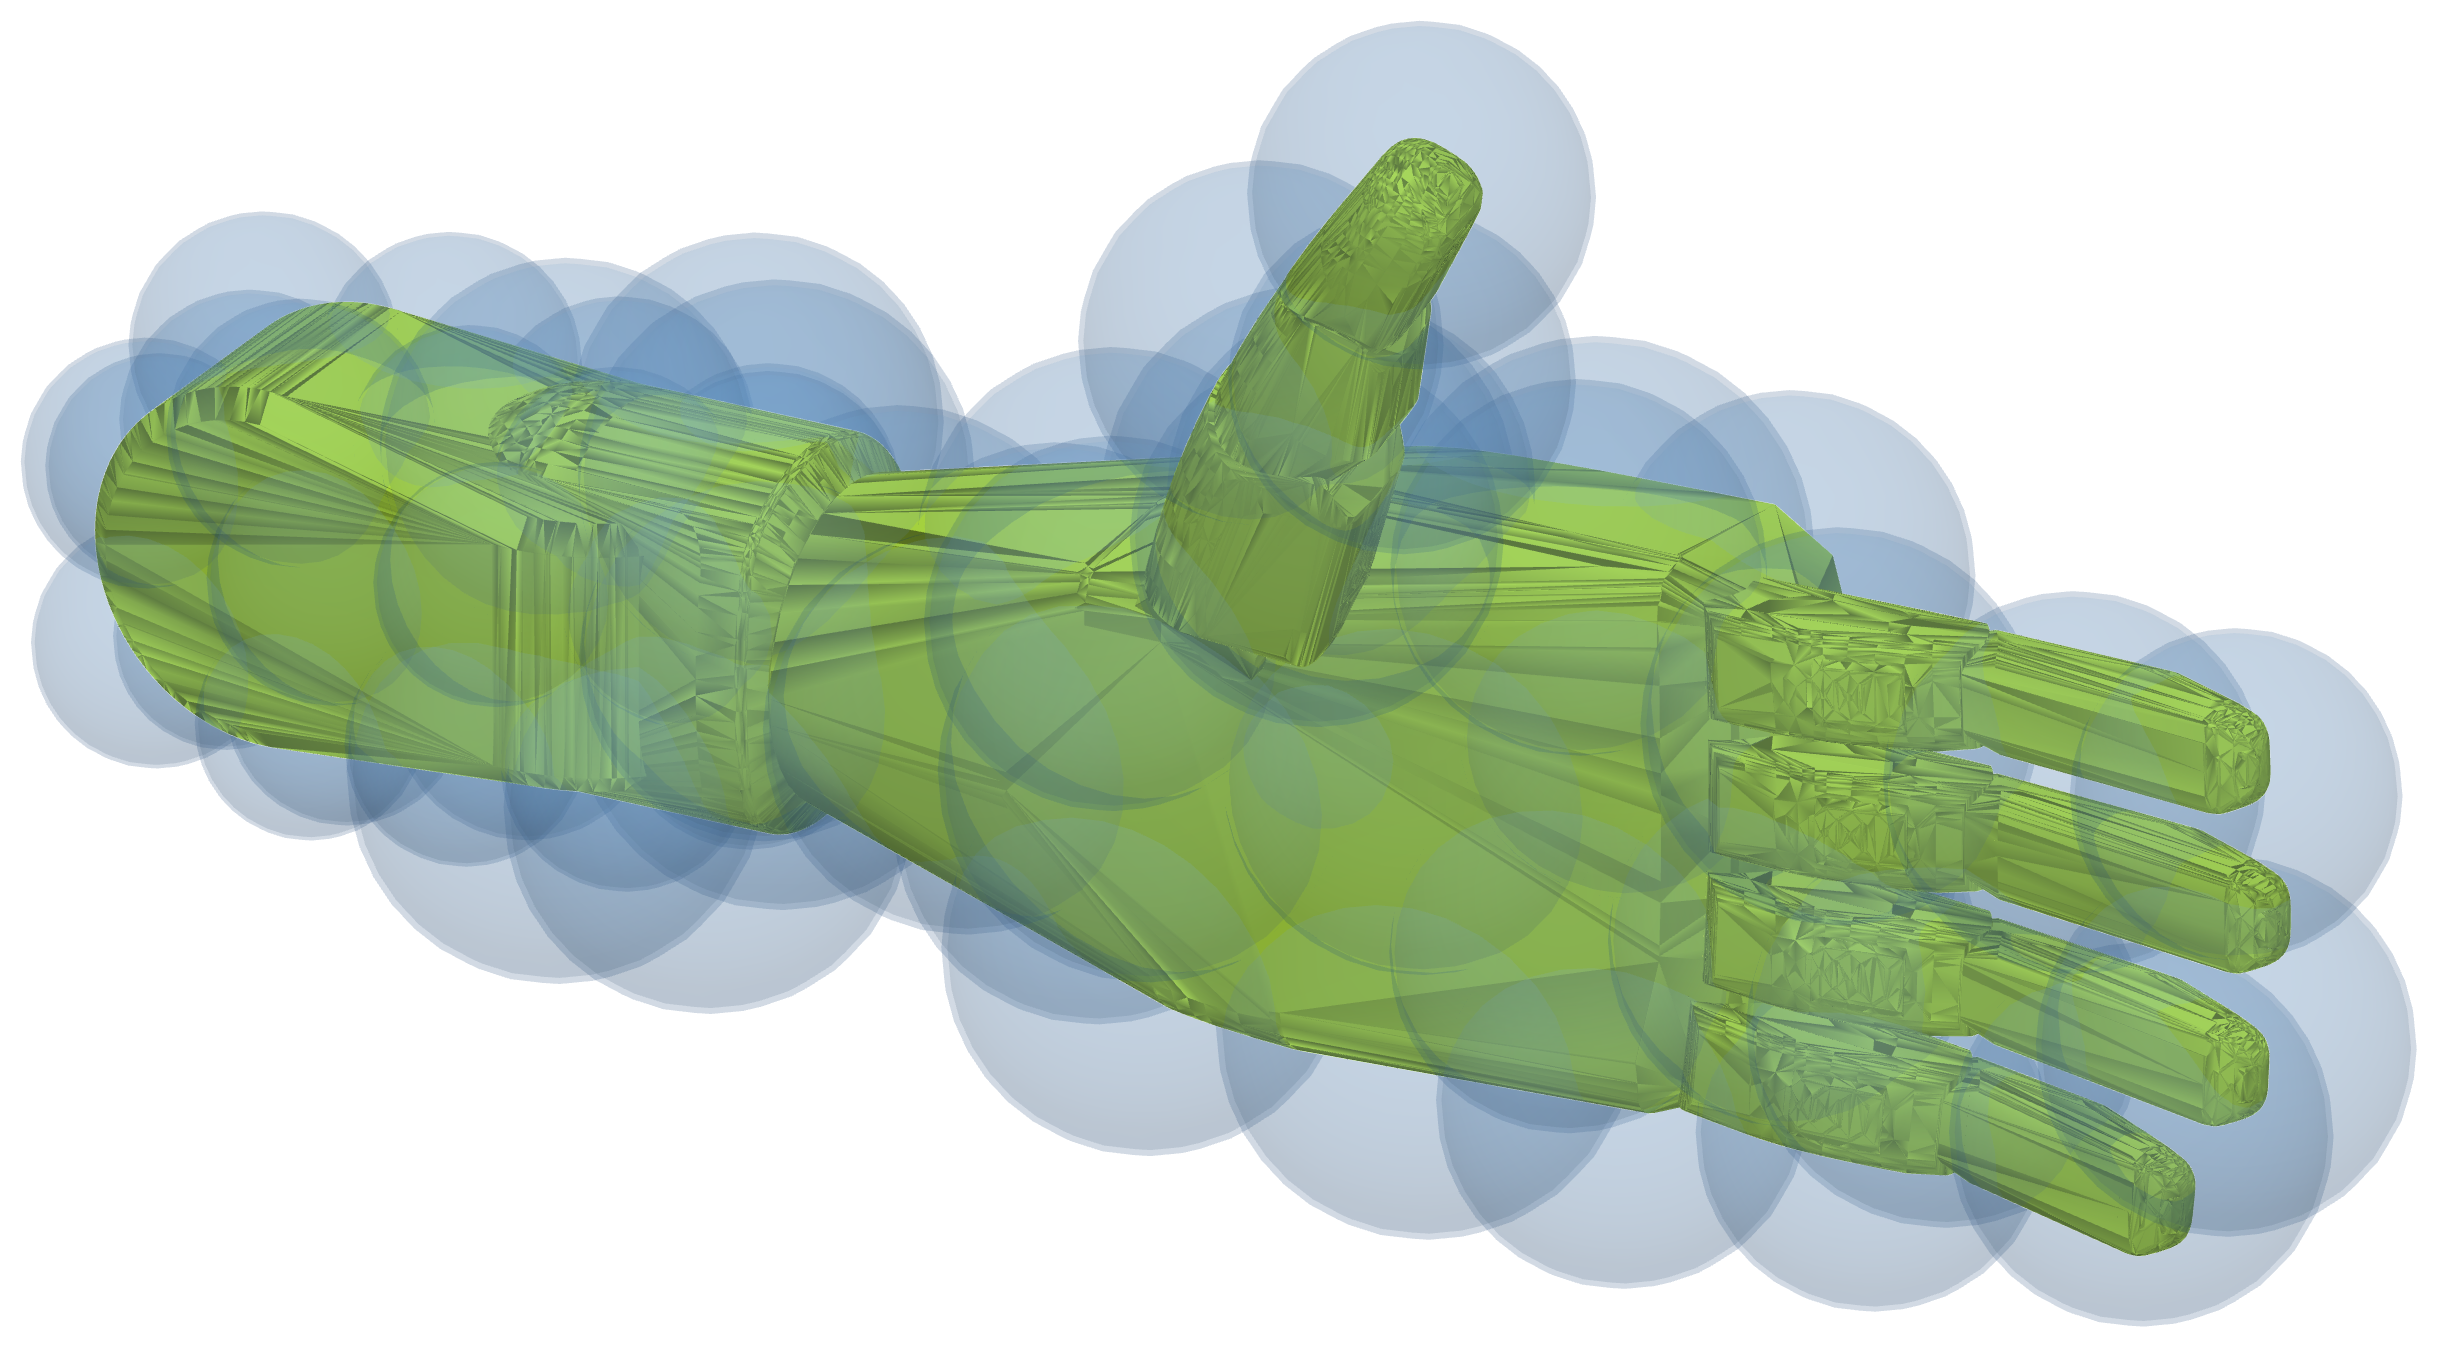
\includegraphics[width=14cm]{Bilder/kugelmodell-3d-inspire.png}};
  \node[ba teiltitel, anchor=north west] at ($(A.south west)+(0,-0.1)$) {a) Inspire-Hand (Modell auch für die Rubber Hand verwendet)};
  \node[anchor=north west, inner sep=0] (B) at ($(A.south west)+(0,-0.9)$) {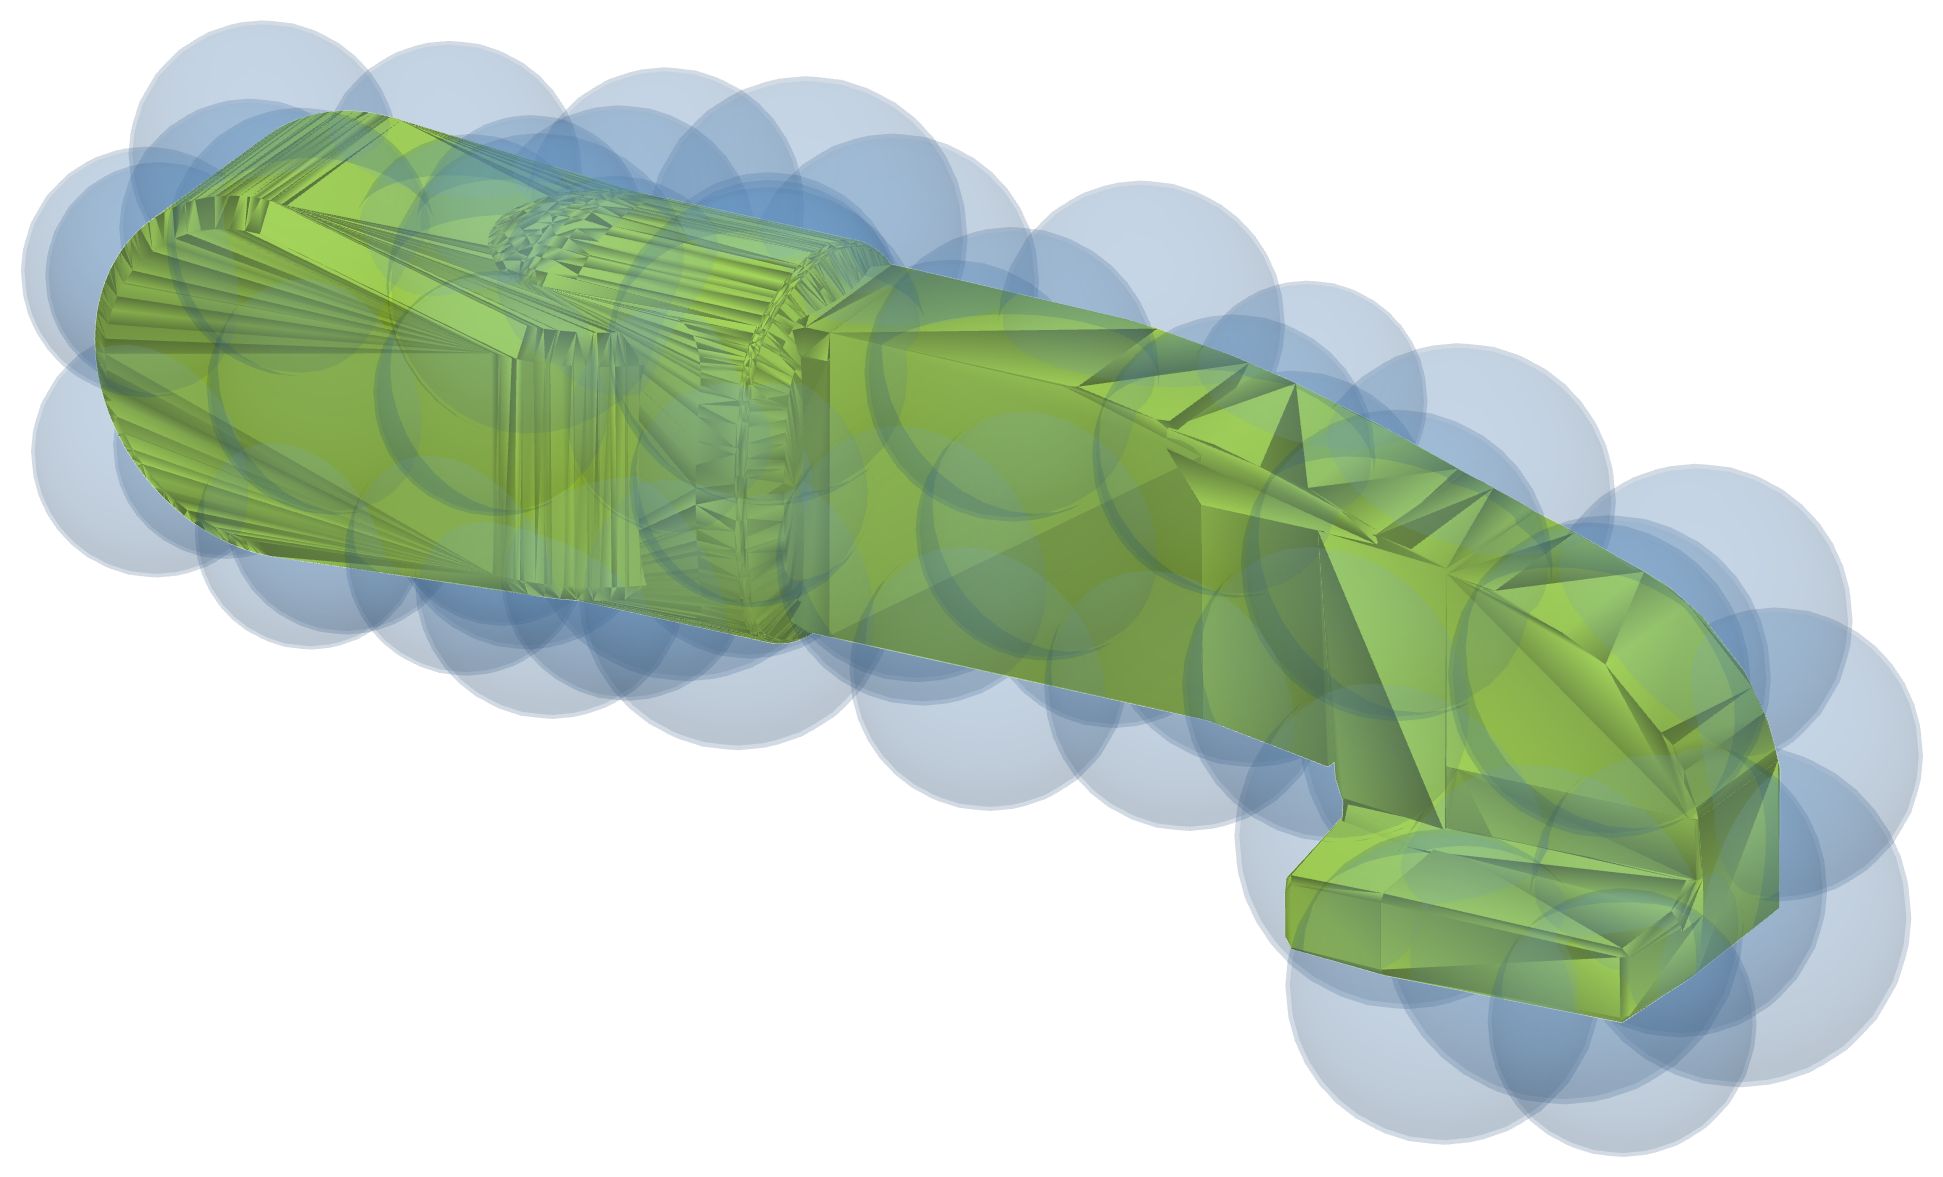
\includegraphics[width=11.16cm]{Bilder/kugelmodell-3d-haken.png}};
  \node[ba teiltitel, anchor=north west] at ($(B.south west)+(0,-0.1)$) {b) Gedruckter Box-Haken (Hand-Profil)};
  \fill[baGruen, draw=baGruen] ($(B.south west)+(0,-1.0)$) rectangle ++(0.4,0.3);
  \node[anchor=west] at ($(B.south west)+(0.45,-0.85)$) {Kollisionsgeometrie};
  \fill[baHellblau, fill opacity=0.45, draw=baBlau, draw opacity=0.5] ($(B.south west)+(4.4,-0.85)$) circle (0.17);
  \node[anchor=west] at ($(B.south west)+(4.65,-0.85)$) {Kugel des Planers};
\end{tikzpicture}

  \caption[Kugelmodell der Hand]{Kugelsatz der linken Hand für die Prüfung gegen die Umgebung. Die Kugeln umschließen die Kollisionsgeometrie der Hand und ragen deshalb über ihre Oberfläche hinaus.}
  \label{fig:kugelmodell}
\end{figure}

In beiden Teilbildern der Abbildung~\ref{fig:kugelmodell} stehen die Kugeln über die Handfläche hinaus.
Dieser Überstand bestimmt beim reaktiven Nachführen den kleinsten Abstand der Hand zu einer Fläche (Abschnitt~\ref{sec:laufzeitueberwachung}), seine Größe weist Abschnitt~\ref{sec:eval_manipulation} aus.
% DB: g1pilot/g1pilot/manipulation/arm_geometry.py:387-408,624-634 @e452513

% Abstände, Weltmodell, Greifobjekte, Sim/Real.
Objekte kennt das Modell als orientierte Quader aus dem gemeinsamen Weltmodell der Szene (Abschnitt~\ref{sec:szenen}).
Für jedes Paar aus Kugel und Quader liefert es den vorzeichenbehafteten Abstand der Oberflächen samt Gradient nach den Gelenkwinkeln, und zwar über eine eigene Vorwärtskinematik für viele Armstellungen zugleich.
Handkugeln dürfen Greifobjekte berühren, alle übrigen Kugeln nicht.
Weil das Weltmodell nur in der Simulation aus der Szene entsteht, prüft das Modell im Realbetrieb nur den eigenen Körper und die Arme gegeneinander \pruefen{Realbetrieb ohne Weltmodell so gewollt? Im Code startet die Szenenanbindung nur mit der Simulation}.
% DB: g1pilot/g1pilot/manipulation/arm_geometry.py:279-322,486-618 @e452513, g1pilot/g1pilot/manipulation/arm_planner.py:155-158 @e452513, unitree_mujoco/simulate_python/scene_objects.py:277-309 @e452513, g1pilot/launch/bringup_sim.launch.py:125-132 @e452513, g1pilot/g1pilot/navigation/scene_bridge.py:1-19,56 @e452513

\subsection{Bahnplaner}
\label{sec:bahnplaner}

% Rückbezug tab:schutzmechanismen (geplante Bahnen), Nutzer der geplanten Bewegung, Verweis auf Kap. 4.
Der Bahnplaner führt jede Armbewegung zu einem festen Ziel: gespeicherte Posen und Abläufe (Abschnitt~\ref{sec:posen_ablaeufe}), Ziele über die Arm-Schnittstelle (Abschnitt~\ref{sec:entwickler_api}), Grundstellung, Lauf-Pose und Rückgabe an den Onboard-Regler (Abschnitt~\ref{sec:armuebergabe}).
Seine Bahnen halten in der Mitte Abstand zu Objekten und führen nur nahe Start und Ziel dicht heran, weil die Hand dort oft auf einer Fläche aufliegt.
Die zugrunde liegenden Verfahren führt Abschnitt~\ref{sec:bahnplanung_sdt} ein.
% DB: g1pilot/g1pilot/manipulation/arm_planner.py:6-26 @e452513, g1pilot/g1pilot/manipulation/arm_controller.py:1382-1385,2363,2483-2486,2837,2862,2966 @e452513

% Leitidee Trichter, G7.6.
Dazu verlangt der Planer für jede Kugel~$k$ und jedes Objekt~$o$ einen Abstandsbedarf
\begin{equation}
  b_{ko} = f_{ko} + w_k\,\bigl(C - f_{ko}\bigr), \qquad
  w_k = 3u_k^2 - 2u_k^3, \qquad
  u_k = \min\left(\frac{a_k}{R},\ 1\right).
  \label{eq:abstandsbedarf}
\end{equation}
\formeleintrag{Abstandsbedarf des Bahnplaners mit Trichter um Start und Ziel}%
Darin ist $a_k$ der Abstand der Kugelmitte von ihrer Lage in der näheren der beiden Endstellungen, $R$ der Trichterradius und $C$ der Abstand in der Bahnmitte.
Der Endwert $f_{ko}$ ist der Abstand des Paars an diesem Endpunkt, wenn er negativ ist, und sonst null.
Liegt die Kugel nahe an beiden Endpunkten, gilt der kleinere Endwert, damit kurze Bewegungen auf einer Fläche lösbar bleiben \pruefen{Stand PR \#62, nach Merge BA-Stable-Hash eintragen}.
Voreingestellt sind $C = 5$\,cm und $R = 15$\,cm gegen die Umgebung sowie $C = 1{,}5$\,cm gegen Körper und anderen Arm.
% DB: g1pilot/g1pilot/manipulation/arm_planner.py:72-85,112-114,160-180,251-272,297-316 @e452513

Abbildung~\ref{fig:trichter} zeigt die Wirkung von Gleichung~\ref{eq:abstandsbedarf} an einer Handkugel.
Am Start liegt die Kugel auf, ihr Bedarf ist null.
Mit wachsendem $a_k$ steigt er ohne Knick bis zum vollen Abstand~$C$ bei $a_k = R$ und sinkt vor dem Ziel ebenso, sodass von selbst ein weicher Abhebe- und Anfahrbogen über das Hindernis entsteht.
Steckt eine Kugel am Endpunkt schon im Objekt (Teilbild~b), darf sie dort starten, aber nicht tiefer eindringen.
% DB: g1pilot/g1pilot/manipulation/arm_planner.py:13-26,251-272 @e452513, Daten/planer-trichter.py (Rechnung aus den Voreinstellungen)

\begin{figure}[htbp]
  \centering
  % Trichter des Armplaners: a) Skizze einer Handbahn über ein Hindernis mit dem Abstandsbedarf als Band,
% b) Abstandsbedarf über dem Abstand zum näheren Endpunkt (Gleichung eq:abstandsbedarf).
% Eigene Darstellung. a) schematisch, 1 cm in der Skizze = 10 cm; Band = Kugelradius + Bedarf b(a) mit
%   C = 5 cm, R = 15 cm, Endwert 0; Koordinaten der Bandränder einmalig mit derselben Formel berechnet
%   (kubische Bezierkurve (0.8,0.18) (0.8,2.4) (6.4,2.4) (6.4,0.18), Kugelradius 0.18).
% b) Daten: Daten/planer-trichter.csv aus Daten/planer-trichter.py (Voreinstellungen des Planers, kein Messwert).
% Code: G1 PR #62 @e452513, g1pilot/g1pilot/manipulation/arm_planner.py:72-100, 112-114, 251-272.
\begin{tikzpicture}[ba]
  % ---------------- a) Skizze ----------------
  \begin{scope}
    % Tisch und Hindernis (Flächen grau = Objekte des Weltmodells)
    \fill[baHellgrau] (0,-0.3) rectangle (7.2,0);
    \draw[baGrau, ba normal] (0,-0.3) rectangle (7.2,0);
    \fill[baHellgrau] (3.0,0) rectangle (4.2,1.0);
    \draw[baGrau, ba normal] (3.0,0) rectangle (4.2,1.0);
    \node[text=baGrau] at (3.6,0.5) {Hindernis};
    \node[text=baGrau, anchor=north] at (3.6,-0.32) {Tisch};
    % Band: Kugelradius + Abstandsbedarf entlang der Bahn
    \fill[baHellblau, fill opacity=0.35]
      (0.62,0.19) -- (0.62,0.37) -- (0.61,0.56) -- (0.62,0.75) -- (0.64,0.96) -- (0.69,1.17) -- (0.76,1.37) -- (0.87,1.57) -- (1.00,1.75) -- (1.17,1.91) -- (1.36,2.03) -- (1.56,2.13) -- (1.77,2.21) -- (1.98,2.29) -- (2.21,2.35) -- (2.43,2.41) -- (2.66,2.45) -- (2.89,2.48) -- (3.13,2.51) -- (3.36,2.52) -- (3.60,2.52) -- (3.84,2.52) -- (4.07,2.51) -- (4.31,2.48) -- (4.54,2.45) -- (4.77,2.41) -- (4.99,2.35) -- (5.22,2.29) -- (5.43,2.21) -- (5.64,2.13) -- (5.84,2.03) -- (6.03,1.91) -- (6.20,1.75) -- (6.33,1.57) -- (6.44,1.37) -- (6.51,1.17) -- (6.56,0.96) -- (6.58,0.75) -- (6.59,0.56) -- (6.58,0.37) -- (6.58,0.19)
      -- (6.22,0.17) -- (6.19,0.32) -- (6.13,0.44) -- (6.04,0.53) -- (5.93,0.60) -- (5.81,0.65) -- (5.68,0.68) -- (5.56,0.71) -- (5.44,0.74) -- (5.32,0.77) -- (5.21,0.83) -- (5.08,0.89) -- (4.95,0.94) -- (4.80,0.99) -- (4.65,1.04) -- (4.49,1.08) -- (4.32,1.11) -- (4.14,1.13) -- (3.96,1.15) -- (3.78,1.16) -- (3.60,1.16) -- (3.42,1.16) -- (3.24,1.15) -- (3.06,1.13) -- (2.88,1.11) -- (2.71,1.08) -- (2.55,1.04) -- (2.40,0.99) -- (2.25,0.94) -- (2.12,0.89) -- (1.99,0.83) -- (1.88,0.77) -- (1.76,0.74) -- (1.64,0.71) -- (1.52,0.68) -- (1.39,0.65) -- (1.27,0.60) -- (1.16,0.53) -- (1.07,0.44) -- (1.01,0.32) -- (0.98,0.17) -- cycle;
    \draw[baBlau, ba duenn, dash pattern=on 2pt off 1.5pt]
      (0.62,0.19) -- (0.62,0.37) -- (0.61,0.56) -- (0.62,0.75) -- (0.64,0.96) -- (0.69,1.17) -- (0.76,1.37) -- (0.87,1.57) -- (1.00,1.75) -- (1.17,1.91) -- (1.36,2.03) -- (1.56,2.13) -- (1.77,2.21) -- (1.98,2.29) -- (2.21,2.35) -- (2.43,2.41) -- (2.66,2.45) -- (2.89,2.48) -- (3.13,2.51) -- (3.36,2.52) -- (3.60,2.52) -- (3.84,2.52) -- (4.07,2.51) -- (4.31,2.48) -- (4.54,2.45) -- (4.77,2.41) -- (4.99,2.35) -- (5.22,2.29) -- (5.43,2.21) -- (5.64,2.13) -- (5.84,2.03) -- (6.03,1.91) -- (6.20,1.75) -- (6.33,1.57) -- (6.44,1.37) -- (6.51,1.17) -- (6.56,0.96) -- (6.58,0.75) -- (6.59,0.56) -- (6.58,0.37) -- (6.58,0.19);
    \draw[baBlau, ba duenn, dash pattern=on 2pt off 1.5pt]
      (6.22,0.17) -- (6.19,0.32) -- (6.13,0.44) -- (6.04,0.53) -- (5.93,0.60) -- (5.81,0.65) -- (5.68,0.68) -- (5.56,0.71) -- (5.44,0.74) -- (5.32,0.77) -- (5.21,0.83) -- (5.08,0.89) -- (4.95,0.94) -- (4.80,0.99) -- (4.65,1.04) -- (4.49,1.08) -- (4.32,1.11) -- (4.14,1.13) -- (3.96,1.15) -- (3.78,1.16) -- (3.60,1.16) -- (3.42,1.16) -- (3.24,1.15) -- (3.06,1.13) -- (2.88,1.11) -- (2.71,1.08) -- (2.55,1.04) -- (2.40,0.99) -- (2.25,0.94) -- (2.12,0.89) -- (1.99,0.83) -- (1.88,0.77) -- (1.76,0.74) -- (1.64,0.71) -- (1.52,0.68) -- (1.39,0.65) -- (1.27,0.60) -- (1.16,0.53) -- (1.07,0.44) -- (1.01,0.32) -- (0.98,0.17);
    % Bahn der Kugelmitte
    \draw[baBlau, ba normal] (0.8,0.18) .. controls (0.8,2.4) and (6.4,2.4) .. (6.4,0.18);
    % Trichterradius R um Start und Ziel
    \draw[ba hilfslinie] (0.8,0.18) ++(10:1.5) arc[start angle=10, end angle=125, radius=1.5];
    \draw[ba hilfslinie] (6.4,0.18) ++(55:1.5) arc[start angle=55, end angle=170, radius=1.5];
    \draw[ba duenn, baGrau, ->] (0.8,0.18) -- ++(125:1.5) node[midway, below left=-1pt, text=black] {$R$};
    \draw[ba duenn, baGrau, ->] (6.4,0.18) -- ++(55:1.5) node[midway, below right=-1pt, text=black] {$R$};
    % Abstandsbedarf C in der Bahnmitte
    \draw[ba duenn, black, <->] (3.6,2.03) -- (3.6,2.52);
    \node[anchor=west] at (3.65,2.36) {$C$};
    % Kugel der Hand an Start, Mitte, Ziel
    \foreach \p in {(0.8,0.18), (3.6,1.845), (6.4,0.18)}
      \fill[baGruen] \p circle (0.18);
    \node[anchor=north] at (0.8,-0.32) {Start};
    \node[anchor=north] at (6.4,-0.32) {Ziel};
    \node[ba teiltitel, anchor=north west] at (0,-1.55) {a) Bahn einer Handkugel mit Trichtern};
  \end{scope}
  % Trennlinie
  \draw[ba trenner] (7.55,-2.0) -- (7.55,3.0);
  % ---------------- b) Abstandsbedarf ----------------
  \begin{scope}[xshift=9.1cm, yshift=-0.3cm]
    \begin{axis}[ba plot, scale only axis, width=6.3cm, height=2.9cm,
        xmin=0, xmax=20, ymin=-2.5, ymax=6,
        xtick={0,5,10,15,20}, ytick={-2,0,2,4,6},
        xlabel={Abstand $a$ zum näheren Endpunkt in cm},
        ylabel={Bedarf $b$ in cm},
        legend pos=south east, legend style={font=\footnotesize}]
      \addplot+[no markers] table[x=a_cm, y=b_f0_cm, col sep=comma] {Daten/planer-trichter.csv};
      \addlegendentry{Endwert $f=0$}
      \addplot+[no markers, dash pattern=on 4pt off 2pt] table[x=a_cm, y=b_fm2_cm, col sep=comma] {Daten/planer-trichter.csv};
      \addlegendentry{Endwert $f=-2$\,cm}
      \draw[ba hilfslinie] (axis cs:15,-2.5) -- (axis cs:15,6);
      \node[anchor=south west, font=\footnotesize] at (axis cs:15,3.0) {$R$};
      \node[anchor=south west, font=\footnotesize] at (axis cs:0.5,5.0) {$C$};
    \end{axis}
    \node[ba teiltitel, anchor=north west] at (-1.55,-1.25) {b) Abstandsbedarf über dem Abstand};
  \end{scope}
\end{tikzpicture}

  \caption[Trichter des Bahnplaners]{Abstandsbedarf des Bahnplaners nach Gleichung~\ref{eq:abstandsbedarf} mit $C = 5$\,cm und $R = 15$\,cm. a) Schematische Bahn einer Handkugel (grün), das Band zeigt Kugelradius plus Bedarf. b) Berechneter Bedarf für zwei Endwerte, keine Messwerte.}
  \label{fig:trichter}
\end{figure}

% Optimierung, G7.7.
Die Bahn besteht aus 24 Stützpunkten im Gelenkraum zwischen fester Start- und Zielstellung, die gemeinsam die Kosten
\begin{equation}
  J(\xi) = \frac{1}{2}\,\xi^\mathsf{T} H\,\xi
  + \lambda_\mathrm{P} \sum_{t} \| p_{t+1} - p_t \|^2
  + \lambda_\mathrm{K} \sum_{t} \sum_{k,o} \max\bigl(0,\ b_{ko,t} - d_{ko,t}\bigr)^2
  + \lambda_\mathrm{A}\, J_\mathrm{A}
  \label{eq:planerkosten}
\end{equation}
\formeleintrag{Kostenfunktion der Bahnoptimierung}%
minimieren.
Darin enthält $\xi$ die Stützpunkte, $H$ ist die Glattheitsmatrix aus ersten und zweiten Differenzen, $p_t$ der Handpunkt, $d_{ko,t}$ der Abstand aus dem Kugelmodell, und die $\lambda$ sind Gewichte.
Der Term $J_\mathrm{A}$ lässt die Hand nahe an einem Objekt auf den letzten 10\,cm entlang ihrer Fingerrichtung ankommen, ersatzweise von oben.
Die Suchrichtung des Gradientenverfahrens ist mit $H^{-1}$ vorkonditioniert, sodass eine Korrektur an einer Stelle die ganze Bahn glatt verformt.
Diesen vorkonditionierten Gradientenabstieg nutzt auch CHOMP \cite{Schulman2014}\ev{Schulman2014.03}, er bevorzugt Änderungen mit wenig zusätzlicher Beschleunigung \cite{Zucker2013}\ev{Zucker2013.06}.
Bleibt am Ende eine Verletzung des Bedarfs, steigt $\lambda_\mathrm{K}$ stufenweise.
% DB: g1pilot/g1pilot/manipulation/arm_planner.py:86-88,102-109,194-245,356-464 @e452513

% Rückfallkette B7.10.
Weil die Optimierung in lokalen Minima hängen bleiben kann (Abschnitt~\ref{sec:bahnplanung_sdt}), durchläuft der Planer die Stufen in Abbildung~\ref{fig:rueckfallkette}, bis eine Bahn die Abschlussprüfung besteht.
Vorab lehnt er ein Ziel ab, das mit dem eigenen Körper kollidiert oder an der exakten Geometrie mehr als 2\,cm in ein Objekt eindringt.
Die vier Startbahnen der Optimierung sind die Gerade und Bögen, die die Hand um 15\,cm anheben, um 15\,cm zurückziehen und als letzter Versuch um 30\,cm anheben.
Danach sucht ein stichprobenbasierter Planer nach dem Prinzip von RRT-Connect \cite{Kuffner2000}\ev{Kuffner2000.01} mit dem kleinsten Abstand $C_\mathrm{min} = 1{,}5$\,cm, und die Glättung hebt den Abstand an, soweit die Bahn gültig bleibt.
Alle Stufen teilen sich 2,5\,s Rechenzeit.
\pruefen{Stand PR \#62, nach Merge BA-Stable-Hash eintragen: Zielprüfung an der exakten Geometrie, Startbahn 30\,cm}
% DB: g1pilot/g1pilot/manipulation/arm_planner.py:65-91,516-615,706-833 @e452513, g1pilot/g1pilot/manipulation/arm_geometry.py:621-696 @e452513, g1pilot/g1pilot/manipulation/arm_planner_process.py:53-58,115-125 @e452513

\begin{figure}[htbp]
  \centering
  % Rückfallkette des Armplaners: Zielprüfung, Gerade, Optimierung aus Startbahnen, stichprobenbasierter Planer,
% verringerter Abstand; jeder Versuch nur gültig nach bestandener Abschlussprüfung, danach Zeitparametrierung.
% Eigene Darstellung. Code: G1 PR #62 @e452513, g1pilot/g1pilot/manipulation/arm_planner.py:730-833 (_plan_arms),
% :483-501 (validate), :621-663 (time_parameterize).
% Stand PR #62 (vor Merge, nach Merge BA-Stable-Hash eintragen): Zielprüfung an der exakten Geometrie (:733-744),
% Startbahn "30 cm anheben" (:780-783).
\begin{tikzpicture}[ba, node distance=6mm,
    stufe/.style={ba block, minimum width=21mm, text width=19mm, minimum height=24mm, font=\footnotesize},
    ende/.style={ba block, minimum width=21mm, text width=19mm, minimum height=8mm, font=\footnotesize}]
  % Stufen in Prüfreihenfolge
  \node[stufe] (z) {\textbf{Vorab}\\ Zielprüfung: Kollision mit Körper, Eindringtiefe};
  \node[stufe, right=of z] (s1) {\textbf{Stufe 1}\\ Gerade im Gelenkraum};
  \node[stufe, right=of s1] (s2) {\textbf{Stufe 2}\\ Optimierung, vier Startbahnen, Abstand $C$};
  \node[stufe, right=of s2] (s3) {\textbf{Stufe 3}\\ RRT-Connect mit $C_\mathrm{min}$, dann Glättung};
  \node[stufe, right=of s3] (s4) {\textbf{Stufe 4}\\ kleinerer Abstand, auch über Lauf-Pose};
  \node[ende, right=of s4, draw=baAkzent, text=baAkzent] (nw) {kein Weg\\ gefunden};
  \node[ende, below=10mm of z, draw=baAkzent, text=baAkzent] (ab) {Ziel\\ abgelehnt};
  % Abbruchwege
  \draw[ba pfeil] (z) -- (s1);
  \draw[ba pfeil] (s1) -- (s2);
  \draw[ba pfeil] (s2) -- (s3);
  \draw[ba pfeil] (s3) -- (s4);
  \draw[ba pfeil] (s4) -- (nw);
  \draw[ba pfeil, baAkzent] (z) -- node[right, font=\footnotesize, align=left] {in\\ Kollision} (ab);
  \node[font=\footnotesize, text=baGrau, anchor=south west, inner xsep=0pt] at ([yshift=1mm]s1.north west) {Pfeil nach rechts: keine gültige Bahn, nächste Stufe};
  % Gemeinsamer Ausgang
  \coordinate (zpa) at ($(s1.south west)+(0,-8mm)$);
  \coordinate (zpb) at ($(s4.south east)+(0,-18mm)$);
  \draw[ba block hervor] (zpa) rectangle (zpb);
  \node[font=\footnotesize, align=center] (zp) at ($(zpa)!0.5!(zpb)$)
        {\textbf{Abschlussprüfung bestanden}\\ $\rightarrow$ Zeitparametrierung $\rightarrow$ Bahn an den Armregler};
  \foreach \s in {s1, s2, s3, s4}
    \draw[ba pfeil] (\s.south) -- (\s.south |- zpa);
\end{tikzpicture}

  \caption[Rückfallkette des Bahnplaners]{Rückfallkette des Bahnplaners. Die Stufen laufen von links nach rechts, bis ein Versuch die Abschlussprüfung besteht. $C$ ist der Abstand in der Bahnmitte, $C_\mathrm{min}$ der kleinste zulässige Abstand.}
  \label{fig:rueckfallkette}
\end{figure}

% Abschlussprüfung, Zeitparametrierung, Einbindung, Vorverweis.
Die Abschlussprüfung tastet jede Bahn dicht nach und prüft Bedarf, Gelenkgrenzen und die exakte Selbstkollision.
Die Zeitparametrierung begrenzt anschließend jedes Gelenk auf 1,2\,rad/s und 2\,rad/s$^2$ sowie jede Kugel und den Handpunkt auf 0,22\,m/s und 0,6\,m/s$^2$, also unter die Grenzen des Armreglers (Abschnitt~\ref{sec:regelkette}).
Unter 5\,cm Abstand zu einem Objekt sinkt das Tempo bis auf 35\,\%, damit die Hand sanft aufsetzt, in Simulation und Realbetrieb gleich.
Der Planer läuft in einem eigenen Prozess und plant beide Arme gemeinsam, und der Armregler verwirft ein Ergebnis, sobald eine neuere Anfrage oder ein Abbruch vorliegt.
Planungserfolg und Planungszeit weist Abschnitt~\ref{sec:eval_manipulation} aus.
% DB: g1pilot/g1pilot/manipulation/arm_planner.py:91-99,467-501,621-663 @e452513, g1pilot/g1pilot/manipulation/arm_controller.py:2969-2980,2982-3060,3062-3131,3148-3171 @e452513, g1pilot/g1pilot/manipulation/arm_planner_process.py:1-26 @e452513, g1pilot/launch/bringup_sim.launch.py:112 @e452513, g1pilot/launch/bringup_real.launch.py:106-107 @e452513

\subsection{Laufzeitüberwachung}
\label{sec:laufzeitueberwachung}

% Rückbezug tab:schutzmechanismen (Kollisionsprüfung zur Laufzeit), Stelle in der Regelkette.
Die Laufzeitüberwachung prüft in jedem Regeltakt den kommandierten Schritt der Arme, beim reaktiven Nachführen wie bei geplanten Bahnen.
Sie bildet die Kollisionsprüfung zur Laufzeit aus Tabelle~\ref{tab:schutzmechanismen}, sitzt hinter den Begrenzern für Geschwindigkeit und Beschleunigung (Abschnitt~\ref{sec:regelkette}) und schützt auch, wenn sich ein Objekt nach der Planung bewegt hat.
% DB: g1pilot/g1pilot/manipulation/arm_controller.py:1729-1761,3895-3908 @e452513

% Umgebung: Untergrenzen, Projektion G7.9, Verlangsamung.
Gegen Objekte gilt je Paar aus Kugel und Objekt eine Untergrenze von 0\,cm für Handkugeln, damit die Hand aufsetzen darf, und 1\,cm für die übrigen Armkugeln, gegenüber Greifobjekten gilt für Handkugeln keine.
Nähert sich ein Paar unter seiner Untergrenze weiter an, entfernt die Überwachung den annähernden Anteil aus dem Schritt
\begin{equation}
  \Delta q' = \Delta q - \frac{\min\bigl(0,\ g_{ko}^\mathsf{T}\Delta q\bigr)}{g_{ko}^\mathsf{T} g_{ko}}\, g_{ko}
  \label{eq:projektion}
\end{equation}
\formeleintrag{Projektion des Armschritts bei unterschrittener Untergrenze}%
mit dem Schritt $\Delta q$ der 14 Armgelenke und dem Gradienten $g_{ko}$ des Abstands nach den Gelenkwinkeln.
Die Hand gleitet so an der Fläche entlang, statt stehen zu bleiben.
Verletzt auch der projizierte Schritt eine Untergrenze, hält der Arm an.
Beim reaktiven Nachführen verkleinert die Überwachung außerdem Schritte, die sich einem Objekt auf weniger als 5\,cm über der Untergrenze nähern, bis auf 25\,\%.
% DB: g1pilot/g1pilot/manipulation/arm_controller.py:200-206,1623-1645,1663-1727,1740-1748 @e452513

% Selbstkollision.
Die Selbstkollision prüft die Überwachung exakt an den konvexen Hüllen von Ellbogen, Handgelenk und Handbasis gegen den Körper und den anderen Arm, die Finger bleiben zum Greifen ausgenommen.
Dafür nutzt sie das geometrische Modell der Starrkörperbibliothek Pinocchio mit Kollisions- und Abstandsberechnung auf Basis von FCL \cite{Carpentier2019}\ev{Carpentier2019.03,Carpentier2019.04}.
\qf{Kollisionsbibliothek coal (Nachfolger von hpp-fcl, von Pinocchio heute statt FCL genutzt) als GitHub-Quelle mit Commit-Hash}
Eine Durchdringung hält den Arm an, und ein Randband von 3\,cm darf nur eine geplante Bahn neu betreten, weil der Planer sie schon exakt geprüft hat.
% DB: g1pilot/g1pilot/utils/ik_solver.py:53,89,232-300,327-345 @e452513, g1pilot/g1pilot/manipulation/arm_controller.py:1603-1607,1750-1758 @e452513

% Gewolltes Berühren (L7.34), Bahnuhr, Sim/Real, Vorverweis.
Gewolltes Berühren regeln die Untergrenzen.
Während einer geplanten Bewegung sinken sie auf die Werte an Start und Ziel der Bahn abzüglich 3\,mm, sodass die Bewegung mit aufliegender Hand enden darf \pruefen{Stand PR \#62: erst mit der exakten Zielprüfung liegt die Hand wirklich auf}.
Das reaktive Nachführen hält dagegen schon an, wenn das Kugelmodell die Fläche erreicht, also etwas über ihr.
Hält die Überwachung eine geplante Bewegung an, steht auch deren Bahnuhr, und nach 3\,s Stillstand bricht die Bewegung ab.
Die Werte gelten in Simulation und Realbetrieb gleich, die Prüfung gegen Objekte wirkt aber nur in der Simulation (Abschnitt~\ref{sec:kollisionsmodell}).
Die Prüfung der Schutzmechanismen beschreibt Abschnitt~\ref{sec:eval_sicherheit}.
% DB: g1pilot/g1pilot/manipulation/arm_controller.py:1623-1645,3115-3124,3735-3795 @e452513, g1pilot/g1pilot/manipulation/arm_geometry.py:624-638 @e452513, g1pilot/launch/manipulation_launcher.launch.py:32,36 @e452513, g1pilot/launch/bringup_real.launch.py:108 @e452513

\section{Roboterhände}
\label{sec:haende}
Am G1 bindet die Umgebung die Inspire-Hände an und erlaubt in der Simulation, sie gegen eigene Handformen wie einen Haken zu tauschen.
Abbildung~\ref{fig:haende} zeigt beide Ausführungen.
Die Inspire-Hand ist in Simulation und Realbetrieb verfügbar und über eine gemeinsame Schnittstelle ansprechbar (Abschnitt~\ref{sec:hand_schnittstelle}).
Eigene Handformen beschreibt ein austauschbares Hand-Profil, das nur in der Simulation wirkt (Abschnitt~\ref{sec:hand_profile}).
% DB: g1pilot/g1pilot/manipulation/inspire_ftp/bridge.py:45-85 @6a40e47, g1pilot/g1pilot/utils/hand_profile.py:1-79 @6a40e47

\begin{figure}[htbp]
  \centering
  \begin{minipage}[t]{0.48\textwidth}
    \centering
    \fbox{\parbox[c][5cm][c]{0.9\textwidth}{\centering Platzhalter: Inspire-Hand am G1}}\\[1mm]
    {\small a) Inspire-Hand}
  \end{minipage}\hfill
  \begin{minipage}[t]{0.48\textwidth}
    \centering
    \fbox{\parbox[c][5cm][c]{0.9\textwidth}{\centering Platzhalter: Haken am G1}}\\[1mm]
    {\small b) Haken als eigenes Hand-Profil}
  \end{minipage}
  \caption[Handausführungen am G1]{Handausführungen am G1: a) Inspire-Hand, b) Haken als eigenes Hand-Profil.}
  \label{fig:haende}
\end{figure}
\pruefen{Bild von Nils: Bilder/kap7/hand-inspire.jpg}

\pruefen{Bild von Nils: Bilder/kap7/hand-haken.jpg}

Der Haken besteht aus zwei gedruckten, starren Teilen ohne bewegliche Finger, eines je Hand.
Er wiegt nach Schätzung rund 110\,g \pruefen{Schätzwert von Nils (110\,g, nicht gewogen): je Hand oder für beide? Das Hand-Profil trägt 0,15\,kg je Hand, bitte wiegen und Text und Profil angleichen}.
% DB: unitree_mujoco/unitree_robots/g1/hands/haken/hand.yaml:1-16 @6a40e47

\subsection{Schnittstelle der Inspire-Hände}
\label{sec:hand_schnittstelle}
% Basis: Code inspire_ftp/{joint_map,backends,bridge,model}.py; Model g1_29dof_inspire_ftp.xml.
Die Hände sind ein eigener Andockpunkt der Umgebung (Abschnitt~\ref{sec:andockpunkte}), den Simulation und Realbetrieb mit derselben Schnittstelle bedienen (Abschnitt~\ref{sec:haende_sdt}).
Jede Hand hat 12 Gelenke, aber nur 6 Freiheitsgrade, und 6 Kraftsensoren \cite{Inspire2024}\ev{Inspire2024.03}.
Jeder Freiheitsgrad nimmt einen Winkelwert von 0 bis 1000 an \cite{Inspire2024}\ev{Inspire2024.07}.
Der Wert 1000 steht für den ganz geöffneten Finger \cite{Inspire2024}\ev{Inspire2024.09}, und die Umgebung bildet jeden dieser Werte auf die gekoppelten Gelenke ab.
Die Schnittstelle läuft mit 50\,Hz, nimmt Fingerziele aus Posen und Bedienoberfläche an und gibt Winkel, Kräfte und Taktilwerte als Gelenkzustand zurück.
% DB: g1pilot/g1pilot/manipulation/inspire_ftp/joint_map.py:1-61 @6a40e47, g1pilot/g1pilot/manipulation/inspire_ftp/bridge.py:45,49,195-208 @6a40e47

Hinter der Schnittstelle stehen drei austauschbare Anbindungen, die Tabelle~\ref{tab:hand_anbindungen} vergleicht.

\begin{table}[htbp]
  \tabstil
  \centering
  \caption[Anbindungen der Inspire-Hände]{Anbindungen der Inspire-Hände hinter der gemeinsamen Schnittstelle.}
  \label{tab:hand_anbindungen}
  \begin{tabularx}{\textwidth}{|>{\raggedright\arraybackslash}p{2.4cm}|L|L|L|}\hline
    \tabkopfzeile \tabkopf{Anbindung} & \tabkopf{Fingerbewegung} & \tabkopf{Kraft und Taktilwerte} & \tabkopf{Einsatz}\\\hline
    Nur Anzeige & folgt dem Sollwert mit begrenzter Geschwindigkeit, ohne Physik & keine, Kraft immer null & Simulation, wahlweise\\\hline
    Kontaktphysik & je Hand 12 Positionsservos im Physikmodell bewegen die Finger & 17 Taktilzonen je Hand, Kraft je Finger als Summe ihrer Zonen, Kraftgrenze durch Rückstellung des Winkels & Simulation, Standard\\\hline
    Modbus TCP & Register der realen Hand, Sollwerte nur bei Änderung & Lesen mit 20\,Hz, Taktilwerte in jedem zweiten Zyklus, Kraftgrenze in der Hand & Realbetrieb, Standard\\\hline
  \end{tabularx}
\end{table}
% DB: g1pilot/g1pilot/manipulation/inspire_ftp/backends.py:51-108,111-387,390-515,518-564 @6a40e47, g1pilot/launch/bringup_sim.launch.py:171-183 @6a40e47, g1pilot/launch/bringup_real.launch.py:197-210 @6a40e47, unitree_mujoco/simulate_python/unitree_sdk2py_bridge.py:61-90,403-416 @6a40e47

Die Kontaktphysik ist in der Simulation voreingestellt.
Sie bewegt die Finger über Positionsservos, deren Verstärkung das Physikmodell festlegt \cite{MujocoDoku2026b}\ev{MujocoDoku2026b.02}, und misst den Kontakt mit Berührungssensoren \cite{MujocoDoku2026a}\ev{MujocoDoku2026a.08}.
Übersteigt die Kraft eines Fingers die eingestellte Grenze, voreingestellt 500\,g, öffnet die Anbindung ihn im Verhältnis zur Überschreitung und hält ihn an der erreichten Stelle.
Damit bildet sie das Verhalten der realen Hand nach, deren Greifkraft sich über Kraftschwellen einstellen lässt \cite{Inspire2024}\ev{Inspire2024.01}.
In der Anleitung des Herstellers hält etwa der Zeigefinger an, sobald die gemessene Kraft beim Beugen den Wert 300 erreicht \cite{Inspire2024}\ev{Inspire2024.08}.
% DB: g1pilot/g1pilot/manipulation/inspire_ftp/backends.py:111-387 @6a40e47, g1pilot/g1pilot/manipulation/inspire_ftp/model.py:18-35 @6a40e47

Im Realbetrieb spricht die Anbindung die Hände über Modbus TCP an, das die Hand über IP-Adresse und Port steuert \cite{Inspire2024}\ev{Inspire2024.06}.
Sie liest die Istwerte mit 20\,Hz in einem eigenen Ablauf je Hand, damit eine langsame oder getrennte Verbindung den Takt der Anbindung nicht blockiert.
Ein Not-Halt schaltet in Simulation und Realbetrieb beide Hände ab, und die reale Hand bekommt dabei ihren gemessenen Winkel als Ziel, sodass sie stehen bleibt.
Wie die Hände am realen Roboter greifen, zeigt Abschnitt~\ref{sec:eval_realtests}.
% DB: g1pilot/g1pilot/manipulation/inspire_ftp/backends.py:390-515 @6a40e47, g1pilot/g1pilot/manipulation/inspire_ftp/bridge.py:80-85,251-258 @6a40e47

\subsection{Austauschbare Hand-Profile}
\label{sec:hand_profile}
% Basis: Code unitree_mujoco/unitree_robots/g1/tools/gen_hand_profile.py, g1pilot/g1pilot/utils/hand_profile.py, g1pilot/start.sh.
Austauschbare Hand-Profile sind eine reine Simulationsfunktion, mit der sich andere Endeffektoren am Modell des G1 erproben lassen (Abschnitt~\ref{sec:andockpunkte}).
Am realen Roboter verwendet die Umgebung immer das Modell der Inspire-Hand, auch wenn ein anderes Profil gewählt ist.
Ein Profil besteht aus einer Beschreibungsdatei und einem Netz der Handform. Ein Generator erzeugt daraus alle Modelle, die die Umgebung braucht.
Abbildung~\ref{fig:handprofil} zeigt diesen Ablauf.
% DB: g1pilot/g1pilot/utils/hand_profile.py:1-79 @6a40e47, unitree_mujoco/unitree_robots/g1/tools/gen_hand_profile.py:1-28 @6a40e47

\begin{figure}[htbp]
  \centering
  % Ablauf eines Hand-Profils (B7.11, fig:handprofil, Abschnitt sec:hand_profile). Nur Simulation.
% Eigene Darstellung (Eigenleistung), keine Quelle in der Caption.
% Datenbasis G1@6a40e47 (BA-Stable), Pfade relativ zur Repo-Wurzel:
%   Profil: unitree_mujoco/unitree_robots/g1/hands/haken/hand.yaml:1-37 (Beschreibung + STL).
%   Generator: unitree_mujoco/unitree_robots/g1/tools/gen_hand_profile.py:154-190 (Abbildung, Gl. eq:handabbildung),
%     :193-220 (konvexe Zerlegung), :222-236 (Trägheit), :71-83 (Prüfsumme), :437-441 (Prüfung beim Start),
%     g1pilot/start.sh:341-353 (Neuerzeugen beim Start).
%   Ausgaben: gen_hand_profile.py:319-371 (MJCF + Szene), :372-436 (URDF mit Kollisionsteilen und Werkzeugpunkt).
%   Nutzer: Simulation (MJCF), g1pilot/g1pilot/navigation/loco_sim.py:331-345 (Schwerpunktmodell Ersatzregler),
%     g1pilot/g1pilot/utils/ik_solver.py:237-238 (IK/Anzeige über URDF), g1pilot/g1pilot/manipulation/arm_geometry.py:36-46,370-400
%     (Kugelmodell aus der Kollisionsgeometrie).
% Stil: ba-grafik.tex. Nicht skalieren.
\begin{tikzpicture}[ba]
  \tikzset{
    hp/.style={ba block, text width=30mm, minimum height=10mm},
    gen/.style={ba block hervor, text width=38mm, minimum height=27mm},
    sp/.style={font=\footnotesize, text=baGrau, anchor=south},
  }
  % Spaltenköpfe
  \node[sp] at (1.75,1.75) {Profil};
  \node[sp] at (6.0,1.75) {Generator};
  \node[sp] at (10.15,1.75) {Modelle};
  \node[sp] at (14.25,1.75) {Nutzer};
  % Profil
  \node[hp] (BE) at (1.75,0.75) {Beschreibung\\(Montage, Masse)};
  \node[hp] (NE) at (1.75,-0.75) {Netz der\\Handform};
  % Generator
  \node[gen, align=left] (GE) at (6.0,0) {Abbildung in das\\Handgelenk\\(Gleichung~\ref{eq:handabbildung})\\[1mm]
    konvexe Zerlegung\\[1mm] Trägheit\\[1mm] Prüfsumme};
  % Modelle
  \node[hp] (PM) at (10.15,0.75) {Physikmodell\\mit Szene};
  \node[hp] (KM) at (10.15,-0.75) {Kinematikmodell\\mit Kollisions\-teilen};
  % Nutzer
  \node[hp, minimum height=7mm, font=\footnotesize] (U1) at (14.25,1.35) {Simulation};
  \node[hp, minimum height=7mm, font=\footnotesize] (U2) at (14.25,0.45) {Schwerpunktmodell};
  \node[hp, minimum height=7mm, font=\footnotesize] (U3) at (14.25,-0.45) {Kinematik, Anzeige};
  \node[hp, minimum height=7mm, font=\footnotesize] (U4) at (14.25,-1.35) {Kollisionsmodell};
  % Pfeile
  \draw[ba pfeil] (BE.east) -- (BE.east -| GE.west);
  \draw[ba pfeil] (NE.east) -- (NE.east -| GE.west);
  \draw[ba pfeil] (GE.east |- PM.west) -- (PM.west);
  \draw[ba pfeil] (GE.east |- KM.west) -- (KM.west);
  \draw[ba pfeil] (PM.east) -- (U1.west);
  \draw[ba pfeil] (PM.east) -- (U2.west);
  \draw[ba pfeil] (KM.east) -- (U3.west);
  \draw[ba pfeil] (KM.east) -- (U4.west);
\end{tikzpicture}

  \caption[Ablauf eines Hand-Profils]{Ablauf eines Hand-Profils vom Netz der Handform bis zu den Nutzern in der Simulation.}
  \label{fig:handprofil}
\end{figure}

Der Generator legt das Netz zuerst in das Koordinatensystem des Handgelenks.
Dafür gibt die Beschreibung an, welche Richtung der Handform vom Arm weg und welche zur Handfläche zeigt.
Daraus folgt nach Gleichung~\ref{eq:handabbildung} die Abbildung jedes Netzpunkts
\begin{equation}
  \mathbf{p}_\mathrm{w} = \mathbf{A}\,\mathbf{p}_\mathrm{s} + \mathbf{b}
  \quad\mathrm{mit}\quad
  \mathbf{A} = s\,\mathbf{H}\,\mathbf{R}\,\mathbf{Q}^\mathrm{T}\mathbf{M} ,
  \quad
  \mathbf{b} = \mathbf{f} + \mathbf{H}\,\mathbf{d} - \mathbf{A}\,\mathbf{o} ,
  \label{eq:handabbildung}
\end{equation}
\formeleintrag{Abbildung eines Hand-Profils in das Handgelenk}%
wobei $\mathbf{p}_\mathrm{s}$ ein Punkt des Netzes ist und $\mathbf{p}_\mathrm{w}$ derselbe Punkt im Koordinatensystem des Handgelenks.
$\mathbf{Q}$ fasst die angegebenen Richtungen der Handform zusammen und $\mathbf{H}$ dieselben Richtungen am Handgelenk, wobei die Handfläche links und rechts zueinander gespiegelt liegt.
$\mathbf{R}$ ist eine optionale Feindrehung, $s$ der Maßstab des Netzes und $\mathbf{M}$ eine Spiegelung für die linke Hand, sonst die Einheitsmatrix.
$\mathbf{o}$ ist der Ursprung im Netz, $\mathbf{f}$ der Mittelpunkt des Flansches 41,5\,mm vor dem Handgelenk und $\mathbf{d}$ ein optionaler Versatz.
Damit genügt ein einziges Netz für beide Hände.
% DB: unitree_mujoco/unitree_robots/g1/tools/gen_hand_profile.py:53,154-190 @6a40e47, unitree_mujoco/unitree_robots/g1/hands/haken/hand.yaml:19-37 @6a40e47

Weil die Kollisionserkennung des Physikmodells mit der konvexen Hülle eines Netzes arbeitet \cite{MujocoDoku2026a}\ev{MujocoDoku2026a.10}, zerlegt der Generator die Handform in mehrere konvexe Teile \qf{Beleg für das Verfahren der näherungsweisen konvexen Zerlegung (V-HACD)}.
Die Trägheit berechnet er aus dem Netz bei gleichmäßiger Dichte und der Masse aus der Beschreibung, die ein Dialog der Bedienoberfläche beim Anlegen einer neuen Hand aus dem Volumen schätzt.
Aus Profil und Generator bildet er eine Prüfsumme und erzeugt beim Start neu, sobald sie nicht mehr passt. Lässt sich ein Profil nicht bauen, startet die Umgebung mit einem mitgelieferten Standardprofil.
% DB: unitree_mujoco/unitree_robots/g1/tools/gen_hand_profile.py:54-83,193-236,437-441 @6a40e47, unitree_mujoco/unitree_robots/g1/tools/hand_new.py:1-17,38-39,66-69 @6a40e47, g1pilot/start.sh:341-353 @6a40e47

Der Generator liefert ein Physikmodell mit Szene und ein Kinematikmodell mit Kollisionsteilen und Werkzeugpunkt.
Das Physikmodell nutzen die Simulation und das Schwerpunktmodell des Ersatzreglers, das Kinematikmodell die inverse Kinematik, die Anzeige und das Kollisionsmodell (Abschnitt~\ref{sec:kollisionsmodell}).
Ein neues Profil wirkt so ohne Änderung am Code auf Simulation, Stehen, inverse Kinematik und Kollisionsprüfung.
Wie sich die Umgebung damit um eigene Endeffektoren erweitern lässt, ordnet Abschnitt~\ref{sec:eval_modular} ein.
Die Bedienschritte zum Anlegen eines Profils stehen in Anhang~\ref{anh:dokumentation}.
% DB: unitree_mujoco/unitree_robots/g1/tools/gen_hand_profile.py:242-298,319-436 @6a40e47, g1pilot/g1pilot/navigation/loco_sim.py:331-345 @6a40e47, g1pilot/g1pilot/manipulation/arm_geometry.py:36-46,370-400 @6a40e47, g1pilot/g1pilot/utils/ik_solver.py:237-238 @6a40e47

% Paket D (Kap. Umsetzung): 7.6 Bedienwege mit 7.6.1 bis 7.6.4. Entwurf 27.11.2026, Code-Stand G1 BA-Stable @6a40e47.
% Direkt in Kapitel/07_Umsetzung.tex einfügbar (ersetzt das Gerüst von \section{Bedienwege} bis vor \section{Navigation in der Simulation}).
% Pfade in % DB: relativ zur Repo-Wurzel des Code-Repos (G1 / g1-ba).
\section{Bedienwege}
\label{sec:bedienwege}
Alle Bedienwege erzeugen nur Befehle auf gemeinsamen Befehlsthemen, sodass Bewegungslogik und Schutzmechanismen in den Zielprogrammen liegen und sich von keinem Bedienweg umgehen lassen (Abschnitt~\ref{sec:bedienwege_konzept}).
Abbildung~\ref{fig:bedienwege_signal} zeigt den Signalweg von der Eingabe bis zur Herstellerschnittstelle, und Tabelle~\ref{tab:bedienwege_umsetzung} nennt je Bedienweg das Eingabegerät, die Schnittstelle zum System und die Auslegungswerte der Zeitüberwachung.
Der Funktionsumfang je Bedienweg steht in Tabelle~\ref{tab:bedienwege}, die Wirkprinzipien der Schutzmechanismen in Tabelle~\ref{tab:schutzmechanismen}.
% DB: g1pilot/docs/10-T-Demo-GUI.md (Grundsatz), g1pilot/g1pilot/teleoperation/demo_gui.py:1143 (Anbindung des Smartphones an die Bedienoberfläche), g1pilot/g1pilot/manipulation/arm_api.py:3-30 (Brücke ohne Regellogik)

\begin{figure}[htbp]
  \centering
  % Signalfluss der Bedienwege: Eingabe, Bedienprogramm, gemeinsame Befehlsthemen, Zielprogramme, Herstellerschnittstelle.
% Eigene Darstellung (Abschnitt "Bedienwege" in Kapitel Umsetzung, B7.13). Keine Quelle in der Caption.
% Basis: G1@6a40e47 g1pilot/docs/10-T-Demo-GUI.md (Grundsatz, Topics), docs/11-T-Controller.md (Datenfluss),
%   docs/12-T-Handy.md (Aufbau: Vermittlungsschicht im Prozess der Bedienoberfläche), docs/21-T-Arm-API.md (Architektur, direkter DDS-Zugang),
%   g1pilot/manipulation/interactive_marker.py (Zielmarker), g1pilot/teleoperation/phone/link.py (Anbindung an die GUI-Methoden).
% Vereinfachungen: Hände real über Modbus (siehe fig:sim_real_schalter), Navigation in der Simulation und Posenspeicher nicht gezeichnet.
% Stil: ba-grafik.tex. Einbinden: % Signalfluss der Bedienwege: Eingabe, Bedienprogramm, gemeinsame Befehlsthemen, Zielprogramme, Herstellerschnittstelle.
% Eigene Darstellung (Abschnitt "Bedienwege" in Kapitel Umsetzung, B7.13). Keine Quelle in der Caption.
% Basis: G1@6a40e47 g1pilot/docs/10-T-Demo-GUI.md (Grundsatz, Topics), docs/11-T-Controller.md (Datenfluss),
%   docs/12-T-Handy.md (Aufbau: Vermittlungsschicht im Prozess der Bedienoberfläche), docs/21-T-Arm-API.md (Architektur, direkter DDS-Zugang),
%   g1pilot/manipulation/interactive_marker.py (Zielmarker), g1pilot/teleoperation/phone/link.py (Anbindung an die GUI-Methoden).
% Vereinfachungen: Hände real über Modbus (siehe fig:sim_real_schalter), Navigation in der Simulation und Posenspeicher nicht gezeichnet.
% Stil: ba-grafik.tex. Einbinden: % Signalfluss der Bedienwege: Eingabe, Bedienprogramm, gemeinsame Befehlsthemen, Zielprogramme, Herstellerschnittstelle.
% Eigene Darstellung (Abschnitt "Bedienwege" in Kapitel Umsetzung, B7.13). Keine Quelle in der Caption.
% Basis: G1@6a40e47 g1pilot/docs/10-T-Demo-GUI.md (Grundsatz, Topics), docs/11-T-Controller.md (Datenfluss),
%   docs/12-T-Handy.md (Aufbau: Vermittlungsschicht im Prozess der Bedienoberfläche), docs/21-T-Arm-API.md (Architektur, direkter DDS-Zugang),
%   g1pilot/manipulation/interactive_marker.py (Zielmarker), g1pilot/teleoperation/phone/link.py (Anbindung an die GUI-Methoden).
% Vereinfachungen: Hände real über Modbus (siehe fig:sim_real_schalter), Navigation in der Simulation und Posenspeicher nicht gezeichnet.
% Stil: ba-grafik.tex. Einbinden: \input{Bilder/tikz/bedienwege-signalfluss} in einer figure-Umgebung. Nicht skalieren.
% Raster (cm): Zeilenabstand 1,45, Blockhöhe 1,15. Spalten: Eingabe 0..2,9 | Bedienprogramm 3,5..6,9 | Befehlsthemen 7,5..10,6 | Zielprogramme 11,3..15,0.
\begin{tikzpicture}[ba]
  \tikzset{
    ein/.style={ba block, font=\footnotesize, minimum width=29mm, minimum height=11.5mm, text width=26mm},
    prog/.style={ba block hervor, font=\footnotesize, minimum width=34mm, minimum height=11.5mm, text width=31mm},
    thema/.style={ba block, font=\footnotesize, minimum width=27mm, minimum height=10mm, text width=25mm, inner sep=2pt},
    ziel/.style={ba block hervor, font=\footnotesize, minimum width=31mm, minimum height=14mm, text width=28mm},
    kopf/.style={font=\footnotesize, text=baGrau, anchor=north, align=center},
  }
  % ---------------- Spaltenköpfe ----------------
  \node[kopf] at (1.45,1.85) {Eingabe};
  \node[kopf] at (5.2,1.85)  {Bedienprogramm};
  \node[kopf] at (9.05,1.85) {Befehlsthemen};
  \node[kopf] at (13.15,1.85) {Zielprogramme mit\\Schutzmechanismen};
  % ---------------- Eingabe und Bedienprogramme (Zeilen y = 0, -1,45, ... -5,8) ----------------
  \node[ein]  (E1) at (1.45,0)     {Bildschirm,\\Maus};
  \node[ein]  (E2) at (1.45,-1.45) {Smartphone\\(Browser, BLE)};
  \node[ein]  (E3) at (1.45,-2.9)  {Controller\\(USB, Bluetooth)};
  \node[ein]  (E4) at (1.45,-4.35) {RViz\\(Maus)};
  \node[ein]  (E5) at (1.45,-5.8)  {Fremdes Programm\\(HTTP)};
  \node[ein]  (E6) at (1.45,-8.1)  {Fremdes Programm\\(DDS)};
  \node[prog] (P1) at (5.2,0)      {Bedienoberfläche};
  \node[prog] (P2) at (5.2,-1.45)  {Vermittlungsschicht};
  \node[prog] (P3) at (5.2,-2.9)   {Controller-Programme};
  \node[prog] (P4) at (5.2,-4.35)  {Zielmarker};
  \node[prog] (P5) at (5.2,-5.8)   {HTTP-Brücke};
  % Bedienoberfläche und Vermittlungsschicht laufen in einem Prozess
  \draw[ba gruppe] (3.3,0.8) rectangle (7.1,-2.2);
  % ---------------- Befehlsthemen ----------------
  \draw[ba gruppe] (7.5,0.8) rectangle (10.6,-6.7);
  \node[thema] at (9.05,-0.3)  {Ziele für Arme\\und Hände};
  \node[thema] at (9.05,-2.1)  {Fahrbefehle};
  \node[thema] at (9.05,-3.9)  {Modus und\\Freigabe};
  \node[thema] at (9.05,-5.7)  {Not-Halt};
  % ---------------- Zielprogramme ----------------
  \draw[ba gruppe] (11.3,0.8) rectangle (15.0,-6.7);
  \node[ziel] (Z1) at (13.15,-0.9)  {Armregler};
  \node[ziel] (Z2) at (13.15,-3.0)  {Fortbewegung};
  \node[ziel] (Z3) at (13.15,-5.1)  {Hände};
  % ---------------- Herstellerschnittstelle (unten, Zeile 6) ----------------
  \node[ba block, fill=baHellgrau!40, font=\footnotesize, minimum width=75mm, minimum height=11.5mm, text width=72mm] (HS) at (11.25,-8.1)
    {Herstellerschnittstelle (DDS):\\Kopplungsschicht der Simulation oder realer Roboter};
  % ---------------- Pfeile ----------------
  \foreach \i in {1,2,3,4,5} {\draw[ba pfeil] (E\i.east) -- (P\i.west);}
  \draw[ba pfeil] (7.1,0)     -- (7.5,0);
  \draw[ba pfeil] (7.1,-1.45) -- (7.5,-1.45);
  \foreach \i in {3,4,5} {\draw[ba pfeil] (P\i.east) -- (P\i -| 7.5,0);}
  \draw[ba pfeil] (10.6,-2.8) -- (11.3,-2.8);
  \draw[ba pfeil] (13.15,-6.7) -- (13.15,-7.525);
  \draw[ba normal, baAkzent, dash pattern=on 4pt off 2pt, ->] (E6.east) -- (HS.west);
  \node[font=\footnotesize, text=baAkzent, anchor=south, align=center] at (5.2,-8.0) {ohne\\Schutzmechanismen};
\end{tikzpicture}
 in einer figure-Umgebung. Nicht skalieren.
% Raster (cm): Zeilenabstand 1,45, Blockhöhe 1,15. Spalten: Eingabe 0..2,9 | Bedienprogramm 3,5..6,9 | Befehlsthemen 7,5..10,6 | Zielprogramme 11,3..15,0.
\begin{tikzpicture}[ba]
  \tikzset{
    ein/.style={ba block, font=\footnotesize, minimum width=29mm, minimum height=11.5mm, text width=26mm},
    prog/.style={ba block hervor, font=\footnotesize, minimum width=34mm, minimum height=11.5mm, text width=31mm},
    thema/.style={ba block, font=\footnotesize, minimum width=27mm, minimum height=10mm, text width=25mm, inner sep=2pt},
    ziel/.style={ba block hervor, font=\footnotesize, minimum width=31mm, minimum height=14mm, text width=28mm},
    kopf/.style={font=\footnotesize, text=baGrau, anchor=north, align=center},
  }
  % ---------------- Spaltenköpfe ----------------
  \node[kopf] at (1.45,1.85) {Eingabe};
  \node[kopf] at (5.2,1.85)  {Bedienprogramm};
  \node[kopf] at (9.05,1.85) {Befehlsthemen};
  \node[kopf] at (13.15,1.85) {Zielprogramme mit\\Schutzmechanismen};
  % ---------------- Eingabe und Bedienprogramme (Zeilen y = 0, -1,45, ... -5,8) ----------------
  \node[ein]  (E1) at (1.45,0)     {Bildschirm,\\Maus};
  \node[ein]  (E2) at (1.45,-1.45) {Smartphone\\(Browser, BLE)};
  \node[ein]  (E3) at (1.45,-2.9)  {Controller\\(USB, Bluetooth)};
  \node[ein]  (E4) at (1.45,-4.35) {RViz\\(Maus)};
  \node[ein]  (E5) at (1.45,-5.8)  {Fremdes Programm\\(HTTP)};
  \node[ein]  (E6) at (1.45,-8.1)  {Fremdes Programm\\(DDS)};
  \node[prog] (P1) at (5.2,0)      {Bedienoberfläche};
  \node[prog] (P2) at (5.2,-1.45)  {Vermittlungsschicht};
  \node[prog] (P3) at (5.2,-2.9)   {Controller-Programme};
  \node[prog] (P4) at (5.2,-4.35)  {Zielmarker};
  \node[prog] (P5) at (5.2,-5.8)   {HTTP-Brücke};
  % Bedienoberfläche und Vermittlungsschicht laufen in einem Prozess
  \draw[ba gruppe] (3.3,0.8) rectangle (7.1,-2.2);
  % ---------------- Befehlsthemen ----------------
  \draw[ba gruppe] (7.5,0.8) rectangle (10.6,-6.7);
  \node[thema] at (9.05,-0.3)  {Ziele für Arme\\und Hände};
  \node[thema] at (9.05,-2.1)  {Fahrbefehle};
  \node[thema] at (9.05,-3.9)  {Modus und\\Freigabe};
  \node[thema] at (9.05,-5.7)  {Not-Halt};
  % ---------------- Zielprogramme ----------------
  \draw[ba gruppe] (11.3,0.8) rectangle (15.0,-6.7);
  \node[ziel] (Z1) at (13.15,-0.9)  {Armregler};
  \node[ziel] (Z2) at (13.15,-3.0)  {Fortbewegung};
  \node[ziel] (Z3) at (13.15,-5.1)  {Hände};
  % ---------------- Herstellerschnittstelle (unten, Zeile 6) ----------------
  \node[ba block, fill=baHellgrau!40, font=\footnotesize, minimum width=75mm, minimum height=11.5mm, text width=72mm] (HS) at (11.25,-8.1)
    {Herstellerschnittstelle (DDS):\\Kopplungsschicht der Simulation oder realer Roboter};
  % ---------------- Pfeile ----------------
  \foreach \i in {1,2,3,4,5} {\draw[ba pfeil] (E\i.east) -- (P\i.west);}
  \draw[ba pfeil] (7.1,0)     -- (7.5,0);
  \draw[ba pfeil] (7.1,-1.45) -- (7.5,-1.45);
  \foreach \i in {3,4,5} {\draw[ba pfeil] (P\i.east) -- (P\i -| 7.5,0);}
  \draw[ba pfeil] (10.6,-2.8) -- (11.3,-2.8);
  \draw[ba pfeil] (13.15,-6.7) -- (13.15,-7.525);
  \draw[ba normal, baAkzent, dash pattern=on 4pt off 2pt, ->] (E6.east) -- (HS.west);
  \node[font=\footnotesize, text=baAkzent, anchor=south, align=center] at (5.2,-8.0) {ohne\\Schutzmechanismen};
\end{tikzpicture}
 in einer figure-Umgebung. Nicht skalieren.
% Raster (cm): Zeilenabstand 1,45, Blockhöhe 1,15. Spalten: Eingabe 0..2,9 | Bedienprogramm 3,5..6,9 | Befehlsthemen 7,5..10,6 | Zielprogramme 11,3..15,0.
\begin{tikzpicture}[ba]
  \tikzset{
    ein/.style={ba block, font=\footnotesize, minimum width=29mm, minimum height=11.5mm, text width=26mm},
    prog/.style={ba block hervor, font=\footnotesize, minimum width=34mm, minimum height=11.5mm, text width=31mm},
    thema/.style={ba block, font=\footnotesize, minimum width=27mm, minimum height=10mm, text width=25mm, inner sep=2pt},
    ziel/.style={ba block hervor, font=\footnotesize, minimum width=31mm, minimum height=14mm, text width=28mm},
    kopf/.style={font=\footnotesize, text=baGrau, anchor=north, align=center},
  }
  % ---------------- Spaltenköpfe ----------------
  \node[kopf] at (1.45,1.85) {Eingabe};
  \node[kopf] at (5.2,1.85)  {Bedienprogramm};
  \node[kopf] at (9.05,1.85) {Befehlsthemen};
  \node[kopf] at (13.15,1.85) {Zielprogramme mit\\Schutzmechanismen};
  % ---------------- Eingabe und Bedienprogramme (Zeilen y = 0, -1,45, ... -5,8) ----------------
  \node[ein]  (E1) at (1.45,0)     {Bildschirm,\\Maus};
  \node[ein]  (E2) at (1.45,-1.45) {Smartphone\\(Browser, BLE)};
  \node[ein]  (E3) at (1.45,-2.9)  {Controller\\(USB, Bluetooth)};
  \node[ein]  (E4) at (1.45,-4.35) {RViz\\(Maus)};
  \node[ein]  (E5) at (1.45,-5.8)  {Fremdes Programm\\(HTTP)};
  \node[ein]  (E6) at (1.45,-8.1)  {Fremdes Programm\\(DDS)};
  \node[prog] (P1) at (5.2,0)      {Bedienoberfläche};
  \node[prog] (P2) at (5.2,-1.45)  {Vermittlungsschicht};
  \node[prog] (P3) at (5.2,-2.9)   {Controller-Programme};
  \node[prog] (P4) at (5.2,-4.35)  {Zielmarker};
  \node[prog] (P5) at (5.2,-5.8)   {HTTP-Brücke};
  % Bedienoberfläche und Vermittlungsschicht laufen in einem Prozess
  \draw[ba gruppe] (3.3,0.8) rectangle (7.1,-2.2);
  % ---------------- Befehlsthemen ----------------
  \draw[ba gruppe] (7.5,0.8) rectangle (10.6,-6.7);
  \node[thema] at (9.05,-0.3)  {Ziele für Arme\\und Hände};
  \node[thema] at (9.05,-2.1)  {Fahrbefehle};
  \node[thema] at (9.05,-3.9)  {Modus und\\Freigabe};
  \node[thema] at (9.05,-5.7)  {Not-Halt};
  % ---------------- Zielprogramme ----------------
  \draw[ba gruppe] (11.3,0.8) rectangle (15.0,-6.7);
  \node[ziel] (Z1) at (13.15,-0.9)  {Armregler};
  \node[ziel] (Z2) at (13.15,-3.0)  {Fortbewegung};
  \node[ziel] (Z3) at (13.15,-5.1)  {Hände};
  % ---------------- Herstellerschnittstelle (unten, Zeile 6) ----------------
  \node[ba block, fill=baHellgrau!40, font=\footnotesize, minimum width=75mm, minimum height=11.5mm, text width=72mm] (HS) at (11.25,-8.1)
    {Herstellerschnittstelle (DDS):\\Kopplungsschicht der Simulation oder realer Roboter};
  % ---------------- Pfeile ----------------
  \foreach \i in {1,2,3,4,5} {\draw[ba pfeil] (E\i.east) -- (P\i.west);}
  \draw[ba pfeil] (7.1,0)     -- (7.5,0);
  \draw[ba pfeil] (7.1,-1.45) -- (7.5,-1.45);
  \foreach \i in {3,4,5} {\draw[ba pfeil] (P\i.east) -- (P\i -| 7.5,0);}
  \draw[ba pfeil] (10.6,-2.8) -- (11.3,-2.8);
  \draw[ba pfeil] (13.15,-6.7) -- (13.15,-7.525);
  \draw[ba normal, baAkzent, dash pattern=on 4pt off 2pt, ->] (E6.east) -- (HS.west);
  \node[font=\footnotesize, text=baAkzent, anchor=south, align=center] at (5.2,-8.0) {ohne\\Schutzmechanismen};
\end{tikzpicture}

  \caption[Signalfluss der Bedienwege]{Signalfluss der Bedienwege. Alle Bedienprogramme senden auf gemeinsame Befehlsthemen, die Schutzmechanismen liegen in den Zielprogrammen. Bedienoberfläche und Vermittlungsschicht des Smartphones laufen in einem Prozess (gemeinsamer Rahmen). Der direkte \acs{DDS}-Zugang umgeht die Zielprogramme.}
  \label{fig:bedienwege_signal}
\end{figure}

Die Bedienprogramme übersetzen Eingaben in Ziele und Befehle auf ROS-2-Themen (Abschnitt~\ref{sec:ros2}) und lesen Zustände zurück.
Als Controller dienen PS4-Controller (DualShock 4) und Xbox-Controller, deren Belegung die Umgebung automatisch zuordnet.
Das Smartphone ruft über die Vermittlungsschicht dieselben Funktionen auf wie die Knöpfe der Bedienoberfläche, und der Gehbefehl des Controllers nimmt einen eigenen Weg mit Vorrang vor den Fahrbefehlen der Bedienoberfläche.
Ein direkter Zugang über \ac{DDS} umgeht die Zielprogramme und damit alle Schutzmechanismen (Abschnitt~\ref{sec:entwickler_api}).
% DB: g1pilot/g1pilot/teleoperation/demo_gui.py:1143; g1pilot/g1pilot/teleoperation/phone/link.py:65-71,137-141; g1pilot/g1pilot/navigation/loco_client.py:714-735; g1pilot/g1pilot/navigation/loco_sim.py:550-556; g1pilot/g1pilot/teleoperation/ps4_walk.py:350-370; g1pilot/g1pilot/teleoperation/ps4_joystick.py:1-48; g1pilot/g1pilot/manipulation/arm_api.py:3-30

\begin{table}[htbp]
    \tabstil
    \centering
    \caption[Umsetzung der Bedienwege mit Zeitüberwachung]{Umsetzung der Bedienwege mit Auslegungswerten der Zeitüberwachung. Alle Zeiten gelten in der Simulation und im Realbetrieb, sofern nichts anderes steht.}
    \label{tab:bedienwege_umsetzung}
    \begin{tabularx}{\textwidth}{|>{\raggedright\arraybackslash}p{2.9cm}|>{\raggedright\arraybackslash}p{2.7cm}|>{\raggedright\arraybackslash}p{3.0cm}|L|}\hline
        \tabkopfzeile \tabkopf{Bedienweg} & \tabkopf{Eingabegerät und Transport} & \tabkopf{Schnittstelle zum System} & \tabkopf{Zeitüberwachung}\\\hline
        Bedienober\-fläche & Bildschirm mit Maus oder Touch & Befehle und Ziele auf Themen & Fahrbefehl mit 30\,Hz, Voll-Notaus 1,5\,s halten, zweiter Tipp innerhalb von 4\,s, Ablaufschritt ohne Antwort nach 4\,s abgebrochen, Auto-Start (nur Simulation) alle 1,5\,s bis 120\,s.\\\hline
        Controller & PS4- oder Xbox-Controller über USB oder Bluetooth & Thema mit fester Belegung und eigener Gehbefehlsweg & Gehen stoppt nach 0,3\,s, Hand nach 0,5\,s ohne Daten. Totmanntaste ab halbem Trigger, Voll-Notaus 2,0\,s halten, Schnellwahl 1,5\,s und 3\,s. Real zusätzlich Abschnitt~\ref{sec:onboard_anbindung}.\\\hline
        Smartphone & Browser über \ac{BLE} & Vermittlungsschicht ruft Funktionen der Bedienoberfläche auf & Herzschlag 5\,Hz, Steuerhoheit nach 2\,s ohne Herzschlag entzogen, Sitzung nach 4\,s beendet, Anzeige ab 1,5\,s gesperrt, Befehl höchstens 3\,s nach Status.\\\hline
        RViz-Marker & Maus in RViz & Hand-Ziele auf dem Thema der Bedienoberfläche & Marker folgt nach 30\,s ohne Rückmeldung wieder der Hand.\\\hline
        Arm-API & Fremdes Programm über \ac{HTTP}, \ac{JSON}, nur lokal & Format geprüft, Befehle auf dem Thema der Arme & Antwort innerhalb von 2\,s, Warten höchstens 300\,s.\\\hline
        Direkter \acs{DDS}-Zugang & Eigenes Programm mit Herstellerpaket & Hersteller\-schnittstelle, Simulation Domain~1 und \texttt{lo} & Keine.\\\hline
    \end{tabularx}
\end{table}
% Fundstellen je Zeile (Pfade relativ zur Repo-Wurzel des Code-Repos, @6a40e47):
% Bedienoberfläche: g1pilot/g1pilot/teleoperation/demo_gui.py:1122-1124 (cmd_timer 33 ms = 30 Hz), :2087-2097 (außerhalb von Gehen null), :150 (QUIT_CONFIRM_MS 4000), :153 (FULL_ESTOP_HOLD_S 1.5),
%   g1pilot/g1pilot/teleoperation/sequence_runner.py:46-48 (ACK_TIMEOUT_S 4.0), :189-197; g1pilot/g1pilot/teleoperation/sim_autostart.py:43-44 (period_s 1.5, timeout_s 120.0), demo_gui.py:1146-1162 (nur Simulation).
% Controller: g1pilot/g1pilot/teleoperation/ps4_joystick.py:68 (stall_timeout_s 0.3), :381-398; ps4_walk.py:230 (joy_timeout_s 0.3), :358-366; ps4_arm_teleop.py:854 (joy_timeout_s 0.5), :1583-1600;
%   ps4_walk.py:47 (DEADMAN_THRESHOLD 0.5); ps4_arm_teleop.py:839 (full_estop_hold_s 2.0), :878 (quick_timeout_s 1.5), :1180-1185 (QUICK_ANSWER_S 3.0); loco_client.py:148, :160 (Überwachung der Fahrbefehle, Werte siehe Abschnitt Anbindung des Onboard-Reglers).
% Smartphone: g1pilot/g1pilot/teleoperation/phone/web/app.js:11-12 (HB_MS 200, FRESH_MS 1500); phone/gateway.py:47-52 (CONTROL_TIMEOUT_S 2.0, SESSION_TIMEOUT_S 4.0, STATUS_MAX_LAG 15), phone/link.py:41 (STATUS_MS 200).
% RViz-Marker: g1pilot/g1pilot/manipulation/interactive_marker.py:60 (goal_timeout_s 30.0), :249-277, :377-410; g1pilot/launch/manipulation_launcher.launch.py:168-180.
% Arm-API: g1pilot/g1pilot/manipulation/arm_api.py:51-53 (ACCEPT_TIMEOUT_S 2.0, MAX_WAIT_S 300.0), :82 (bind_host 127.0.0.1); g1pilot/g1pilot/utils/common.py:15-47 (Domain 1, lo in der Simulation).

\subsection{Bedienoberfläche}
\label{sec:bedienoberflaeche}
Die Bedienoberfläche ist ein Fenster, das Befehle sendet und Zustände anzeigt, ohne selbst Bewegungen zu rechnen (Abschnitt~\ref{sec:komponenten}).
Abbildung~\ref{fig:bedienoberflaeche} zeigt vier Bereiche: Die Kopfleiste wählt Modus (Gehen oder Greifen) und Ansicht, die Arbeitsfläche enthält nur die Funktionen des aktiven Modus, die Seitenleiste trägt Not-Halt und Voll-Notaus, und die Statusleiste meldet Zustand und Verlauf.
Am realen Roboter zeigt die Seitenleiste zusätzlich Startleiste, Akkustand und Motortemperaturen, in der Simulation stattdessen Werkzeuge zum Zurücksetzen von Roboter und Szene.
% DB: g1pilot/g1pilot/teleoperation/demo_gui.py:1164-1170,1331-1392 @6a40e47

\begin{figure}[htbp]
  \centering
  \fbox{\parbox[c][4cm][c]{0.9\textwidth}{\centering Platzhalter: Bildschirmfoto der Bedienoberfläche im Modus Greifen mit beschrifteten Bereichen}}
  \pruefen{Bild von Nils: Bilder/kap7/demo-gui-gesamt.png, Bereiche beschriften}
  \caption[Bedienoberfläche]{Bedienoberfläche im Modus Greifen mit den vier Bereichen.}
  \label{fig:bedienoberflaeche}
\end{figure}

Modus, Handauswahl und Tempostufen teilen sich Bedienoberfläche und Controller über eine gehaltene Zustandsmeldung, die auch später startenden Teilnehmern zugestellt wird \cite{Macenski2022}\ev{Macenski2022.15}.
Jedes Feld trägt einen eigenen Zeitstempel, der neueste Stand gilt, und der Stempel ist stets größer als jeder gesehene, damit Uhrabweichungen zwischen Prozessen keine Wahl verdrängen.
Die Meldung enthält keine Fahrbefehle, und jeder Teilnehmer begrenzt die Tempostufen auf sein eigenes Maximum.
% DB: g1pilot/g1pilot/teleoperation/shared_state.py:3-28,43,47-53,60-107 @6a40e47

Der Posenspeicher ist eine \ac{JSON}-Datei mit Posen, relativen Bewegungen, Abläufen und der Zuordnung der Schnellwahlplätze.
Eine Pose speichert eine Teilmenge aus linkem Arm (sieben Gelenkwinkel), rechtem Arm und beiden Händen (je sechs Fingerwinkel) und gehört einer Kategorie an.
Gespeichert wird das zuletzt kommandierte Gelenkziel und nur der Endpunkt, weil die Bahn beim Anfahren neu geplant wird (Abschnitt~\ref{sec:bahnplaner}).
Eine relative Bewegung verschiebt die Hand im Bezug des Oberkörpers je Achse um höchstens 30\,cm, ein Ablauf verweist auf Posen und Bewegungen mit einer Pause von höchstens 600\,s je Schritt.
Weil Armregler und Bedienoberfläche dieselbe Datei nutzen, schreibt der Speicher in eine temporäre Datei und benennt sie danach um.
% DB: g1pilot/g1pilot/manipulation/pose_store.py:13-17,59-77,105-109,274-287; g1pilot/g1pilot/manipulation/arm_controller.py:2649-2660 @6a40e47

Die Ablaufsteuerung ist ein Zustandsautomat, der nur entscheidet, wann der nächste Schritt gesendet wird.
Jeder Schritt fährt eine Pose über den Armregler an oder sendet bei einer relativen Bewegung ein kartesisches Ziel aus kommandierter Hand plus Verschiebung.
Im Betrieb am Stück folgt der nächste Schritt nach Erreichen und Pause, im Schrittbetrieb wartet der Ablauf auf ein Weiter von Bedienoberfläche, Smartphone oder Controller.
Die Simulation startet Abläufe am Stück, der reale Roboter Schritt für Schritt, und ein Ablauf läuft nur im Modus Greifen.
Not-Halt, Stopp, Moduswechsel, Handbewegung während der Fahrt, ein abgelehnter, fehlgeschlagener oder abgebrochener Schritt und fehlende Antwort des Armreglers beenden ihn (Tabelle~\ref{tab:bedienwege_umsetzung}).
% DB: g1pilot/g1pilot/teleoperation/sequence_runner.py:4-58,123-243; g1pilot/g1pilot/teleoperation/demo_gui.py:176-198,2136-2190 @6a40e47

In der Simulation aktiviert die Bedienoberfläche nach dem Start selbsttätig den Modus Greifen und wiederholt die Anforderung, bis Armregler und Ersatzregler sie quittieren, weil eine einmalig gesendete, flüchtige Nachricht beim Laden verloren geht \cite{Macenski2022}\ev{Macenski2022.15}.
Am realen Roboter bewegt sich dagegen nichts ohne Eingabe: Die Modusauswahl bleibt bis zum Start gesperrt, und das Gehen verlangt den Walk-Modus des Onboard-Reglers.
% DB: g1pilot/g1pilot/teleoperation/sim_autostart.py:3-23,43-47,58-108; g1pilot/g1pilot/teleoperation/demo_gui.py:1146-1162,1832-1875 @6a40e47

Der Not-Halt-Knopf nimmt alle Freigaben zurück und setzt den Not-Halt, der Abläufe, Navigation und Auto-Start abbricht.
Der Voll-Notaus ist ein Haltetaster: Schon das Drücken löst den normalen Not-Halt aus, erst das Halten über die Haltezeit (Tabelle~\ref{tab:bedienwege_umsetzung}) eskaliert auf den ganzen Roboter und schützt vor versehentlichem Antippen.
Die Eskalation sendet zuerst den Voll-Notaus, den die Anbindung des Onboard-Reglers vor dem Stopp der Bewegung dämpft und der die Taille des Armreglers schlaff schaltet, danach den normalen Not-Halt (Abschnitt~\ref{sec:zustaende}).
Ein Not-Halt von Controller oder Smartphone versetzt die Bedienoberfläche in denselben Zustand, ohne ihn erneut zu senden.
Quittiert wird real über den Startknopf und in der Simulation über die nächste Modusauswahl, und nach einem quittierten Voll-Notaus bleibt der reale Roboter in Damp.
Die Bedienschritte beschreibt Anhang~\ref{anh:dokumentation}, den Aufwand bis zur ersten Bewegung misst Abschnitt~\ref{sec:eval_bedienaufwand}.
% DB: g1pilot/g1pilot/teleoperation/demo_gui.py:1301-1316,1786-1803,2462-2549 @6a40e47

\subsection{Controller}
\label{sec:controller}
Der Controller ist in drei Schichten gebaut, damit die Bedienlogik ohne Gerät prüfbar bleibt (Abschnitt~\ref{sec:bedienwege_konzept}).
Die Geräteschicht erkennt den Typ selbst und ordnet Tasten und Achsen beider Gerätefamilien nach Position einer festen Belegung zu.
Sie verbindet sich nach einem Abriss neu und sendet ohne Verbindung nichts, nie einen eingefrorenen Wert, damit ein Ausfall als ausbleibende Nachricht beim Empfänger ankommt.
Darauf setzen je ein Programm für Arme und Hände und eines für das Gehen auf.
% DB: g1pilot/g1pilot/teleoperation/ps4_layout.py:1-20; g1pilot/g1pilot/teleoperation/ps4_joystick.py:1-48,381-398 @6a40e47

Beim Bewegen der Hand ist das Ziel die kommandierte Hand plus Stickausschlag mal Zeitschritt im Bezug des Oberkörpers, mit einem Vorlauf entlang der Bewegungsrichtung von höchstens dem größeren Wert aus 4\,cm und Geschwindigkeit mal 0,5\,s.
Eine Totzone von 0,12 und eine progressive Kennlinie verhindern ein Kriechen der Hand, und der Stick rastet bis 20\,° neben einer Achse auf diese ein.
Die drei Tempostufen entsprechen 5, 15 und 30\,cm/s bei Vollausschlag, der reale Roboter beginnt mit der niedrigsten und erlaubt höchstens die mittlere.
Beim Loslassen sendet der Controller 1\,s lang das Halteziel, weil der Armregler Ziele glättet und sonst den Vorlauf abfährt.
% DB: g1pilot/g1pilot/teleoperation/hand_jog.py:122-135,181-229,263-267; g1pilot/g1pilot/teleoperation/ps4_arm_teleop.py:826-880; g1pilot/launch/bringup_real.launch.py:49-52 @6a40e47

Das Gehen hat einen eigenen Befehlsweg, der nur bei gehaltener Totmanntaste sendet.
Seine Tempostufen skalieren am realen Roboter die Geschwindigkeitsgrenze der Anbindung des Onboard-Reglers auf 35, 65 und 100\,\% (Abschnitt~\ref{sec:onboard_anbindung}).
Die Beine stellt der Controller am realen Roboter nie selbst auf, Modus und Start der Beine bleiben der Bedienoberfläche vorbehalten.
% DB: g1pilot/g1pilot/teleoperation/ps4_walk.py:30-47,215-232; g1pilot/g1pilot/navigation/loco_client.py:714-735; g1pilot/g1pilot/navigation/loco_sim.py:550-556 @6a40e47

Die Pose-Schnellwahl ordnet 16 Plätzen je eine Pose zu: Zwei Richtungsdrücke am Steuerkreuz bei gehaltener Greifen-Taste wählen einen Platz aus vier mal vier Richtungen, und das Loslassen fährt die Pose an.
Der Controller liest die Zuordnung bei jedem Druck frisch aus dem Posenspeicher und sendet den Namen auf demselben Weg wie die Bedienoberfläche, sodass die Bahn geplant und geprüft wird.
Not-Halt und Voll-Notaus wirken auch am gesperrten Controller, und die Haltezeit des Voll-Notaus bricht bei ausbleibenden Daten ab (Tabelle~\ref{tab:bedienwege_umsetzung}).
Die Wirkung eines Verbindungsabrisses prüft Abschnitt~\ref{sec:eval_sicherheit}.
% DB: g1pilot/g1pilot/teleoperation/ps4_arm_teleop.py:537-557,586-640,1177-1215; g1pilot/g1pilot/manipulation/pose_store.py:51-57,110-126 @6a40e47

\subsection{Smartphone}
\label{sec:smartphone}
Das Smartphone bedient die Umgebung über eine Webseite im Browser, die per \ac{BLE} direkt mit dem Bedienrechner spricht, sodass weder App noch Netzwerk nötig sind.
\qf{Quelle zu Web Bluetooth und Bluetooth Low Energy (GATT)}
Gekoppelt wird über einen Kopplungscode mit 80\,Bit, der nur optisch zum Smartphone gelangt, 2\,min gültig ist und nach drei Fehlversuchen verfällt.
Daraus leiten beide Seiten mit einem schlüsselabhängigen Prüfcode (\ac{HMAC}) einen Geräteschlüssel ab, der nie gesendet wird, und jede Zeile trägt einen streng steigenden Zähler und einen Prüfcode, sodass Inhalte weder fälschbar noch wiederholbar sind.
\qf{Quelle zum schlüsselabhängigen Prüfcode (HMAC, RFC 2104)}
% DB: g1pilot/g1pilot/teleoperation/phone/protocol.py:3-23,41-45,78-113; g1pilot/g1pilot/teleoperation/phone/gateway.py:42-43,163-171,299-312 @6a40e47

Die Vermittlungsschicht prüft je Aktion Rolle, Steuerhoheit und Aktualität des Zustands und führt dann dieselben Funktionen der Bedienoberfläche aus.
Jede Befehlskennung wirkt nur einmal, und Not-Halt und Stopp sind ohne Steuerhoheit erlaubt, der Not-Halt wirkt aber nur, solange der Bedienrechner läuft.
Fällt die Steuerhoheit weg, bricht die Bedienoberfläche eine vom Smartphone gestartete Bewegung ab.
Das gilt in Simulation und Realbetrieb gleich, die Zeitgrenzen nennt Tabelle~\ref{tab:bedienwege_umsetzung}, die Zeit bis zum Halt misst Abschnitt~\ref{sec:eval_sicherheit}.
% DB: g1pilot/g1pilot/teleoperation/phone/gateway.py:58-78,299-330,340-410; g1pilot/g1pilot/teleoperation/phone/link.py:65-71,137-141 @6a40e47

\subsection{Entwickler-Oberfläche und Arm-API}
\label{sec:entwickler_api}
Entwickler erreichen die Arme auf drei Ebenen, die nach Tabelle~\ref{tab:andockpunkte} je weniger Schutz bieten, je tiefer sie ansetzen.
Auf der obersten Ebene setzt der Zielmarker in RViz je Hand ein würfelförmiges Ziel, das aus der Ausgangsbasis stammt (Abschnitt~\ref{sec:ausgangsbasis}) und für diese Arbeit erweitert ist.
\qf{Quelle zu RViz und interaktiven Markern}
Außerhalb des Ziehens folgt der Marker der echten Hand, beim Ziehen sendet er ein Hand-Ziel auf dasselbe Thema wie Bedienoberfläche und Controller und bleibt auf dem Ziel, bis der Armregler dessen Ende meldet.
RViz ist in der Simulation optional und am realen Roboter standardmäßig an.
% DB: g1pilot/g1pilot/manipulation/interactive_marker.py:21-70,249-277,377-410; g1pilot/launch/manipulation_launcher.launch.py:168-180; g1pilot/NOTICE.md @6a40e47

Die HTTP-Schnittstelle der Arme ist ein eigener Prozess ohne Regellogik, weil in den schnellen Takt des Armreglers kein Webserver gehört.
Sie nimmt Gelenkwinkel oder kartesische Handposen als \ac{JSON} an, speichert die aktuelle Stellung als Pose und bricht Bewegungen ab.
Das Format prüft dieselbe Funktion wie im Armregler, während Gelenkgrenzen, Kollision und Reichweite der Armregler prüft.
Jeder Auftrag durchläuft die Zustände angenommen, ausgeführt und erreicht oder abgelehnt, fehlgeschlagen und abgebrochen.
Der Dienst bindet standardmäßig nur an den lokalen Rechner, ein Zugriff von außen verlangt eine geöffnete Adresse und ein Kennwort.
% DB: g1pilot/g1pilot/manipulation/arm_api.py:3-30,51-53,82-106,222,285-310; g1pilot/g1pilot/manipulation/arm_command.py:3-31 @6a40e47

Auf der untersten Ebene laufen mit dem SDK entwickelte Programme auch in der Simulation \cite{UnitreeMujoco}\ev{UnitreeMujoco.01}, wenn sie ihre Verbindung auf Domain 1 und die Schnittstelle \texttt{lo} richten \cite{UnitreeMujoco}\ev{UnitreeMujoco.07,UnitreeMujoco.08}.
Dieser Weg umgeht Armregler, Kollisionsprüfung und Begrenzer und ist für Projekte gedacht, die einen eigenen vollständigen Regler mitbringen, den Nachweis der Ebenen liefert Abschnitt~\ref{sec:eval_modular}.
% DB: g1pilot/g1pilot/utils/common.py:15-47 @6a40e47

\section{Autonome Navigation in der Simulation}
\label{sec:navigation}
% Basis: Doku 31-T-Navigation.md (Wegweiser), NOTICE.md; Code navigation/*.py.
Die Navigation stammt überwiegend aus der Ausgangsbasis und ist nur in der Simulation eingebunden.
Pfadplaner, Pfadfolger und Kartenerzeugung sind aus G1Pilot übernommen \cite{HucebotG1Pilot}\ev{HucebotG1Pilot.04}, der Anteil des Originals liegt je nach Datei zwischen 35 und 80\,\% (Tabelle~\ref{tab:eigenleistung}).
Der Planer sucht im Belegungsraster einen kürzesten Weg mit einem Sicherheitsabstand von 0,30\,m um Objekte, der Folger erzeugt daraus Befehle eines virtuellen Controllers.
Ergänzt sind die Karte aus dem gemeinsamen Weltmodell, die Position aus dem Simulationszustand, Stationen der Szene als Ziele und eine Zielanfahrt nahe an Tischen.
% DB: g1pilot/NOTICE.md:22; g1pilot/g1pilot/navigation/dijkstra_planner.py:42-64; g1pilot/g1pilot/navigation/nav2point.py:15-35; g1pilot/g1pilot/navigation/sim_localization.py:1-19

Die Karte entsteht aus den Objekten der Szene (Abschnitt~\ref{sec:szenen}) als Raster aus 100 mal 100 Zellen von je 0,1\,m, die Position liest die Lokalisierung direkt aus dem Zustand von MuJoCo.
Die letzten 0,60\,m vor dem Ziel dürfen in den Sicherheitsabstand hineinreichen, aber nicht näher als 0,10\,m an ein Objekt, damit Stationen nahe an Tischen erreichbar sind, und jede Station erhält in der Bedienoberfläche einen Zielknopf.
% DB: g1pilot/g1pilot/navigation/create_map.py:1-17,60-94; g1pilot/g1pilot/navigation/sim_localization.py:60-96; unitree_mujoco/simulate_python/unitree_sdk2py_bridge.py:618-638; g1pilot/g1pilot/navigation/dijkstra_planner.py:52-58,157-166; g1pilot/g1pilot/teleoperation/demo_gui.py:2033-2046

Ein Umschalter gibt entweder die Befehle des Folgers oder die des Controllers an den Ersatzregler weiter, wobei er nur Eingänge der letzten 0,3\,s zulässt, und eine Brücke wandelt sie in die normierte Sollgeschwindigkeit um (Abschnitt~\ref{sec:ersatzregler}).
Die Navigation läuft nur in der Simulation, weil die Position dort direkt aus MuJoCo kommt, während am realen Roboter seit dem Verwerfen der LiDAR-Ortung eine Lokalisierung fehlt.
Sie dockt über die ROS-2-Kanäle der Bedienwege an und läuft damit unter denselben Befehlswegen wie eine manuelle Bedienung (Tabelle~\ref{tab:andockpunkte}).
% DB: g1pilot/g1pilot/teleoperation/joy_mux.py:17-70,157-170; g1pilot/g1pilot/navigation/joy_to_cmdvel.py:1-35; g1pilot/launch/bringup_sim.launch.py:41-46,196-235
